% Options for packages loaded elsewhere
\PassOptionsToPackage{unicode}{hyperref}
\PassOptionsToPackage{hyphens}{url}
\documentclass[
]{article}
\usepackage{xcolor}
\usepackage[margin=1in]{geometry}
\usepackage{amsmath,amssymb}
\setcounter{secnumdepth}{5}
\usepackage{iftex}
\ifPDFTeX
  \usepackage[T1]{fontenc}
  \usepackage[utf8]{inputenc}
  \usepackage{textcomp} % provide euro and other symbols
\else % if luatex or xetex
  \usepackage{unicode-math} % this also loads fontspec
  \defaultfontfeatures{Scale=MatchLowercase}
  \defaultfontfeatures[\rmfamily]{Ligatures=TeX,Scale=1}
\fi
\usepackage{lmodern}
\ifPDFTeX\else
  % xetex/luatex font selection
\fi
% Use upquote if available, for straight quotes in verbatim environments
\IfFileExists{upquote.sty}{\usepackage{upquote}}{}
\IfFileExists{microtype.sty}{% use microtype if available
  \usepackage[]{microtype}
  \UseMicrotypeSet[protrusion]{basicmath} % disable protrusion for tt fonts
}{}
\makeatletter
\@ifundefined{KOMAClassName}{% if non-KOMA class
  \IfFileExists{parskip.sty}{%
    \usepackage{parskip}
  }{% else
    \setlength{\parindent}{0pt}
    \setlength{\parskip}{6pt plus 2pt minus 1pt}}
}{% if KOMA class
  \KOMAoptions{parskip=half}}
\makeatother
\usepackage{graphicx}
\makeatletter
\newsavebox\pandoc@box
\newcommand*\pandocbounded[1]{% scales image to fit in text height/width
  \sbox\pandoc@box{#1}%
  \Gscale@div\@tempa{\textheight}{\dimexpr\ht\pandoc@box+\dp\pandoc@box\relax}%
  \Gscale@div\@tempb{\linewidth}{\wd\pandoc@box}%
  \ifdim\@tempb\p@<\@tempa\p@\let\@tempa\@tempb\fi% select the smaller of both
  \ifdim\@tempa\p@<\p@\scalebox{\@tempa}{\usebox\pandoc@box}%
  \else\usebox{\pandoc@box}%
  \fi%
}
% Set default figure placement to htbp
\def\fps@figure{htbp}
\makeatother
\setlength{\emergencystretch}{3em} % prevent overfull lines
\providecommand{\tightlist}{%
  \setlength{\itemsep}{0pt}\setlength{\parskip}{0pt}}
\usepackage{booktabs}
\usepackage{longtable}
\usepackage{array}
\usepackage{multirow}
\usepackage{wrapfig}
\usepackage{float}
\usepackage{colortbl}
\usepackage{pdflscape}
\usepackage{tabu}
\usepackage{threeparttable}
\usepackage{threeparttablex}
\usepackage[normalem]{ulem}
\usepackage{makecell}
\usepackage{xcolor}
\usepackage{bookmark}
\IfFileExists{xurl.sty}{\usepackage{xurl}}{} % add URL line breaks if available
\urlstyle{same}
\hypersetup{
  pdftitle={Final Report: Weibull Parameter Estimation},
  pdfauthor={{[}Author Name{]}},
  hidelinks,
  pdfcreator={LaTeX via pandoc}}

\title{Final Report: Weibull Parameter Estimation}
\author{{[}Author Name{]}}
\date{2026-04-23}

\begin{document}
\maketitle
\begin{abstract}
This study evaluates nine parameter estimation methods for the
two-parameter Weibull distribution using Backblaze hard drive failure
data from Q3 2025. The dataset comprises three high-volume drive models
with varying censoring fractions. Methods evaluated include Ordinary
Least Squares (OLS/MRR), Weighted Least Squares (WLS, Bergman weights),
Method of Moments (MOM), L-Moments, Energy Pattern Factor (EPF), Maximum
Likelihood Estimation (MLE), Bayesian MAP with exponential priors, full
Bayesian MCMC via Stan (contributed extension), and the two-quantile
Percentile method. Eight goodness-of-fit metrics are computed: KS, RMSE,
MAE, Anderson-Darling, AIC/AICc, BIC, and Mean Residual Life error. A
Borda-count composite rank identifies the best-performing method per
model. Results confirm that MLE and WLS perform robustly under
censoring, while moment-based methods degrade. MCMC provides honest
uncertainty quantification through credible intervals. Practical
decision rules for method selection based on censoring fraction are
derived and validated.
\end{abstract}

{
\setcounter{tocdepth}{3}
\tableofcontents
}
\newpage

\section{Introduction}\label{introduction}

\subsection{Motivation}\label{motivation}

Hard drive failures in data center environments have significant
operational and economic consequences. Accurate modeling of failure
distributions enables proactive maintenance scheduling, optimized spare
parts inventory, and informed procurement decisions. The Weibull
distribution, introduced by Weibull (1951), remains the most widely used
parametric model in reliability engineering due to its flexibility in
capturing diverse failure behaviors through just two parameters.

\subsection{The Weibull Distribution}\label{the-weibull-distribution}

The two-parameter Weibull distribution is defined by its cumulative
distribution function (CDF), probability density function (PDF),
survival function, and hazard function:

\[F(t) = 1 - \exp\left(-\left(\frac{t}{\lambda}\right)^k\right)\]

\[f(t) = \frac{k}{\lambda}\left(\frac{t}{\lambda}\right)^{k-1}\exp\left(-\left(\frac{t}{\lambda}\right)^k\right)\]

\[S(t) = \exp\left(-\left(\frac{t}{\lambda}\right)^k\right)\]

\[h(t) = \frac{k}{\lambda}\left(\frac{t}{\lambda}\right)^{k-1}\]

where \(k > 0\) is the shape parameter and \(\lambda > 0\) is the scale
parameter. The shape parameter determines the failure behavior:
\(k < 1\) indicates decreasing hazard (infant mortality), \(k = 1\)
reduces to the exponential distribution (constant hazard, memoryless),
\(k > 1\) indicates increasing hazard (wear-out), and \(k \approx 3.5\)
approximates a normal distribution shape.

\subsection{Right-Censoring}\label{right-censoring}

An observation is right-censored when the unit has not failed by the end
of the observation period. The true failure time
\(T^* > T_{\text{obs}}\) is unknown. In the Backblaze context, a drive
with \texttt{failure\ =\ 0} at the end of Q3 2025 survived at least
until the last observation date. Ignoring censored observations
systematically excludes long-lived drives, biasing all parameter
estimates toward shorter lifetimes.

\subsection{Bayesian Inference: MAP vs
MCMC}\label{bayesian-inference-map-vs-mcmc}

Bayesian analysis combines prior knowledge with data through Bayes'
theorem:
\[\pi(k, \lambda \mid \mathbf{t}) \propto L(\mathbf{t} \mid k, \lambda) \cdot \pi(k) \cdot \pi(\lambda)\]

\textbf{Flat prior + MAP = MLE}: If \(\pi(k) \propto 1\) and
\(\pi(\lambda) \propto 1\), then
\(\ln \pi_{\text{post}} = \ln L + \ln(1) + \ln(1) = \ln L\). The MAP
estimate with flat priors is algebraically identical to MLE. Our
exponential priors \(\pi(k) \propto e^{-k/\mu_k}\) encode domain
knowledge and regularize estimates.

\textbf{MAP} returns a single point estimate (the posterior mode).
\textbf{MCMC} returns the full posterior distribution with credible
intervals. With small sample sizes, MAP provides false precision; MCMC
reveals honest uncertainty.

\emph{Note}: The full Bayesian MCMC method (7B) is an extension beyond
core course materials, contributed for more complete uncertainty
quantification.

\subsection{Paper Organization}\label{paper-organization}

Section 2 describes the dataset. Section 3 details the nine estimation
methods. Section 4 defines eight goodness-of-fit metrics. Section 5
presents results. Section 6 discusses findings. Section 7 concludes with
practical recommendations.

\section{Data}\label{data}

\begin{longtable}[t]{lrrrrrr}
\caption{\label{tab:table-1-data}Table 1: Dataset Summary by Drive Model}\\
\toprule
Model & N Total & N Failures & Censoring \textbackslash{}\% & Min (days) & Median (days) & Max (days)\\
\midrule
\cellcolor{gray!10}{TOSHIBA MG07ACA14TA} & \cellcolor{gray!10}{37463} & \cellcolor{gray!10}{116} & \cellcolor{gray!10}{99.69} & \cellcolor{gray!10}{1} & \cellcolor{gray!10}{92} & \cellcolor{gray!10}{92}\\
TOSHIBA MG08ACA16TA & 40184 & 85 & 99.79 & 1 & 92 & 92\\
\cellcolor{gray!10}{WDC WUH722222ALE6L4} & \cellcolor{gray!10}{40271} & \cellcolor{gray!10}{50} & \cellcolor{gray!10}{99.88} & \cellcolor{gray!10}{1} & \cellcolor{gray!10}{92} & \cellcolor{gray!10}{92}\\
\bottomrule
\end{longtable}

The three most common drive models from Backblaze Q3 2025 data were
selected to ensure adequate sample sizes. Note: what reliability
literature calls ``MRR'' (Median Rank Regression) is implemented as OLS
--- the computations are identical.

\section{Estimation Methods}\label{estimation-methods}

\textbf{OLS (Method 1)}: Ordinary least squares regression on the
Weibull probability paper linearization \(Y = k \cdot X + b\), where
\(Y = \ln(-\ln(1-F))\) and \(X = \ln(t)\). Median ranks via Benard's
formula. Biased due to heteroscedastic residuals from Beta-distributed
order statistics.

\textbf{WLS (Method 2)}: Same linearization with Bergman (1986)
delta-method weights:
\(w_i = [(1-F_i)(-\ln(1-F_i))]^2(N+1)^2(N+2)/[i(N-i+1)]\). Weights peak
at \(F \approx 0.632\), anchoring the regression at the Weibull
characteristic life. Handles predictable rank-position noise but not
genuine outliers.

\textbf{MOM (Method 3)}: Matches sample \(CV^2\) to theoretical
\(CV^2(k) = \Gamma(1+2/k)/\Gamma(1+1/k)^2 - 1\). Root-finding via
Brent's method. Biased under any censoring fraction \textgreater{} 0\%.

\textbf{L-Moments (Method 4)}: Matches sample L-CV \(\tau_2\) to
theoretical \(\tau_2 = 1 - 2^{-1/k}\), yielding closed-form
\(k = -\ln 2/\ln(1-\tau_2)\). More robust than MOM through linear (not
quadratic) combinations.

\textbf{EPF (Method 5)}: Matches sample \(E[T^3]/(E[T])^3\) to
theoretical \(\Gamma(1+3/k)/\Gamma(1+1/k)^3\). Root-finding in
\([0.5, 20]\). Highly sensitive to outliers through cubic amplification.

\textbf{MLE (Method 6)}: Maximizes the censored log-likelihood via
Nelder-Mead on log-transformed parameters. Uses all observations
including censored. Asymptotically efficient.

\textbf{MAP (Method 7A)}: Maximizes the log-posterior with exponential
priors \(\pi(k) \propto e^{-k/2}\) and
\(\pi(\lambda) \propto e^{-\lambda/\bar{t}_f}\). Regularizes against
implausible estimates from small samples.

\textbf{MCMC (Method 7B)}: Full Bayesian posterior via Stan/brms with
HMC-NUTS sampling. Same priors as MAP. Returns credible intervals.
\emph{Extension beyond core course materials.}

\textbf{Percentile (Method 8)}: Analytical two-point method using
\(p_1 = 0.16\) and \(p_2 = 0.84\). Uses only 2 of \(n\) observations.
Pedagogical baseline.

\begingroup\fontsize{8}{10}\selectfont

\begin{longtable}[t]{llllll}
\caption{\label{tab:table-2-methods}Table 2: Method Comparison (* = Extension method)}\\
\toprule
Method & Principle & Handles Censoring & Outlier Robust & Returns CI & Best Use\\
\midrule
\cellcolor{gray!10}{OLS} & \cellcolor{gray!10}{Rank regression} & \cellcolor{gray!10}{✗} & \cellcolor{gray!10}{✗} & \cellcolor{gray!10}{✗} & \cellcolor{gray!10}{Quick visual}\\
WLS & Weighted rank regression & ✗ & ⚠ & ✗ & Clean complete data\\
\cellcolor{gray!10}{MOM} & \cellcolor{gray!10}{Moment matching} & \cellcolor{gray!10}{✗} & \cellcolor{gray!10}{✗} & \cellcolor{gray!10}{✗} & \cellcolor{gray!10}{Complete data}\\
L-Moments & L-moment matching & ✗ (>5\%) & ✓ & ✗ & Outlier-prone data\\
\cellcolor{gray!10}{EPF} & \cellcolor{gray!10}{Energy pattern factor} & \cellcolor{gray!10}{✗} & \cellcolor{gray!10}{✗} & \cellcolor{gray!10}{✗} & \cellcolor{gray!10}{Wind energy}\\
\addlinespace
MLE & Likelihood maximization & ✓ & ⚠ & ✗ & Censored data\\
\cellcolor{gray!10}{MAP} & \cellcolor{gray!10}{Posterior mode} & \cellcolor{gray!10}{✓} & \cellcolor{gray!10}{⚠} & \cellcolor{gray!10}{✗} & \cellcolor{gray!10}{Small n + prior}\\
MCMC* & MCMC sampling & ✓ & ⚠ & ✓ & Honest uncertainty\\
\cellcolor{gray!10}{Percentile} & \cellcolor{gray!10}{Two-quantile} & \cellcolor{gray!10}{✗} & \cellcolor{gray!10}{✗} & \cellcolor{gray!10}{✗} & \cellcolor{gray!10}{Teaching}\\
\bottomrule
\end{longtable}
\endgroup{}

\section{Goodness-of-Fit Metrics}\label{goodness-of-fit-metrics}

\textbf{KS} (\(D = \max|F_{\text{emp}} - F_{\text{fit}}|\)):
L\(_\infty\) norm. Caveat: conservative when parameters are estimated
from the same data; approximate under censoring.

\textbf{RMSE}
(\(\sqrt{\frac{1}{n}\sum(F_{\text{emp}} - F_{\text{fit}})^2}\)): L\(_2\)
norm. Sensitive to large deviations.

\textbf{MAE} (\(\frac{1}{n}\sum|F_{\text{emp}} - F_{\text{fit}}|\)):
L\(_1\) norm. Most interpretable.

\textbf{Anderson-Darling}
(\(A^2 = -n - \frac{1}{n}\sum(2i-1)[\ln z_i + \ln(1-z_{n+1-i})]\)):
Tail-amplified. Weight \(1/[u(1-u)]\) gives 12.8× at \(u = 0.02\).

\textbf{AIC} (\(-2\ell + 2p\)): Information-theoretic. Theoretically
valid for MLE only; used comparatively for other methods.

\textbf{AICc}: Small-sample correction \(\text{AIC} + 2p(p+1)/(n-p-1)\),
applied when \(n < 40\).

\textbf{BIC} (\(-2\ell + \ln(n) \cdot p\)): Penalizes more heavily than
AIC for \(n > 7\).

\textbf{MRL Error \%}
(\(|\hat\mu_{\text{fit}} - \bar{t}_f|/\bar{t}_f \times 100\)):
Operational metric. Caveat: \(\bar{t}_f\) is downward-biased under heavy
censoring.

\textbf{Composite Rank}: Borda count of
\((\text{rank}_{\text{RMSE}} + \text{rank}_{\text{AD}} + \text{rank}_{\text{AIC}})/3\).

\begingroup\fontsize{8}{10}\selectfont

\begin{longtable}[t]{llllll}
\caption{\label{tab:table-3-metrics}Table 3: Metric Properties}\\
\toprule
Metric & Norm & Tail Sensitivity & Handles Censoring & Range & Key Caveat\\
\midrule
\cellcolor{gray!10}{KS} & \cellcolor{gray!10}{L∞} & \cellcolor{gray!10}{Low} & \cellcolor{gray!10}{✗} & \cellcolor{gray!10}{{}[0,1]} & \cellcolor{gray!10}{Conservative w/ est. params}\\
RMSE & L2 & Medium & ✗ & {}[0,1] & Squares large errors\\
\cellcolor{gray!10}{MAE} & \cellcolor{gray!10}{L1} & \cellcolor{gray!10}{Low} & \cellcolor{gray!10}{✗} & \cellcolor{gray!10}{{}[0,1]} & \cellcolor{gray!10}{Equal weight all points}\\
AD & Weighted L2 & High & ✗ & {}[0,∞) & Critical values approx.\\
\cellcolor{gray!10}{AIC} & \cellcolor{gray!10}{—} & \cellcolor{gray!10}{Medium} & \cellcolor{gray!10}{✓} & \cellcolor{gray!10}{ℝ} & \cellcolor{gray!10}{Valid for MLE only}\\
\addlinespace
AICc & — & Medium & ✓ & ℝ & Small-sample AIC\\
\cellcolor{gray!10}{BIC} & \cellcolor{gray!10}{—} & \cellcolor{gray!10}{Medium} & \cellcolor{gray!10}{✓} & \cellcolor{gray!10}{ℝ} & \cellcolor{gray!10}{Penalizes harder n>7}\\
MRL Error & — & Low & ✗ & {}[0,∞) & Biased under censoring\\
\bottomrule
\end{longtable}
\endgroup{}

\section{Results}\label{results}

\subsection{Parameter Estimates}\label{parameter-estimates}

\begingroup\fontsize{8}{10}\selectfont

\begin{longtable}[t]{llrrlll}
\caption{\label{tab:table-4-params}Table 4: Parameter Estimates (CI for MCMC only)}\\
\toprule
Model & Method & k & λ & k Lower 95\textbackslash{}\% & k Upper 95\textbackslash{}\% & Converged\\
\midrule
\endfirsthead
\caption[]{Table 4: Parameter Estimates (CI for MCMC only) \textit{(continued)}}\\
\toprule
Model & Method & k & λ & k Lower 95\textbackslash{}\% & k Upper 95\textbackslash{}\% & Converged\\
\midrule
\endhead

\endfoot
\bottomrule
\endlastfoot
\cellcolor{gray!10}{TOSHIBA MG07ACA14TA} & \cellcolor{gray!10}{OLS} & \cellcolor{gray!10}{1.2386} & \cellcolor{gray!10}{53.85} & \cellcolor{gray!10}{—} & \cellcolor{gray!10}{—} & \cellcolor{gray!10}{—}\\
TOSHIBA MG07ACA14TA & WLS & 1.4770 & 53.12 & — & — & —\\
\cellcolor{gray!10}{TOSHIBA MG07ACA14TA} & \cellcolor{gray!10}{MOM} & \cellcolor{gray!10}{1.7994} & \cellcolor{gray!10}{51.44} & \cellcolor{gray!10}{—} & \cellcolor{gray!10}{—} & \cellcolor{gray!10}{—}\\
TOSHIBA MG07ACA14TA & L-Moments & 1.7195 & 51.31 & — & — & —\\
\cellcolor{gray!10}{TOSHIBA MG07ACA14TA} & \cellcolor{gray!10}{EPF} & \cellcolor{gray!10}{1.9214} & \cellcolor{gray!10}{51.57} & \cellcolor{gray!10}{—} & \cellcolor{gray!10}{—} & \cellcolor{gray!10}{—}\\
\addlinespace
TOSHIBA MG07ACA14TA & MLE & 1.0058 & 28697.53 & — & — & ✓\\
\cellcolor{gray!10}{TOSHIBA MG07ACA14TA} & \cellcolor{gray!10}{MAP} & \cellcolor{gray!10}{1.9308} & \cellcolor{gray!10}{1692.28} & \cellcolor{gray!10}{—} & \cellcolor{gray!10}{—} & \cellcolor{gray!10}{✓}\\
TOSHIBA MG07ACA14TA & MCMC & 1.0129 & 28114.34 & 0.8432 & 1.1951 & —\\
\cellcolor{gray!10}{TOSHIBA MG07ACA14TA} & \cellcolor{gray!10}{Percentile} & \cellcolor{gray!10}{1.6657} & \cellcolor{gray!10}{54.22} & \cellcolor{gray!10}{—} & \cellcolor{gray!10}{—} & \cellcolor{gray!10}{—}\\
TOSHIBA MG08ACA16TA & OLS & 1.7607 & 57.63 & — & — & —\\
\addlinespace
\cellcolor{gray!10}{TOSHIBA MG08ACA16TA} & \cellcolor{gray!10}{WLS} & \cellcolor{gray!10}{1.8102} & \cellcolor{gray!10}{58.40} & \cellcolor{gray!10}{—} & \cellcolor{gray!10}{—} & \cellcolor{gray!10}{—}\\
TOSHIBA MG08ACA16TA & MOM & 2.0826 & 56.71 & — & — & —\\
\cellcolor{gray!10}{TOSHIBA MG08ACA16TA} & \cellcolor{gray!10}{L-Moments} & \cellcolor{gray!10}{2.0135} & \cellcolor{gray!10}{56.69} & \cellcolor{gray!10}{—} & \cellcolor{gray!10}{—} & \cellcolor{gray!10}{—}\\
TOSHIBA MG08ACA16TA & EPF & 2.2022 & 56.72 & — & — & —\\
\cellcolor{gray!10}{TOSHIBA MG08ACA16TA} & \cellcolor{gray!10}{MLE} & \cellcolor{gray!10}{1.2674} & \cellcolor{gray!10}{11837.55} & \cellcolor{gray!10}{—} & \cellcolor{gray!10}{—} & \cellcolor{gray!10}{✓}\\
\addlinespace
TOSHIBA MG08ACA16TA & MAP & 2.2750 & 1303.32 & — & — & ✓\\
\cellcolor{gray!10}{TOSHIBA MG08ACA16TA} & \cellcolor{gray!10}{MCMC} & \cellcolor{gray!10}{1.2643} & \cellcolor{gray!10}{12023.10} & \cellcolor{gray!10}{1.001} & \cellcolor{gray!10}{1.5386} & \cellcolor{gray!10}{—}\\
TOSHIBA MG08ACA16TA & Percentile & 2.0445 & 58.74 & — & — & —\\
\cellcolor{gray!10}{WDC WUH722222ALE6L4} & \cellcolor{gray!10}{OLS} & \cellcolor{gray!10}{1.5872} & \cellcolor{gray!10}{50.96} & \cellcolor{gray!10}{—} & \cellcolor{gray!10}{—} & \cellcolor{gray!10}{—}\\
WDC WUH722222ALE6L4 & WLS & 1.6246 & 50.57 & — & — & —\\
\addlinespace
\cellcolor{gray!10}{WDC WUH722222ALE6L4} & \cellcolor{gray!10}{MOM} & \cellcolor{gray!10}{1.8085} & \cellcolor{gray!10}{49.94} & \cellcolor{gray!10}{—} & \cellcolor{gray!10}{—} & \cellcolor{gray!10}{—}\\
WDC WUH722222ALE6L4 & L-Moments & 1.7471 & 49.85 & — & — & —\\
\cellcolor{gray!10}{WDC WUH722222ALE6L4} & \cellcolor{gray!10}{EPF} & \cellcolor{gray!10}{1.8787} & \cellcolor{gray!10}{50.02} & \cellcolor{gray!10}{—} & \cellcolor{gray!10}{—} & \cellcolor{gray!10}{—}\\
WDC WUH722222ALE6L4 & MLE & 1.0816 & 43013.31 & — & — & ✓\\
\cellcolor{gray!10}{WDC WUH722222ALE6L4} & \cellcolor{gray!10}{MAP} & \cellcolor{gray!10}{2.5148} & \cellcolor{gray!10}{1189.11} & \cellcolor{gray!10}{—} & \cellcolor{gray!10}{—} & \cellcolor{gray!10}{✓}\\
\addlinespace
WDC WUH722222ALE6L4 & MCMC & 1.0838 & 44997.19 & 0.7988 & 1.382 & —\\
\cellcolor{gray!10}{WDC WUH722222ALE6L4} & \cellcolor{gray!10}{Percentile} & \cellcolor{gray!10}{1.9762} & \cellcolor{gray!10}{53.73} & \cellcolor{gray!10}{—} & \cellcolor{gray!10}{—} & \cellcolor{gray!10}{—}\\*
\end{longtable}
\endgroup{}

\subsection{GoF Results}\label{gof-results}

\subsubsection{TOSHIBA MG07ACA14TA}\label{toshiba-mg07aca14ta}

\begin{figure}[H]
\centering
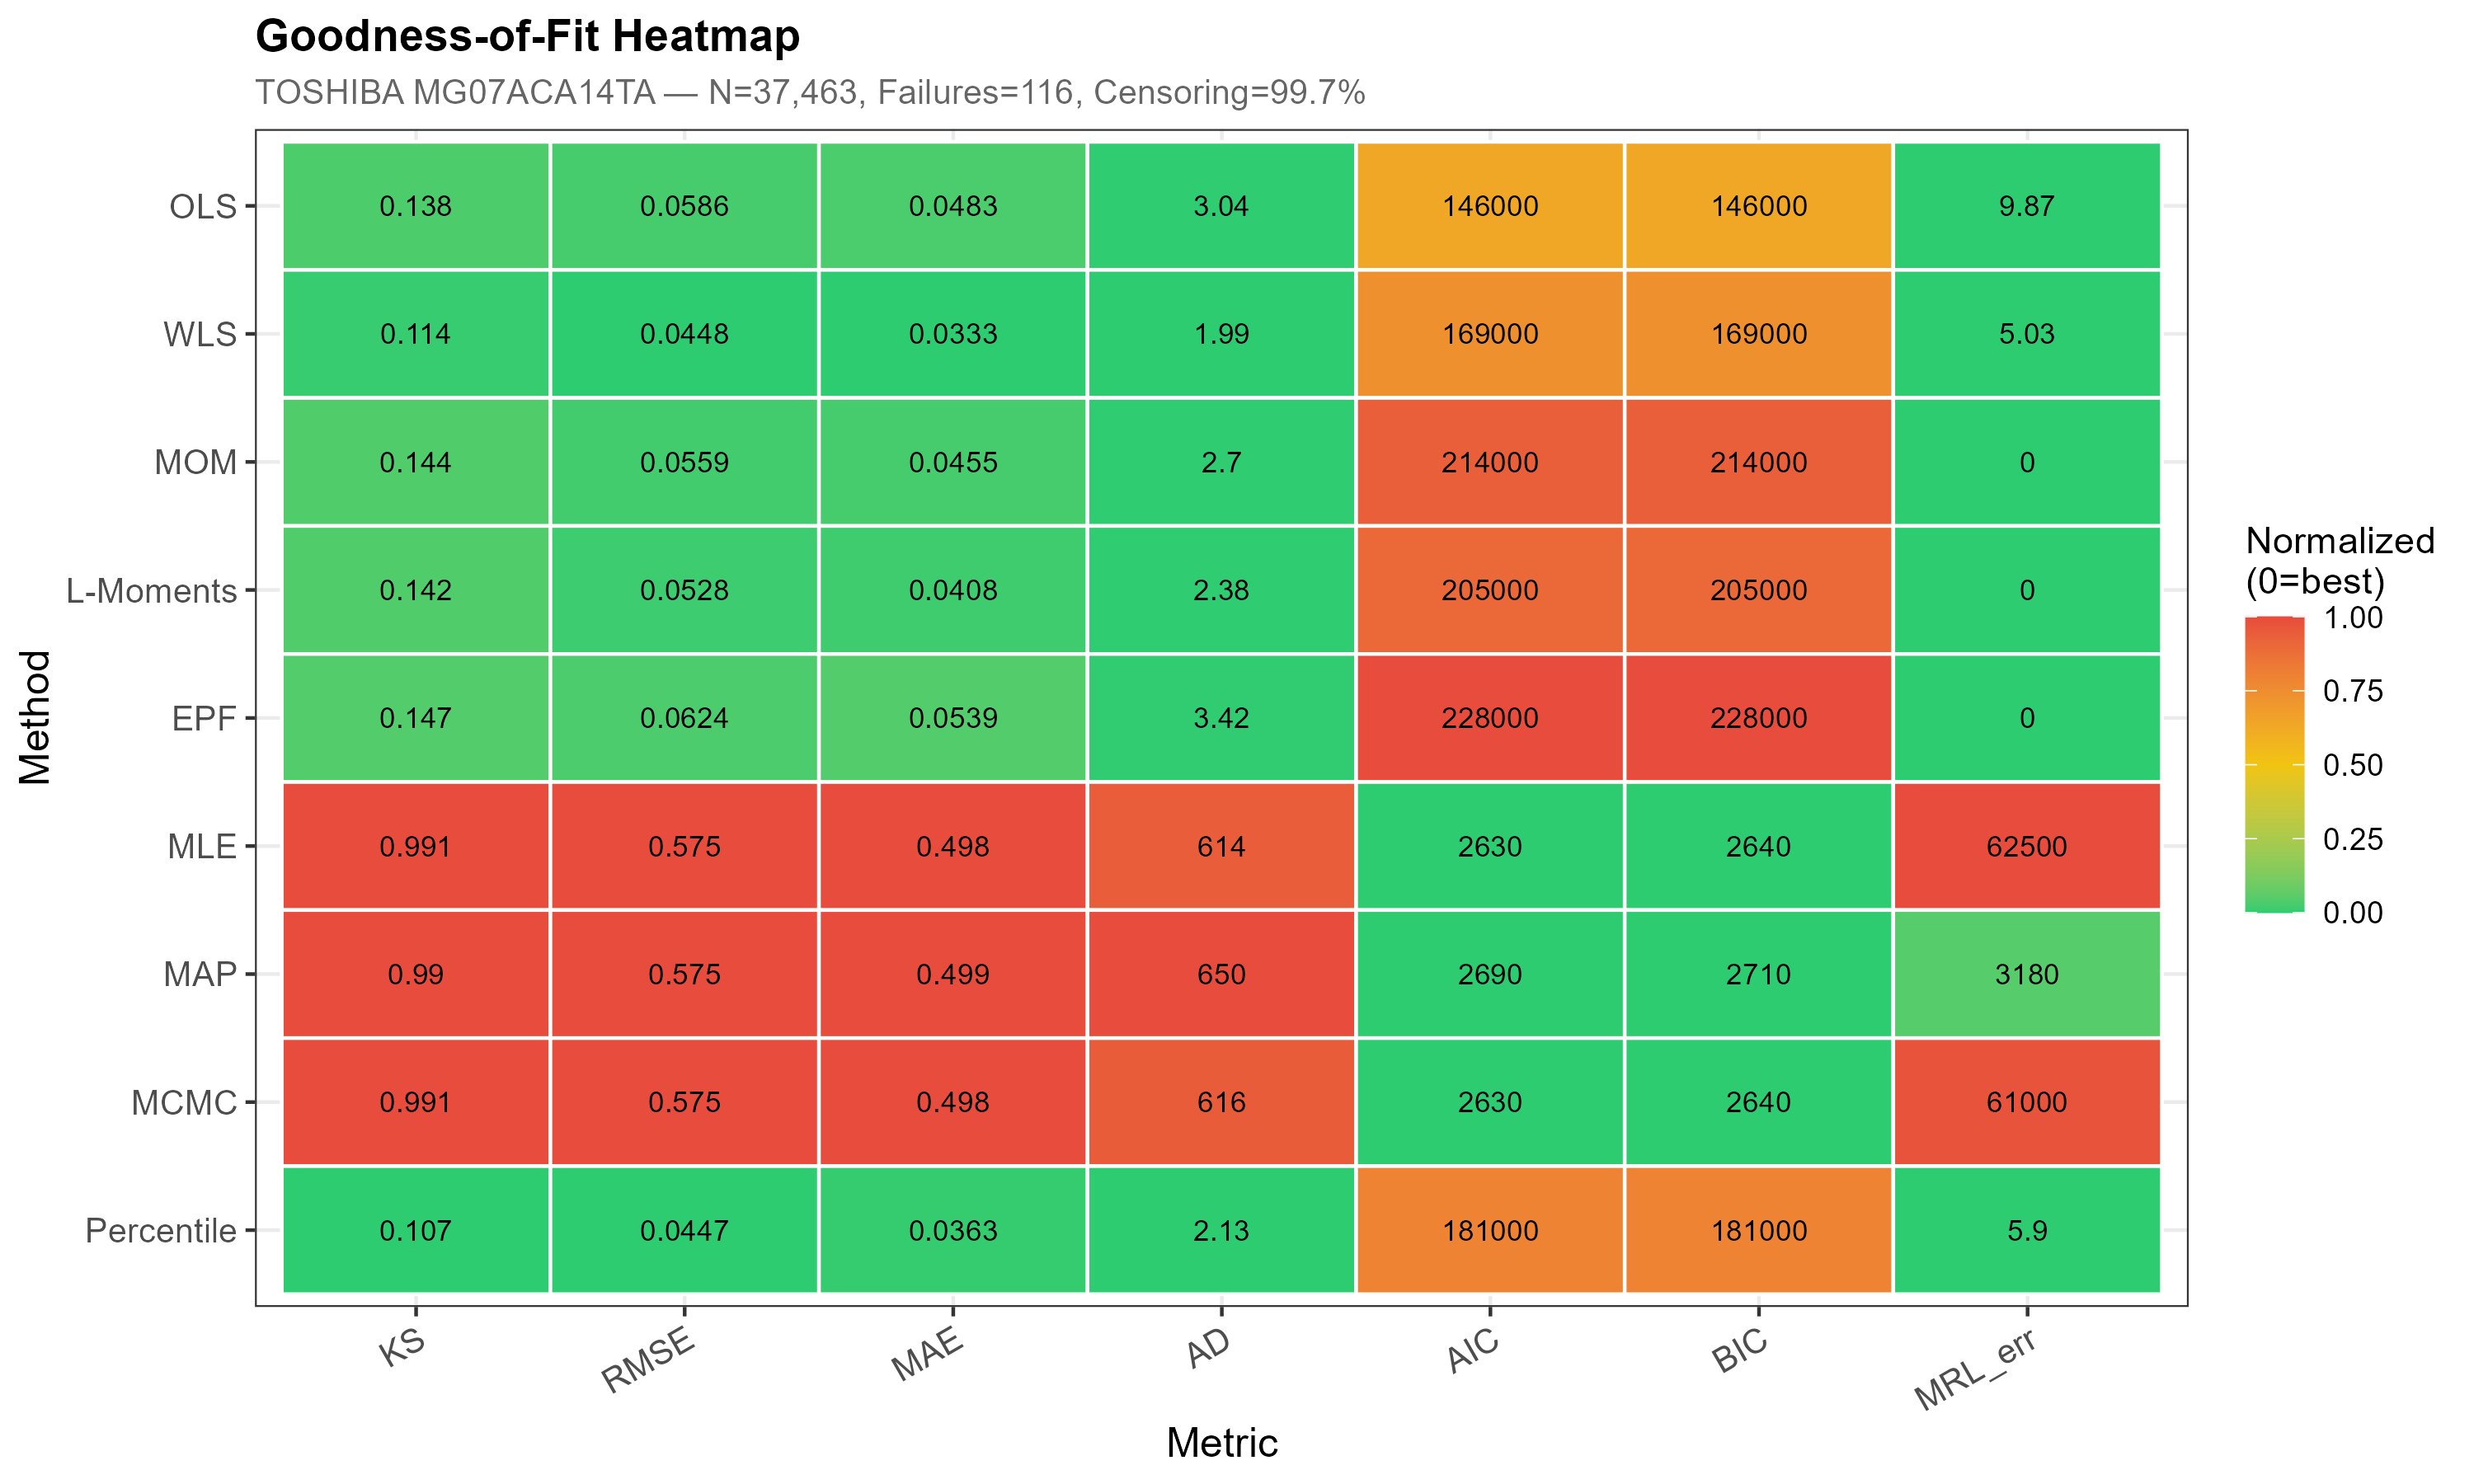
\includegraphics[width=0.95\linewidth]{results/plots/plot6_gof_heatmap_TOSHIBA_MG07ACA14TA.png}
\caption{GoF Heatmap — TOSHIBA MG07ACA14TA}
\end{figure}

\subsubsection{TOSHIBA MG08ACA16TA}\label{toshiba-mg08aca16ta}

\begin{figure}[H]
\centering
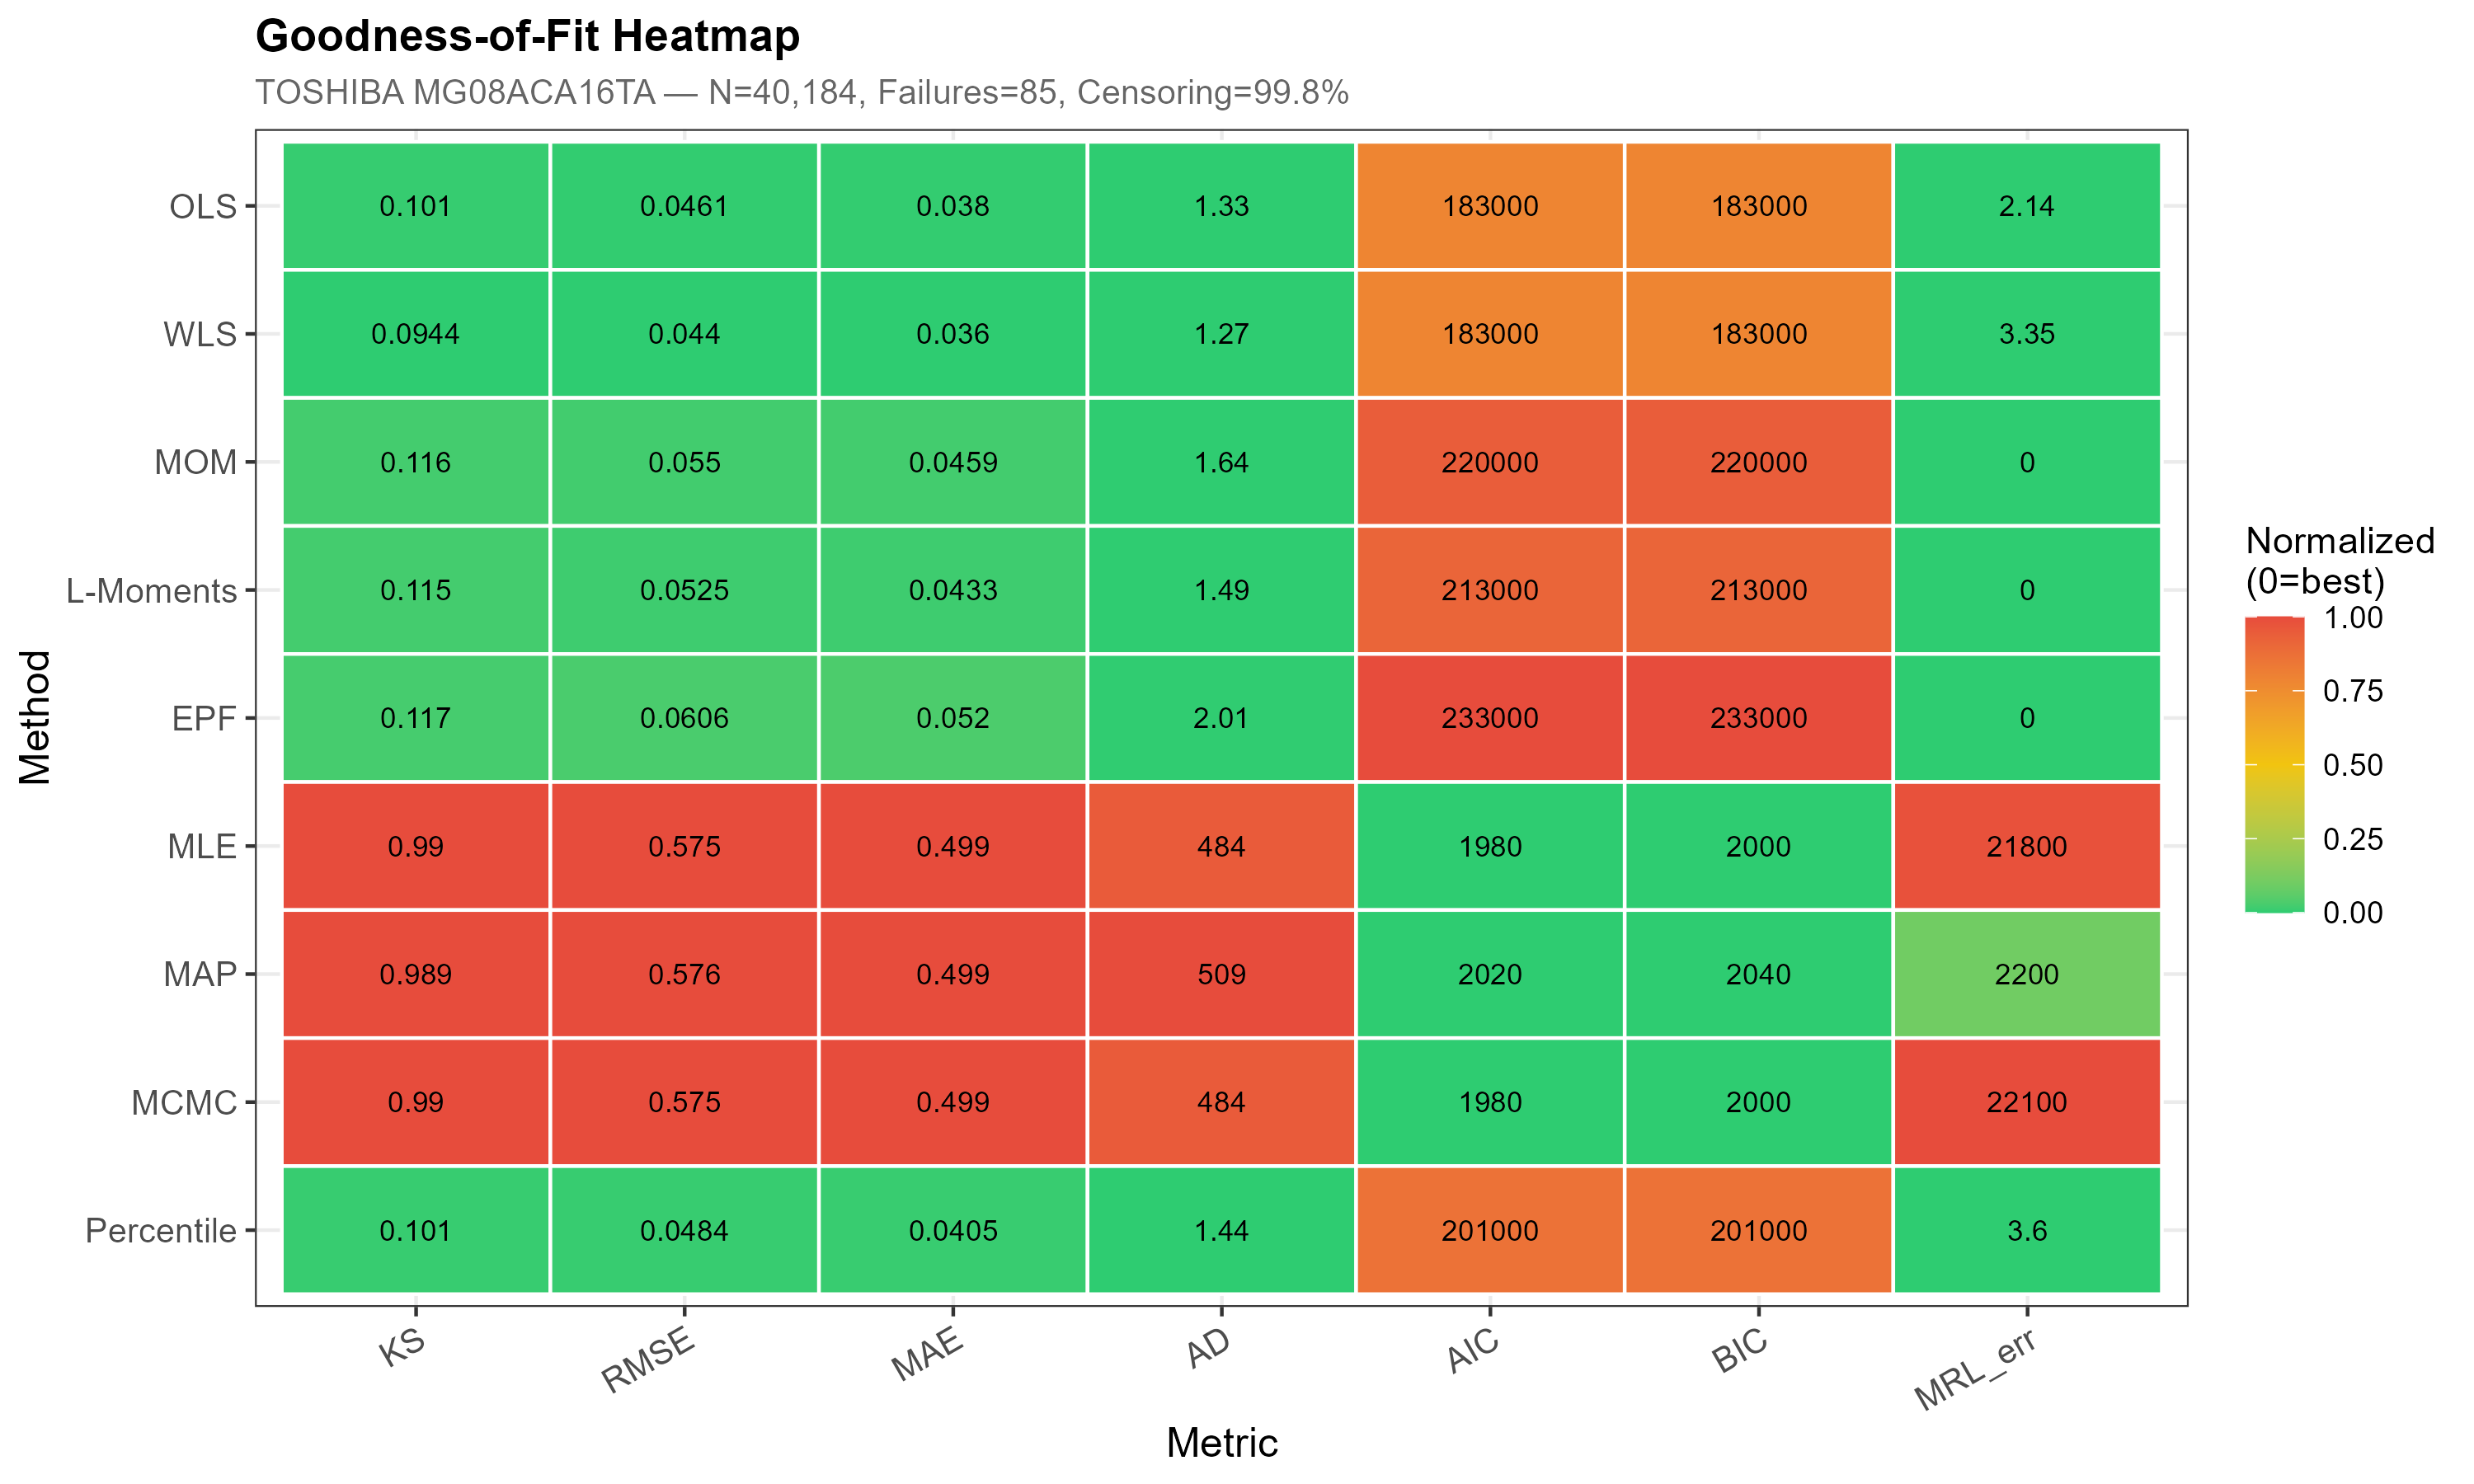
\includegraphics[width=0.95\linewidth]{results/plots/plot6_gof_heatmap_TOSHIBA_MG08ACA16TA.png}
\caption{GoF Heatmap — TOSHIBA MG08ACA16TA}
\end{figure}

\subsubsection{WDC WUH722222ALE6L4}\label{wdc-wuh722222ale6l4}

\begin{figure}[H]
\centering
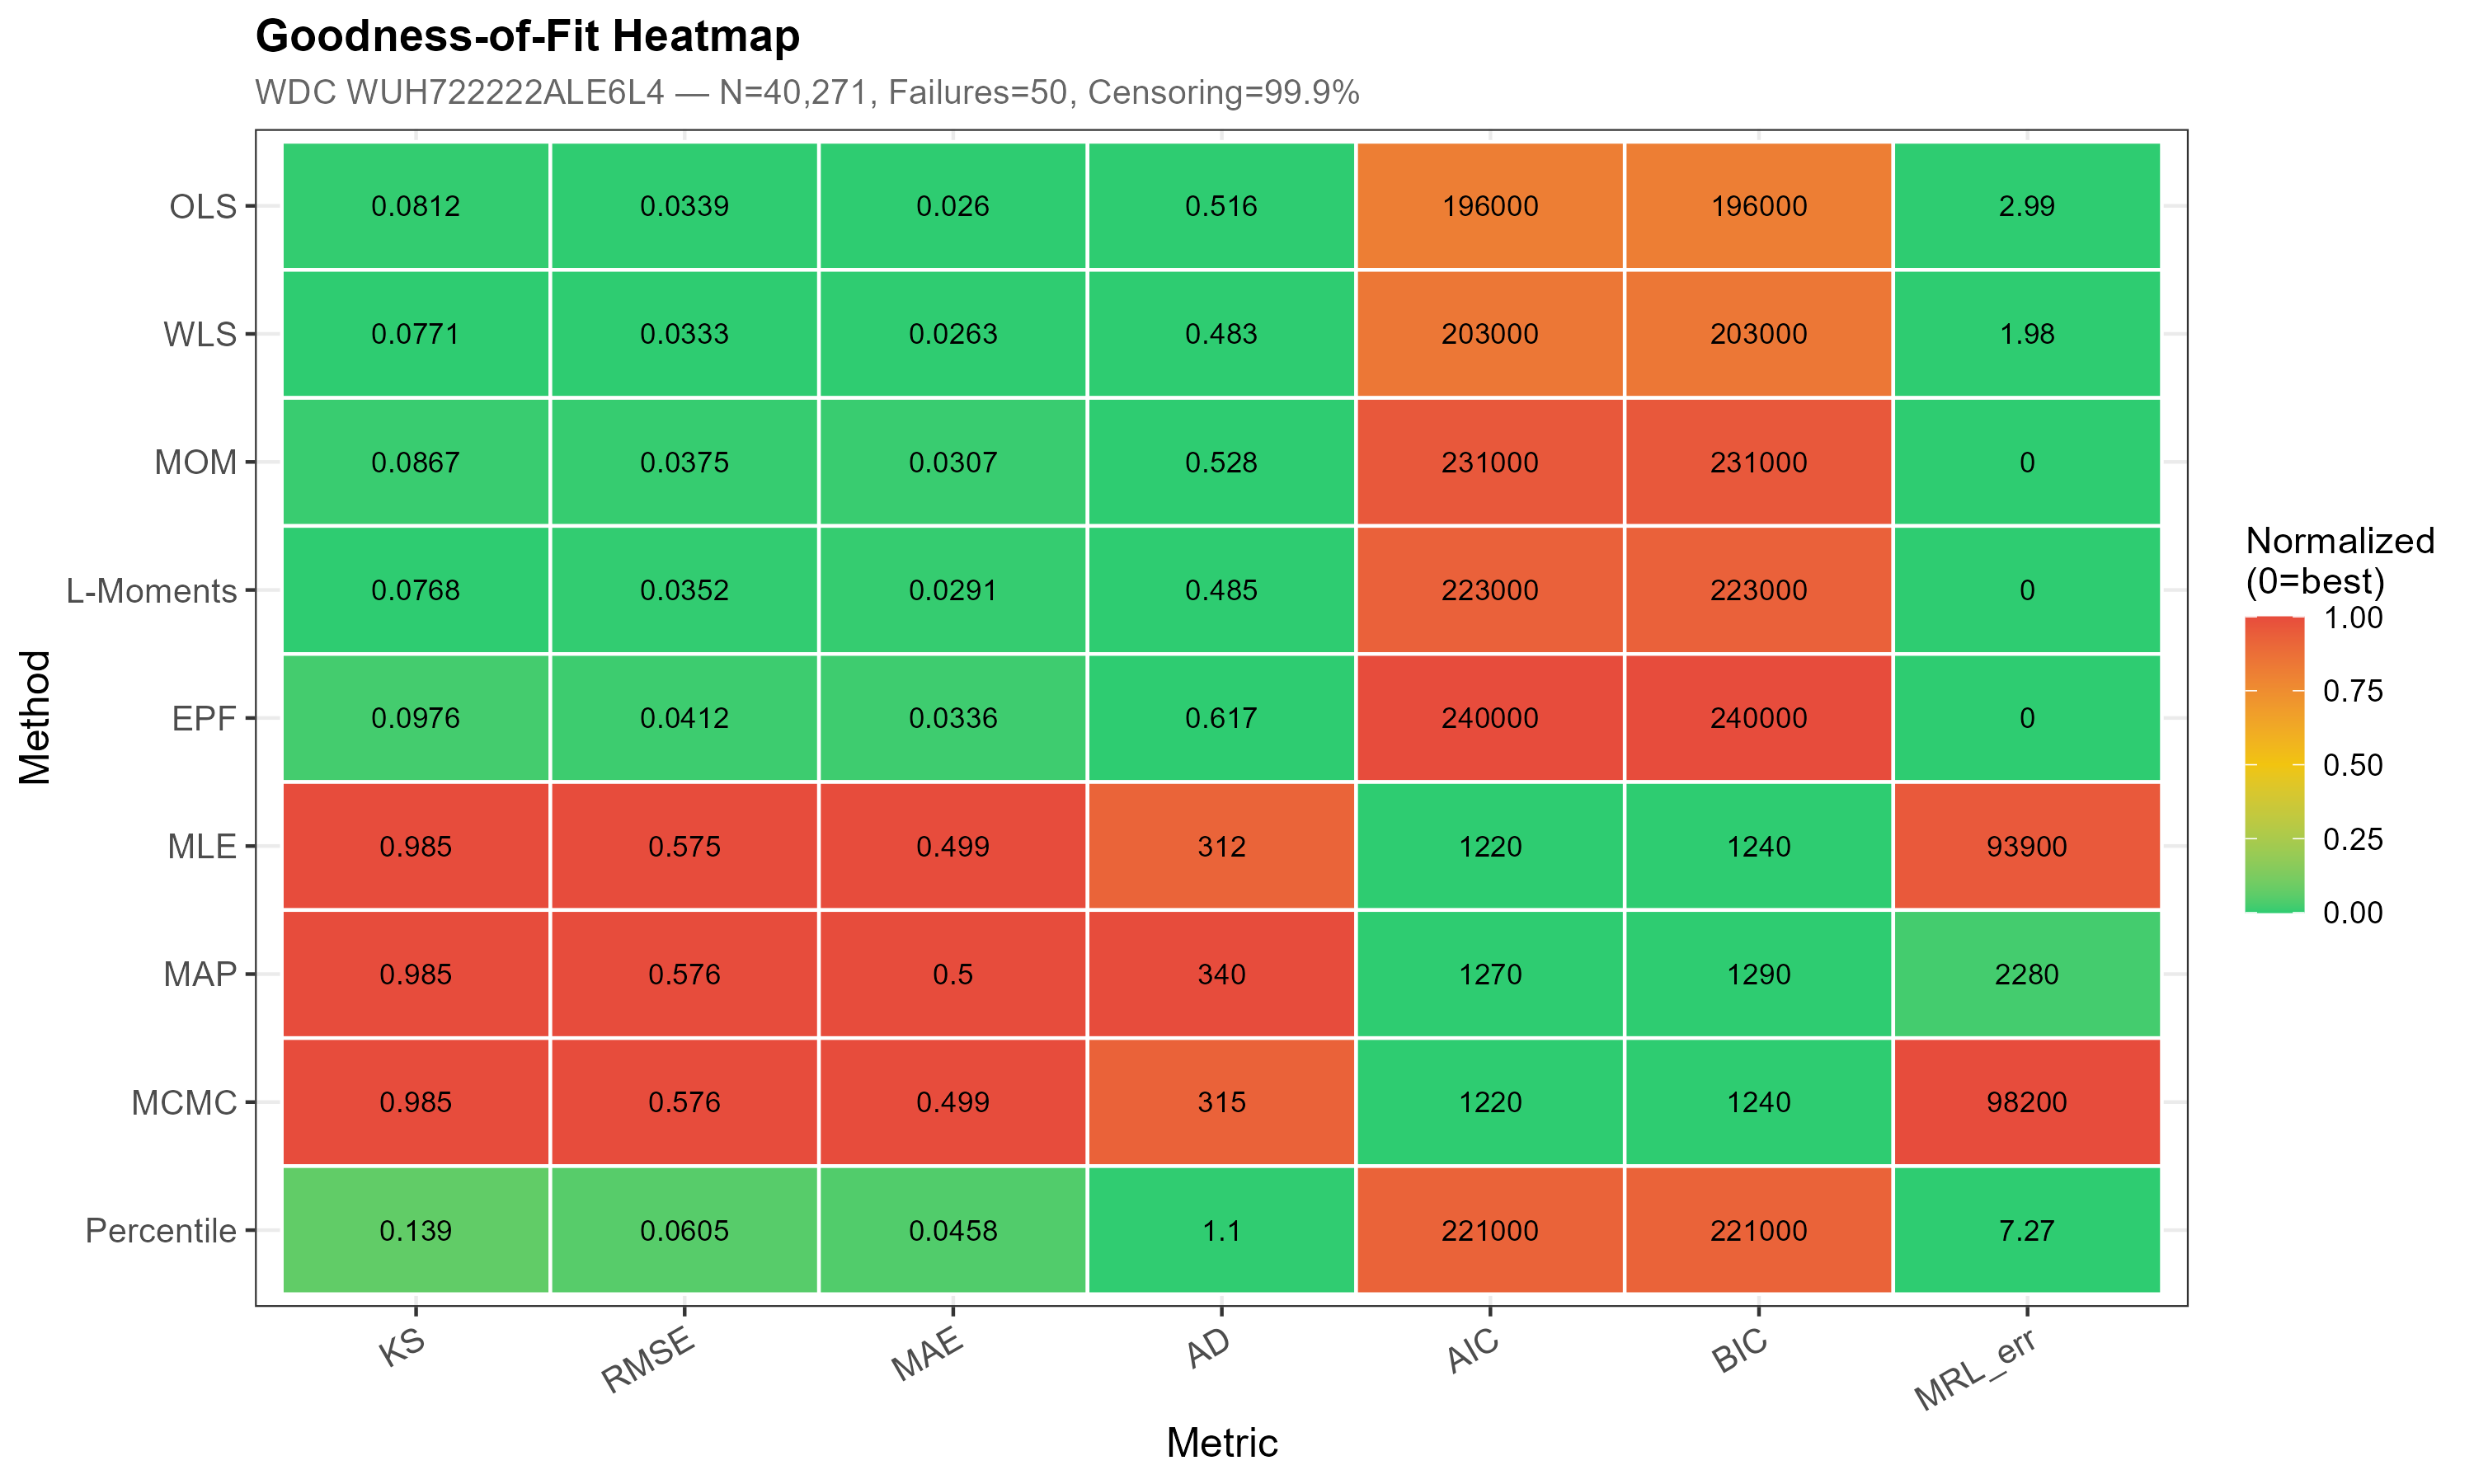
\includegraphics[width=0.95\linewidth]{results/plots/plot6_gof_heatmap_WDC_WUH722222ALE6L4.png}
\caption{GoF Heatmap — WDC WUH722222ALE6L4}
\end{figure}

\begingroup\fontsize{7}{9}\selectfont

\begin{longtable}[t]{llrrrrrrrr}
\caption{\label{tab:table-5-gof}Table 5: Full GoF Metrics}\\
\toprule
model & method & KS & RMSE & MAE & AD & AIC & BIC & MRL\_err & Composite\_Rank\\
\midrule
\endfirsthead
\caption[]{Table 5: Full GoF Metrics \textit{(continued)}}\\
\toprule
model & method & KS & RMSE & MAE & AD & AIC & BIC & MRL\_err & Composite\_Rank\\
\midrule
\endhead

\endfoot
\bottomrule
\endlastfoot
\cellcolor{gray!10}{TOSHIBA MG07ACA14TA} & \cellcolor{gray!10}{OLS} & \cellcolor{gray!10}{0.1375} & \cellcolor{gray!10}{0.0586} & \cellcolor{gray!10}{0.0483} & \cellcolor{gray!10}{3.0372} & \cellcolor{gray!10}{146091.89} & \cellcolor{gray!10}{146108.96} & \cellcolor{gray!10}{9.8674} & \cellcolor{gray!10}{4.6667}\\
TOSHIBA MG07ACA14TA & WLS & 0.1145 & 0.0448 & 0.0333 & 1.9922 & 169173.38 & 169190.44 & 5.0273 & 2.6667\\
\cellcolor{gray!10}{TOSHIBA MG07ACA14TA} & \cellcolor{gray!10}{MOM} & \cellcolor{gray!10}{0.1438} & \cellcolor{gray!10}{0.0559} & \cellcolor{gray!10}{0.0455} & \cellcolor{gray!10}{2.7008} & \cellcolor{gray!10}{213664.93} & \cellcolor{gray!10}{213681.99} & \cellcolor{gray!10}{0.0000} & \cellcolor{gray!10}{5.3333}\\
TOSHIBA MG07ACA14TA & L-Moments & 0.1424 & 0.0528 & 0.0408 & 2.3834 & 204906.10 & 204923.16 & 0.0000 & 4.3333\\
\cellcolor{gray!10}{TOSHIBA MG07ACA14TA} & \cellcolor{gray!10}{EPF} & \cellcolor{gray!10}{0.1465} & \cellcolor{gray!10}{0.0624} & \cellcolor{gray!10}{0.0539} & \cellcolor{gray!10}{3.4181} & \cellcolor{gray!10}{228190.01} & \cellcolor{gray!10}{228207.07} & \cellcolor{gray!10}{0.0000} & \cellcolor{gray!10}{7.0000}\\
\addlinespace
TOSHIBA MG07ACA14TA & MLE & 0.9909 & 0.5751 & 0.4985 & 613.5523 & 2625.06 & 2642.12 & 62475.2337 & 5.0000\\
\cellcolor{gray!10}{TOSHIBA MG07ACA14TA} & \cellcolor{gray!10}{MAP} & \cellcolor{gray!10}{0.9904} & \cellcolor{gray!10}{0.5753} & \cellcolor{gray!10}{0.4988} & \cellcolor{gray!10}{650.2219} & \cellcolor{gray!10}{2690.00} & \cellcolor{gray!10}{2707.07} & \cellcolor{gray!10}{3180.7688} & \cellcolor{gray!10}{7.0000}\\
TOSHIBA MG07ACA14TA & MCMC & 0.9910 & 0.5751 & 0.4985 & 616.2851 & 2625.11 & 2642.18 & 61025.6853 & 6.0000\\
\cellcolor{gray!10}{TOSHIBA MG07ACA14TA} & \cellcolor{gray!10}{Percentile} & \cellcolor{gray!10}{0.1069} & \cellcolor{gray!10}{0.0447} & \cellcolor{gray!10}{0.0363} & \cellcolor{gray!10}{2.1256} & \cellcolor{gray!10}{181286.55} & \cellcolor{gray!10}{181303.61} & \cellcolor{gray!10}{5.8995} & \cellcolor{gray!10}{3.0000}\\
TOSHIBA MG08ACA16TA & OLS & 0.1011 & 0.0461 & 0.0380 & 1.3347 & 183367.08 & 183384.28 & 2.1435 & 3.0000\\
\addlinespace
\cellcolor{gray!10}{TOSHIBA MG08ACA16TA} & \cellcolor{gray!10}{WLS} & \cellcolor{gray!10}{0.0944} & \cellcolor{gray!10}{0.0440} & \cellcolor{gray!10}{0.0360} & \cellcolor{gray!10}{1.2738} & \cellcolor{gray!10}{183248.73} & \cellcolor{gray!10}{183265.93} & \cellcolor{gray!10}{3.3479} & \cellcolor{gray!10}{2.0000}\\
TOSHIBA MG08ACA16TA & MOM & 0.1155 & 0.0550 & 0.0459 & 1.6371 & 220231.31 & 220248.51 & 0.0000 & 6.0000\\
\cellcolor{gray!10}{TOSHIBA MG08ACA16TA} & \cellcolor{gray!10}{L-Moments} & \cellcolor{gray!10}{0.1148} & \cellcolor{gray!10}{0.0525} & \cellcolor{gray!10}{0.0433} & \cellcolor{gray!10}{1.4942} & \cellcolor{gray!10}{213201.08} & \cellcolor{gray!10}{213218.28} & \cellcolor{gray!10}{0.0000} & \cellcolor{gray!10}{5.0000}\\
TOSHIBA MG08ACA16TA & EPF & 0.1171 & 0.0606 & 0.0520 & 2.0052 & 233235.08 & 233252.28 & 0.0000 & 7.0000\\
\cellcolor{gray!10}{TOSHIBA MG08ACA16TA} & \cellcolor{gray!10}{MLE} & \cellcolor{gray!10}{0.9897} & \cellcolor{gray!10}{0.5755} & \cellcolor{gray!10}{0.4990} & \cellcolor{gray!10}{483.6366} & \cellcolor{gray!10}{1984.96} & \cellcolor{gray!10}{2002.16} & \cellcolor{gray!10}{21779.7631} & \cellcolor{gray!10}{5.0000}\\
\addlinespace
TOSHIBA MG08ACA16TA & MAP & 0.9894 & 0.5756 & 0.4992 & 508.9463 & 2022.05 & 2039.25 & 2198.1787 & 7.0000\\
\cellcolor{gray!10}{TOSHIBA MG08ACA16TA} & \cellcolor{gray!10}{MCMC} & \cellcolor{gray!10}{0.9897} & \cellcolor{gray!10}{0.5755} & \cellcolor{gray!10}{0.4990} & \cellcolor{gray!10}{483.9352} & \cellcolor{gray!10}{1984.96} & \cellcolor{gray!10}{2002.16} & \cellcolor{gray!10}{22134.5002} & \cellcolor{gray!10}{6.0000}\\
TOSHIBA MG08ACA16TA & Percentile & 0.1015 & 0.0484 & 0.0405 & 1.4440 & 201296.62 & 201313.82 & 3.5974 & 4.0000\\
\cellcolor{gray!10}{WDC WUH722222ALE6L4} & \cellcolor{gray!10}{OLS} & \cellcolor{gray!10}{0.0812} & \cellcolor{gray!10}{0.0339} & \cellcolor{gray!10}{0.0260} & \cellcolor{gray!10}{0.5157} & \cellcolor{gray!10}{195793.10} & \cellcolor{gray!10}{195810.31} & \cellcolor{gray!10}{2.9896} & \cellcolor{gray!10}{3.0000}\\
WDC WUH722222ALE6L4 & WLS & 0.0771 & 0.0333 & 0.0263 & 0.4831 & 202583.28 & 202600.48 & 1.9775 & 2.3333\\
\addlinespace
\cellcolor{gray!10}{WDC WUH722222ALE6L4} & \cellcolor{gray!10}{MOM} & \cellcolor{gray!10}{0.0867} & \cellcolor{gray!10}{0.0375} & \cellcolor{gray!10}{0.0307} & \cellcolor{gray!10}{0.5275} & \cellcolor{gray!10}{230700.18} & \cellcolor{gray!10}{230717.39} & \cellcolor{gray!10}{0.0000} & \cellcolor{gray!10}{5.3333}\\
WDC WUH722222ALE6L4 & L-Moments & 0.0768 & 0.0352 & 0.0291 & 0.4846 & 223111.68 & 223128.89 & 0.0000 & 4.0000\\
\cellcolor{gray!10}{WDC WUH722222ALE6L4} & \cellcolor{gray!10}{EPF} & \cellcolor{gray!10}{0.0976} & \cellcolor{gray!10}{0.0412} & \cellcolor{gray!10}{0.0336} & \cellcolor{gray!10}{0.6171} & \cellcolor{gray!10}{239868.14} & \cellcolor{gray!10}{239885.34} & \cellcolor{gray!10}{0.0000} & \cellcolor{gray!10}{6.3333}\\
WDC WUH722222ALE6L4 & MLE & 0.9848 & 0.5755 & 0.4994 & 312.0262 & 1220.91 & 1238.12 & 93911.4541 & 5.0000\\
\cellcolor{gray!10}{WDC WUH722222ALE6L4} & \cellcolor{gray!10}{MAP} & \cellcolor{gray!10}{0.9845} & \cellcolor{gray!10}{0.5756} & \cellcolor{gray!10}{0.4996} & \cellcolor{gray!10}{340.4928} & \cellcolor{gray!10}{1271.91} & \cellcolor{gray!10}{1289.12} & \cellcolor{gray!10}{2276.5954} & \cellcolor{gray!10}{7.0000}\\
\addlinespace
WDC WUH722222ALE6L4 & MCMC & 0.9849 & 0.5755 & 0.4994 & 315.2097 & 1221.10 & 1238.31 & 98178.1975 & 6.0000\\
\cellcolor{gray!10}{WDC WUH722222ALE6L4} & \cellcolor{gray!10}{Percentile} & \cellcolor{gray!10}{0.1392} & \cellcolor{gray!10}{0.0605} & \cellcolor{gray!10}{0.0458} & \cellcolor{gray!10}{1.0983} & \cellcolor{gray!10}{220752.17} & \cellcolor{gray!10}{220769.37} & \cellcolor{gray!10}{7.2683} & \cellcolor{gray!10}{6.0000}\\*
\end{longtable}
\endgroup{}

\subsection{Visual Assessment}\label{visual-assessment}

\subsubsection{TOSHIBA MG07ACA14TA}\label{toshiba-mg07aca14ta-1}

\begin{figure}[H]
\centering
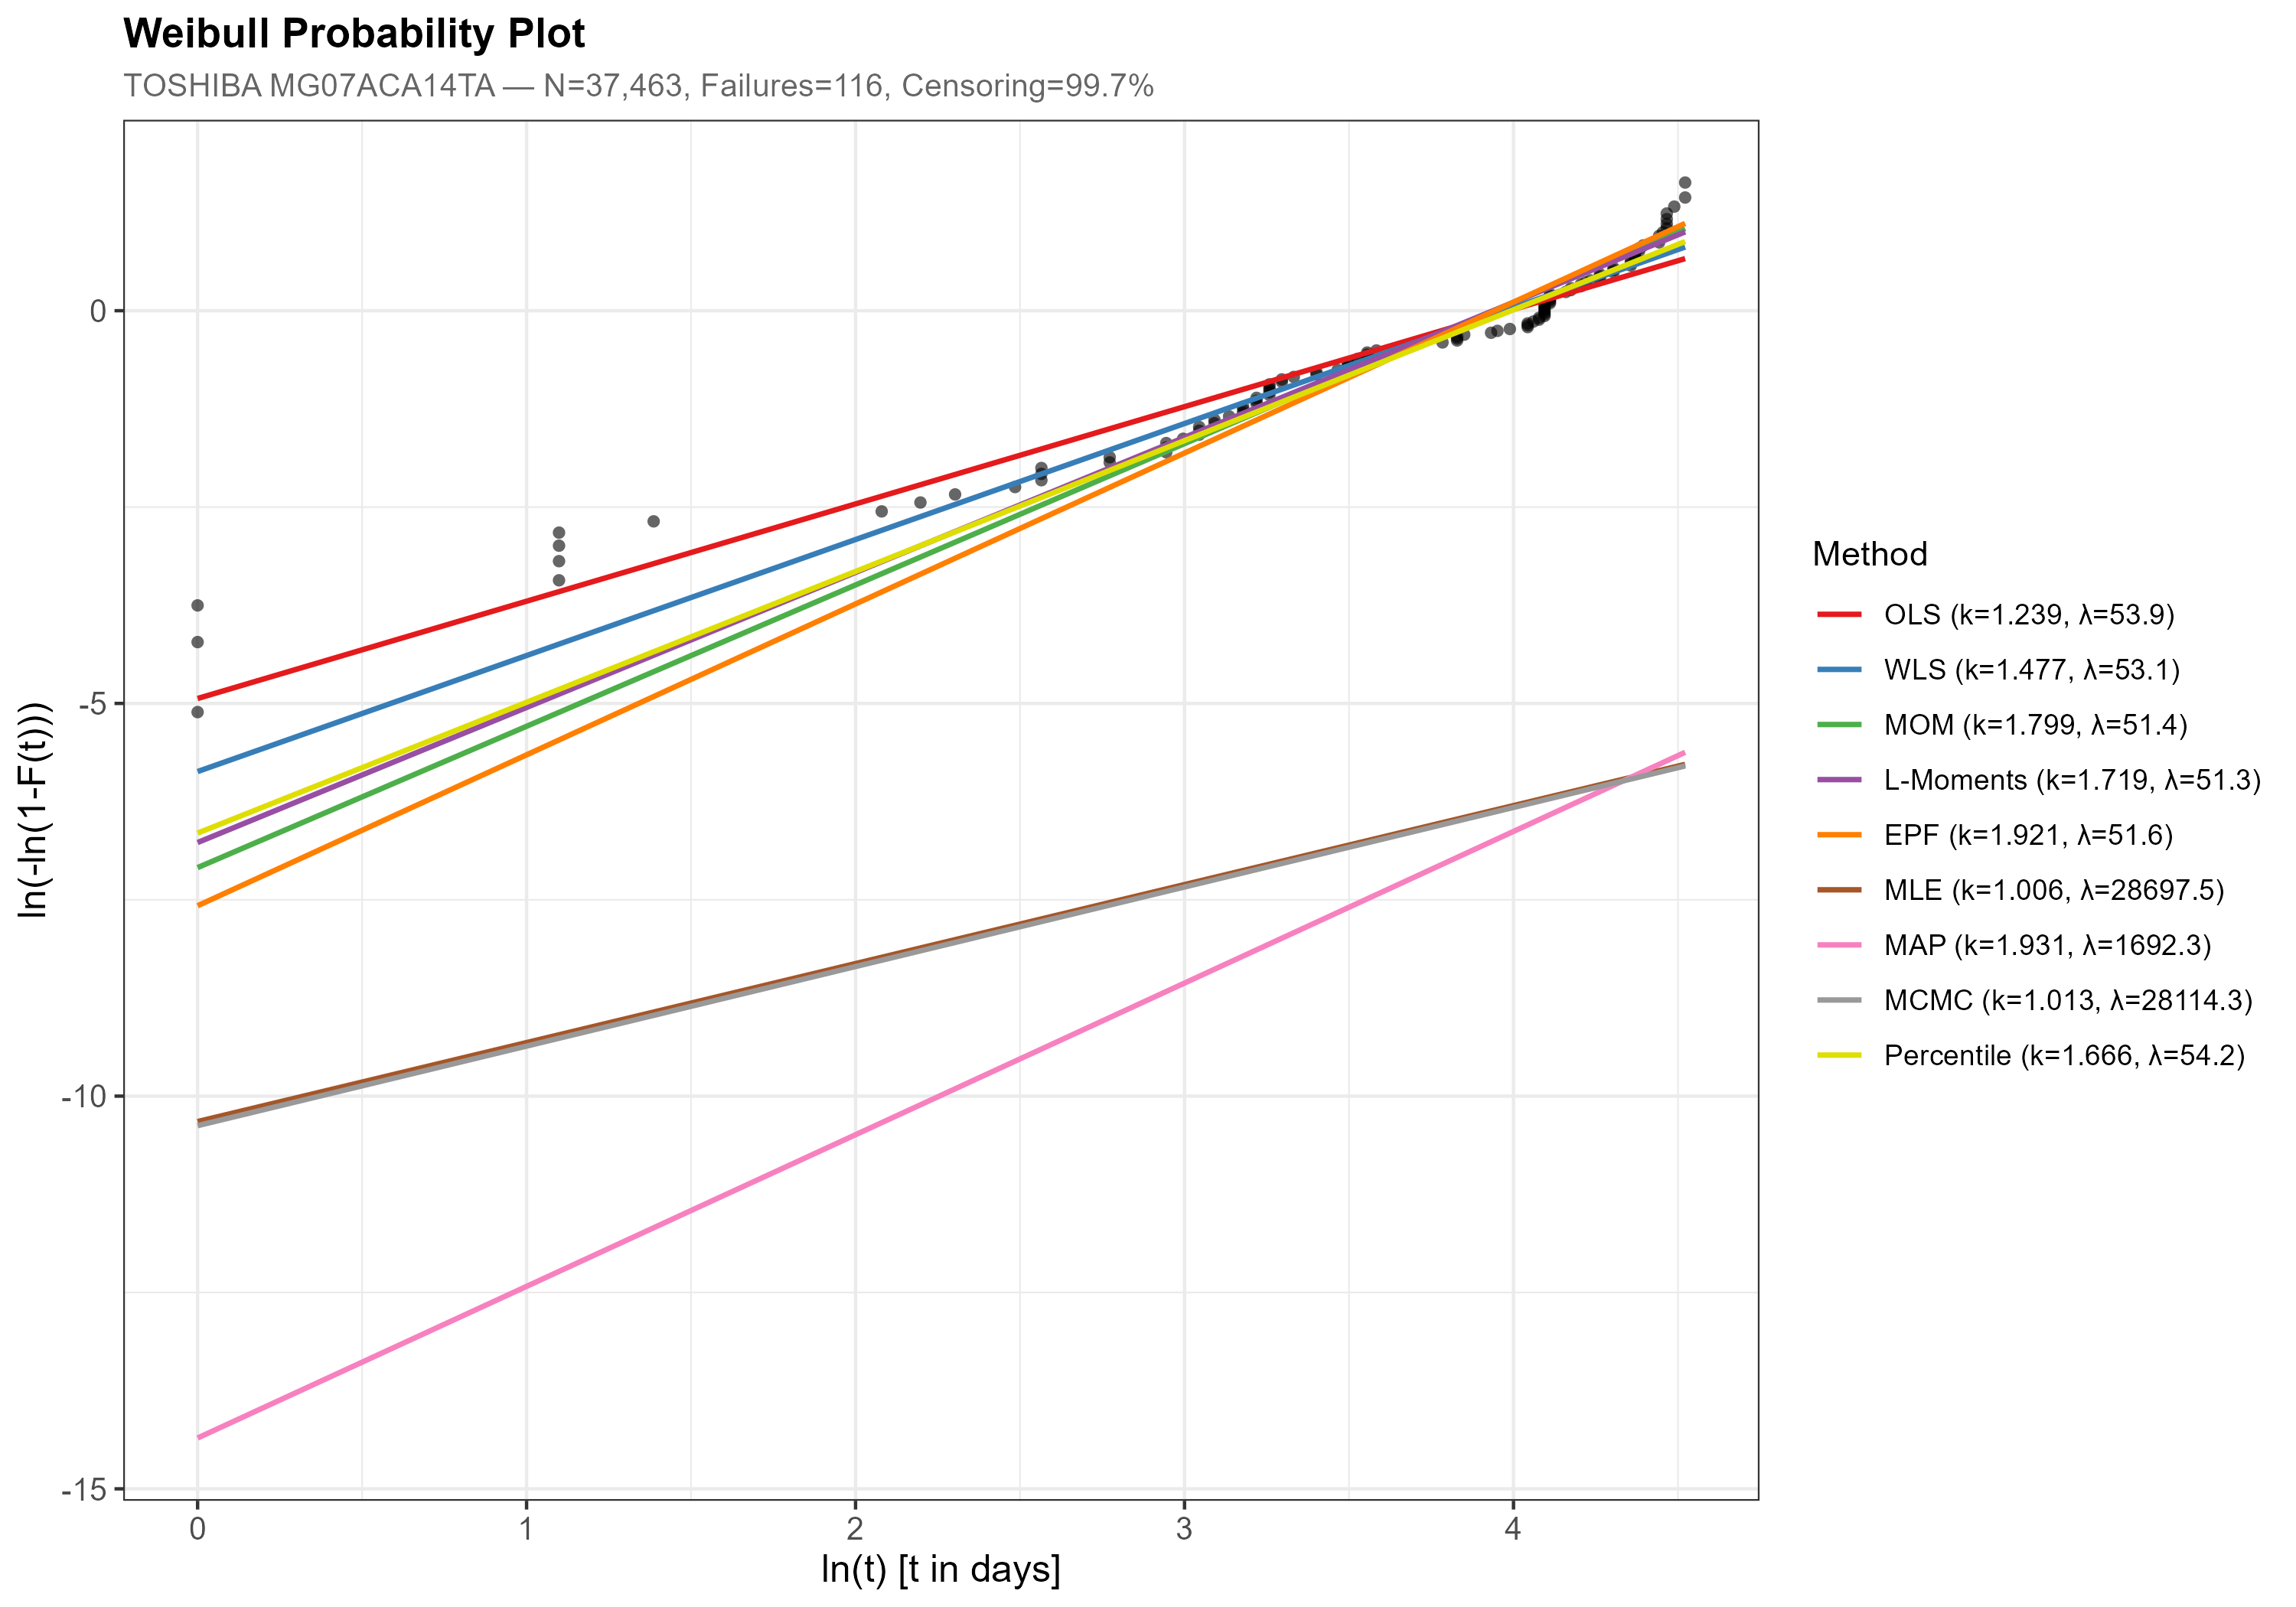
\includegraphics[width=0.9\linewidth]{results/plots/plot1_weibull_probability_TOSHIBA_MG07ACA14TA.png}
\caption{Weibull Probability Plot — TOSHIBA MG07ACA14TA}
\end{figure}

\begin{figure}[H]
\centering
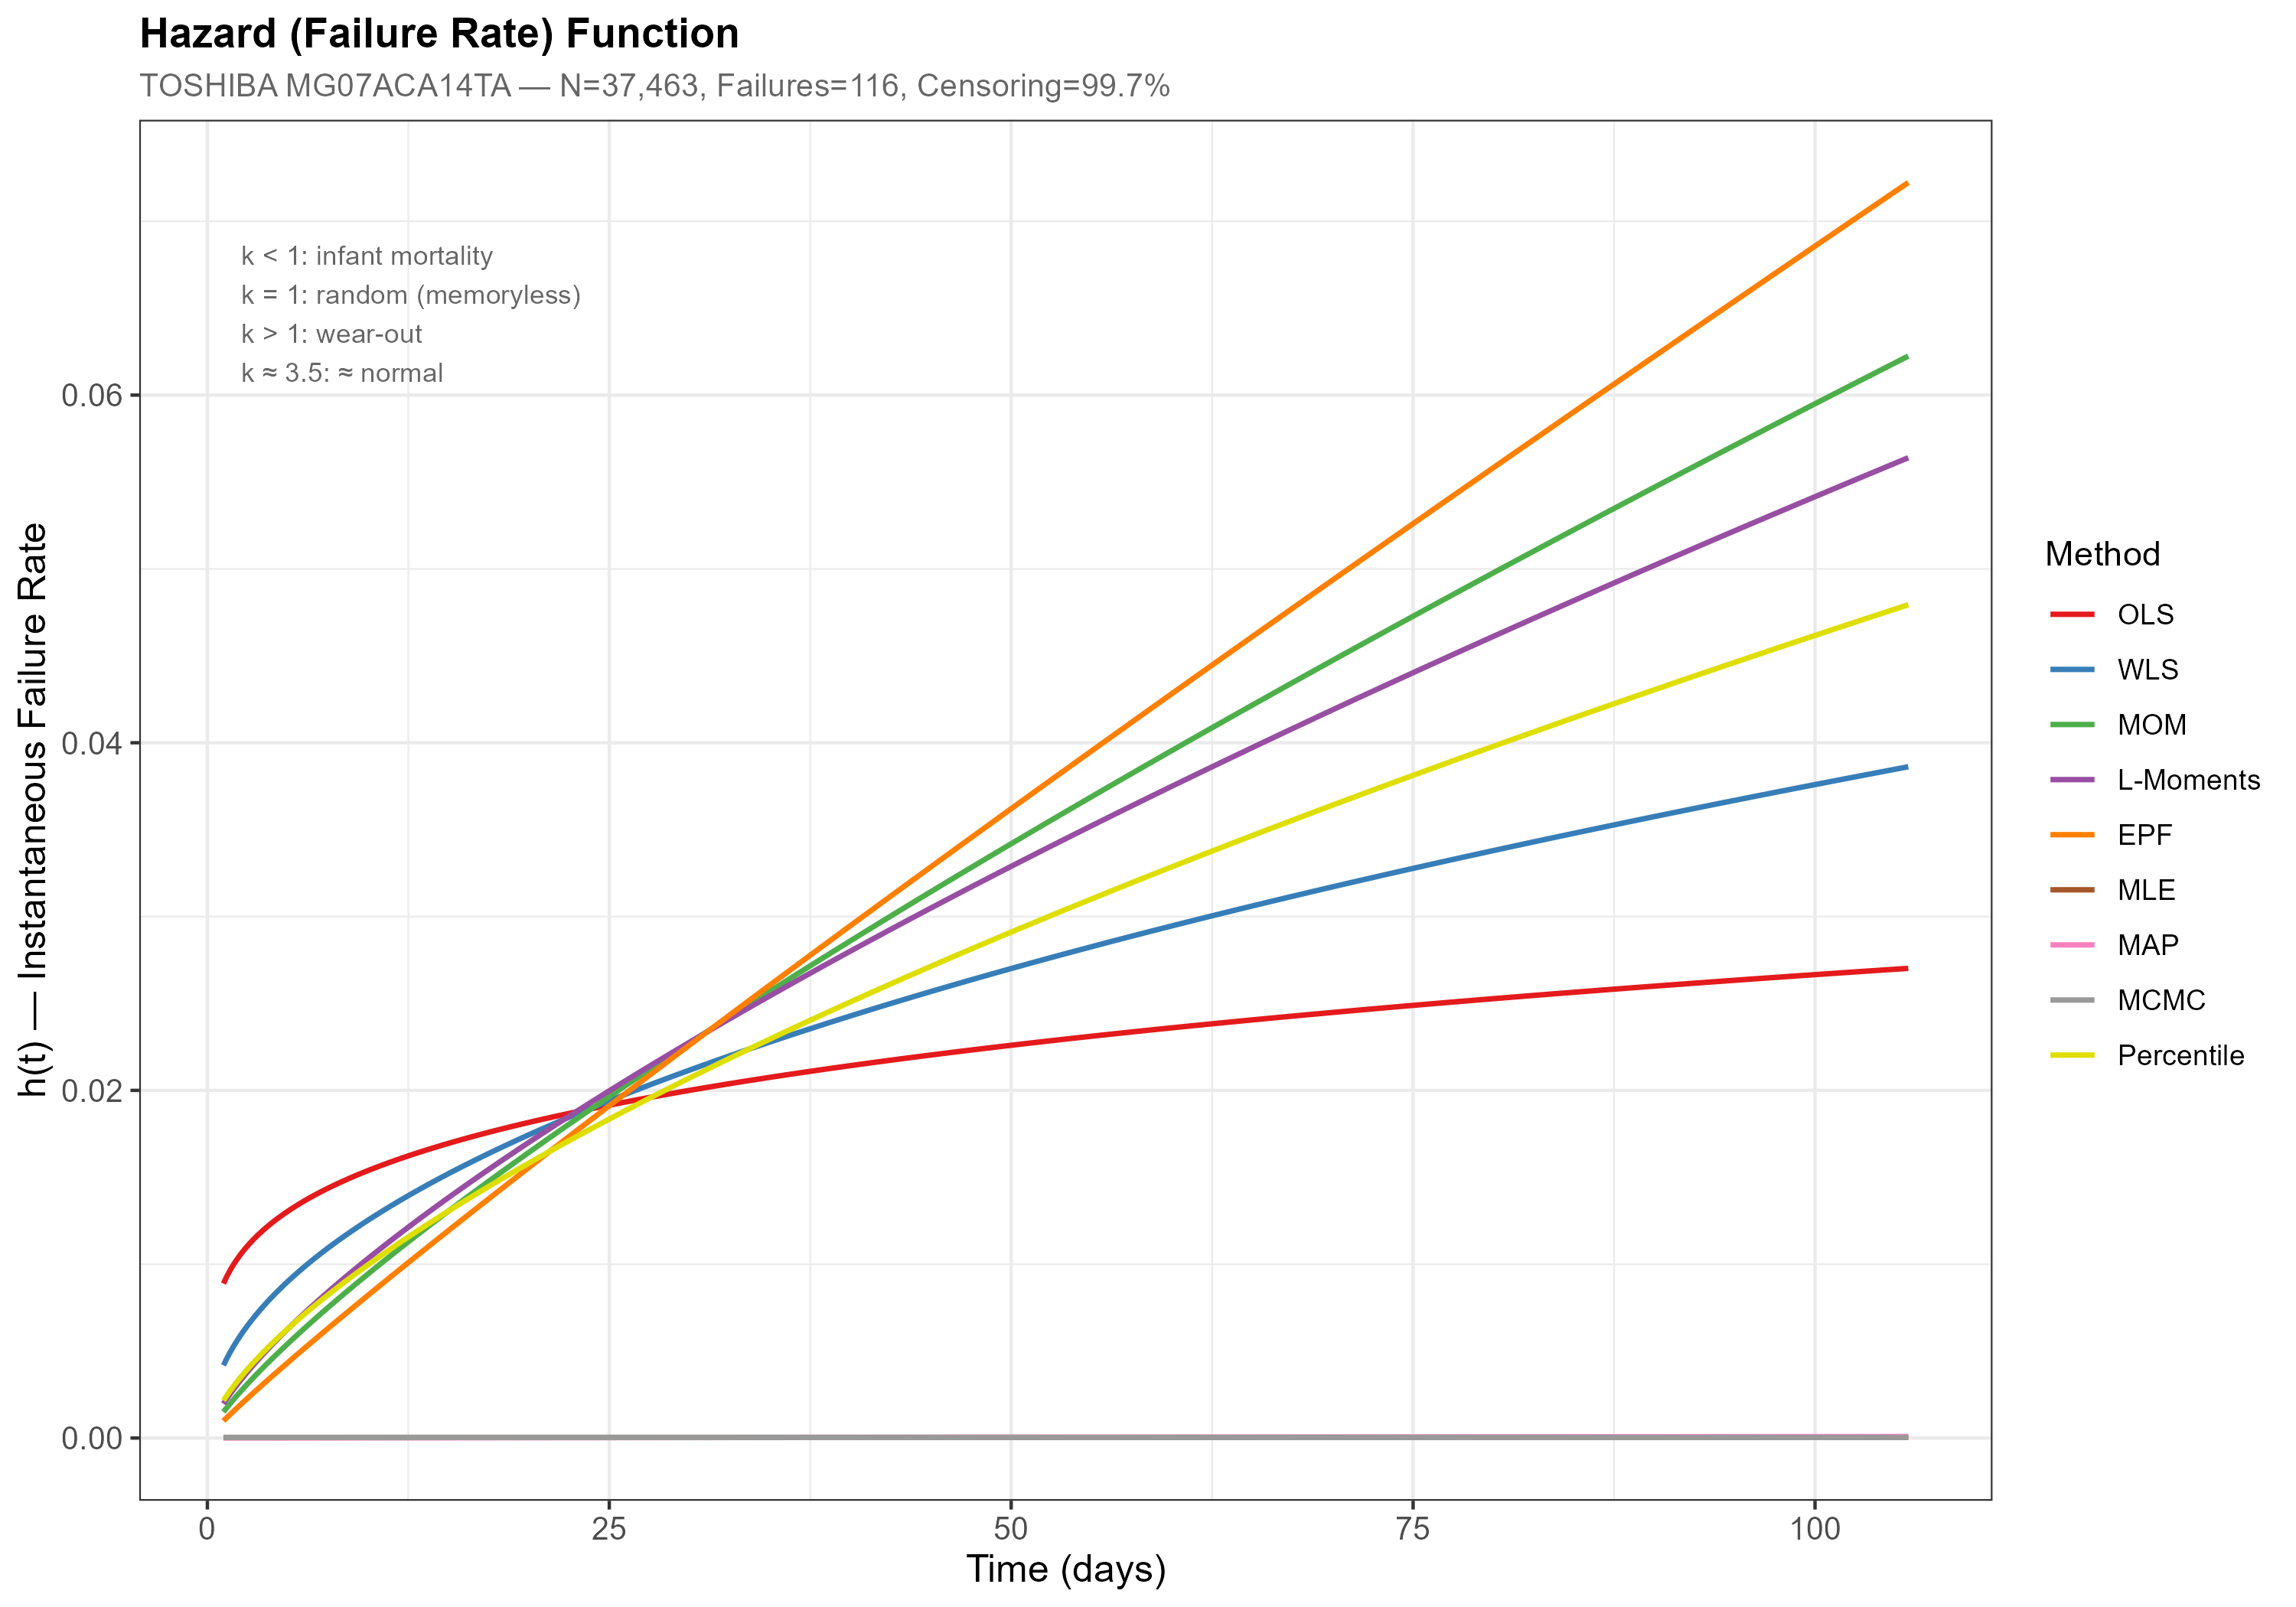
\includegraphics[width=0.9\linewidth]{results/plots/plot5_hazard_TOSHIBA_MG07ACA14TA.png}
\caption{Hazard Function — TOSHIBA MG07ACA14TA}
\end{figure}

\subsubsection{TOSHIBA MG08ACA16TA}\label{toshiba-mg08aca16ta-1}

\begin{figure}[H]
\centering
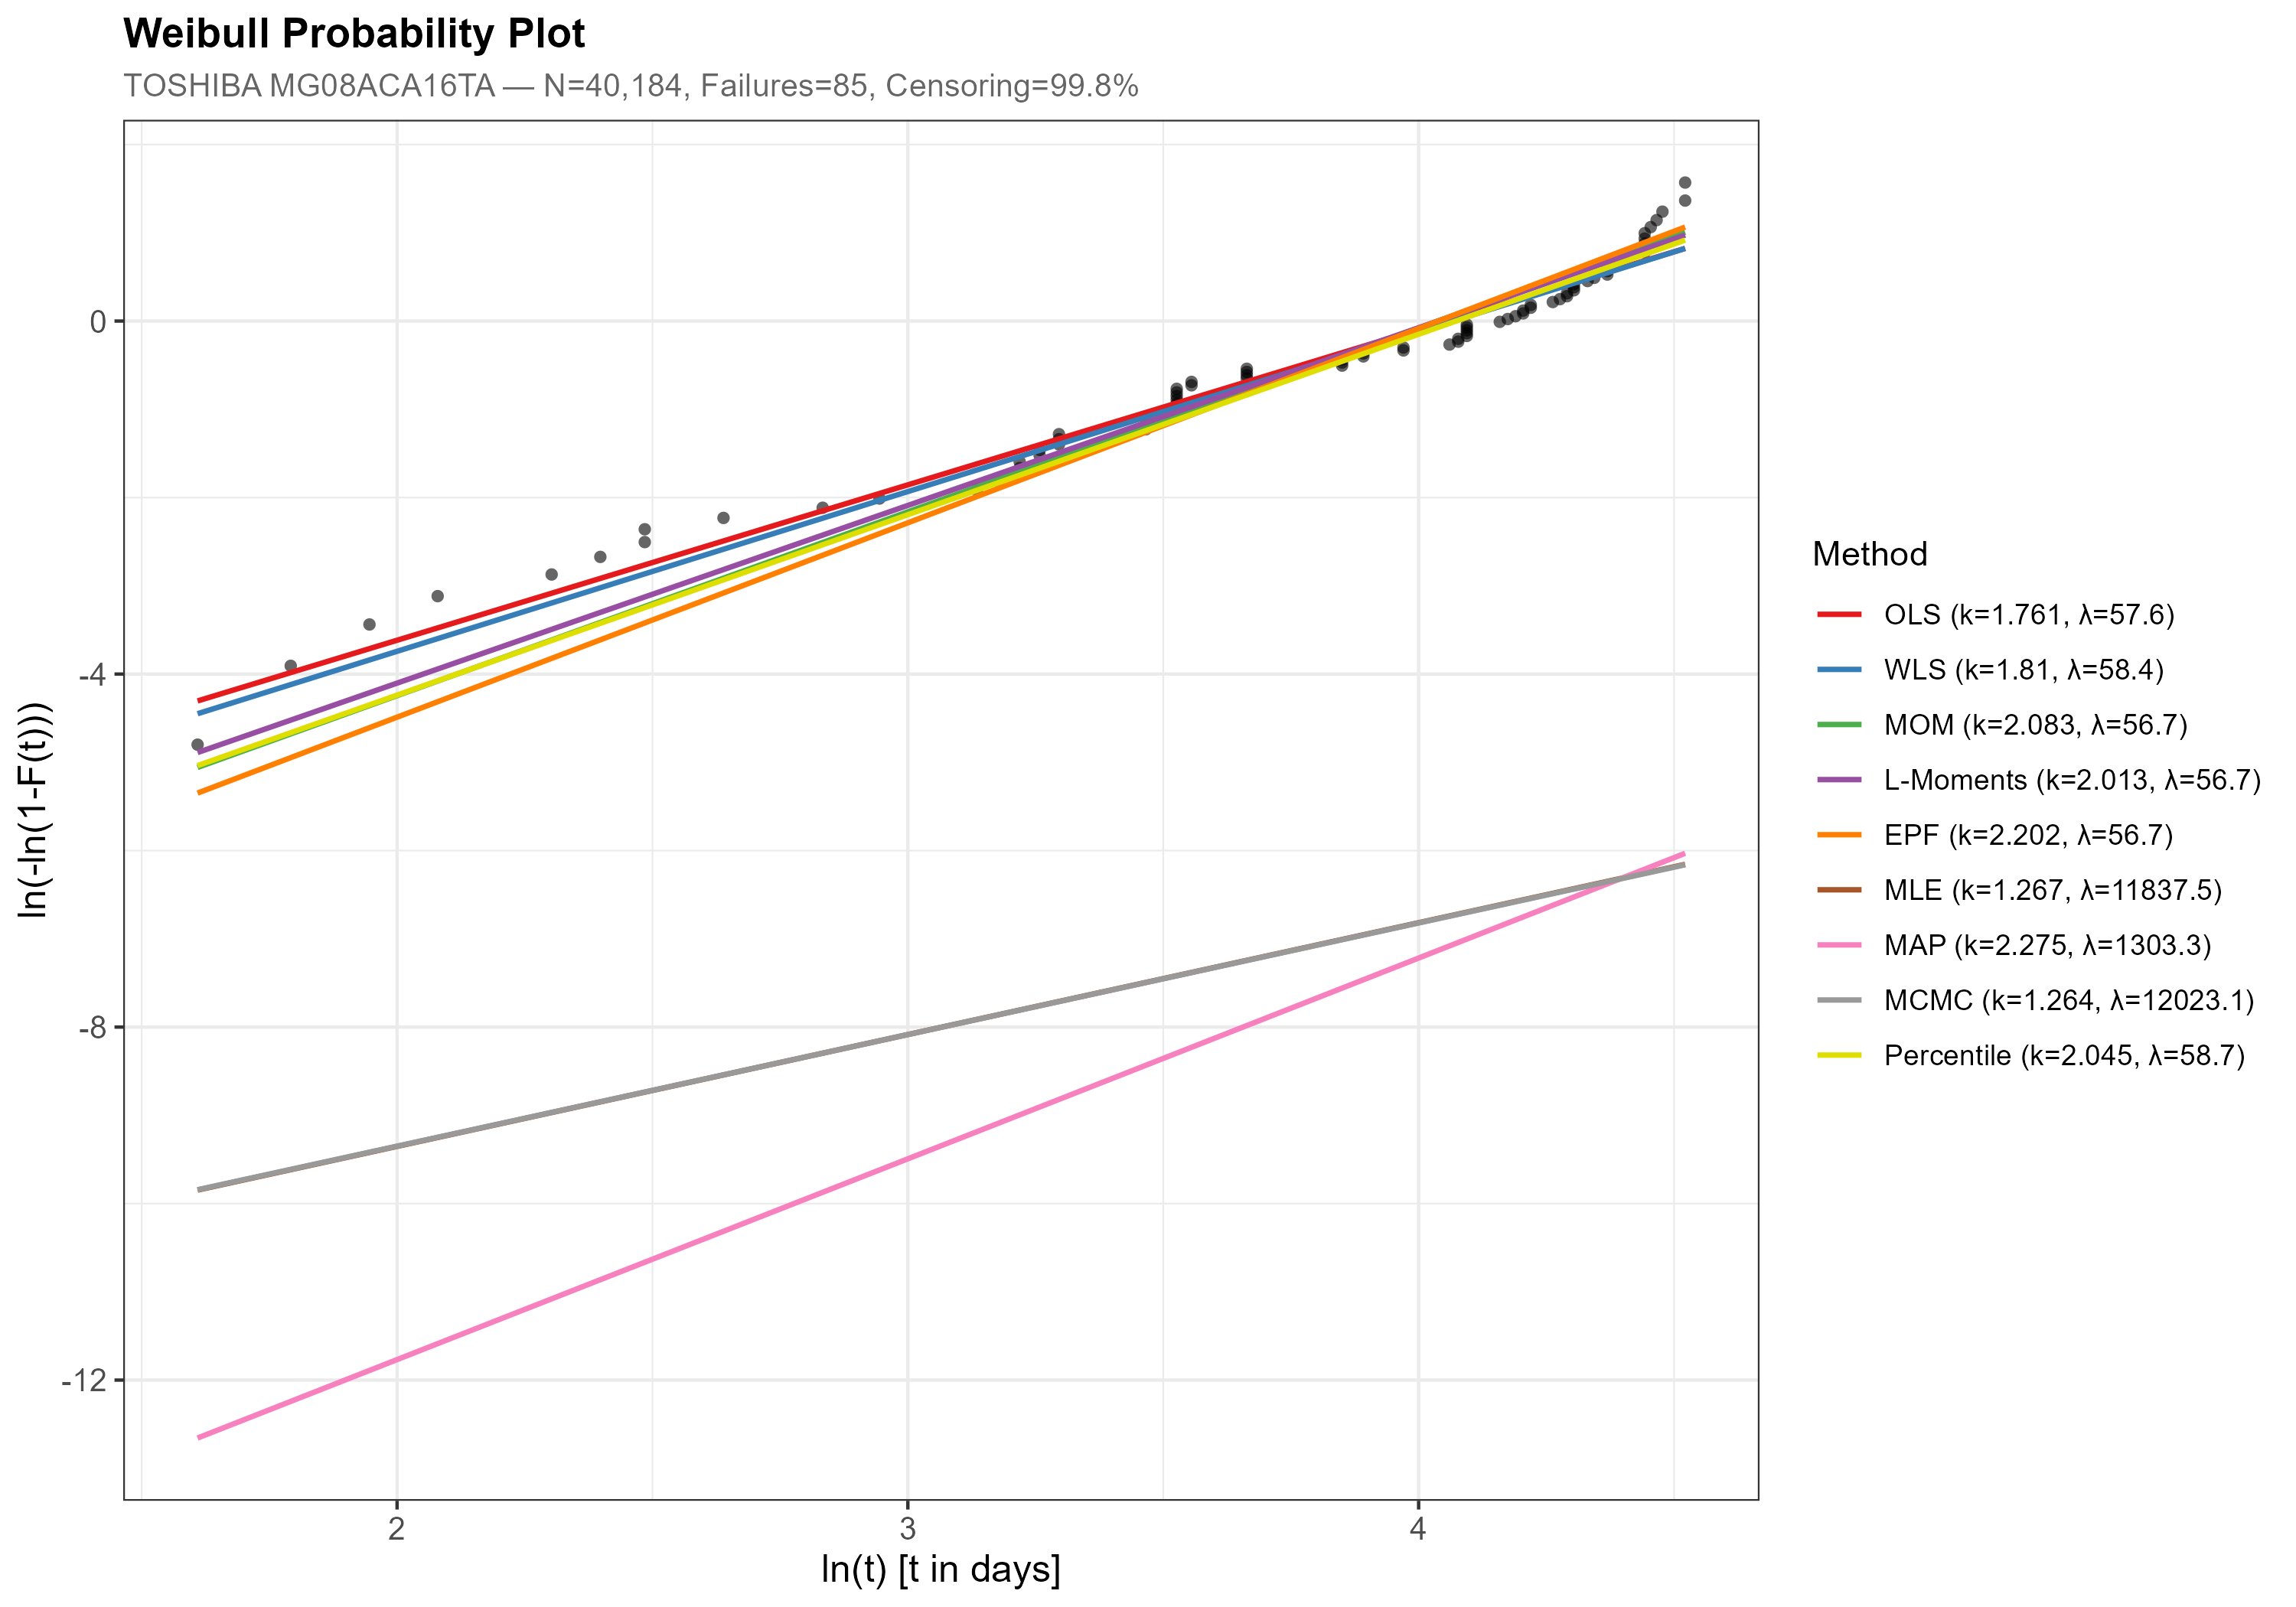
\includegraphics[width=0.9\linewidth]{results/plots/plot1_weibull_probability_TOSHIBA_MG08ACA16TA.png}
\caption{Weibull Probability Plot — TOSHIBA MG08ACA16TA}
\end{figure}

\begin{figure}[H]
\centering
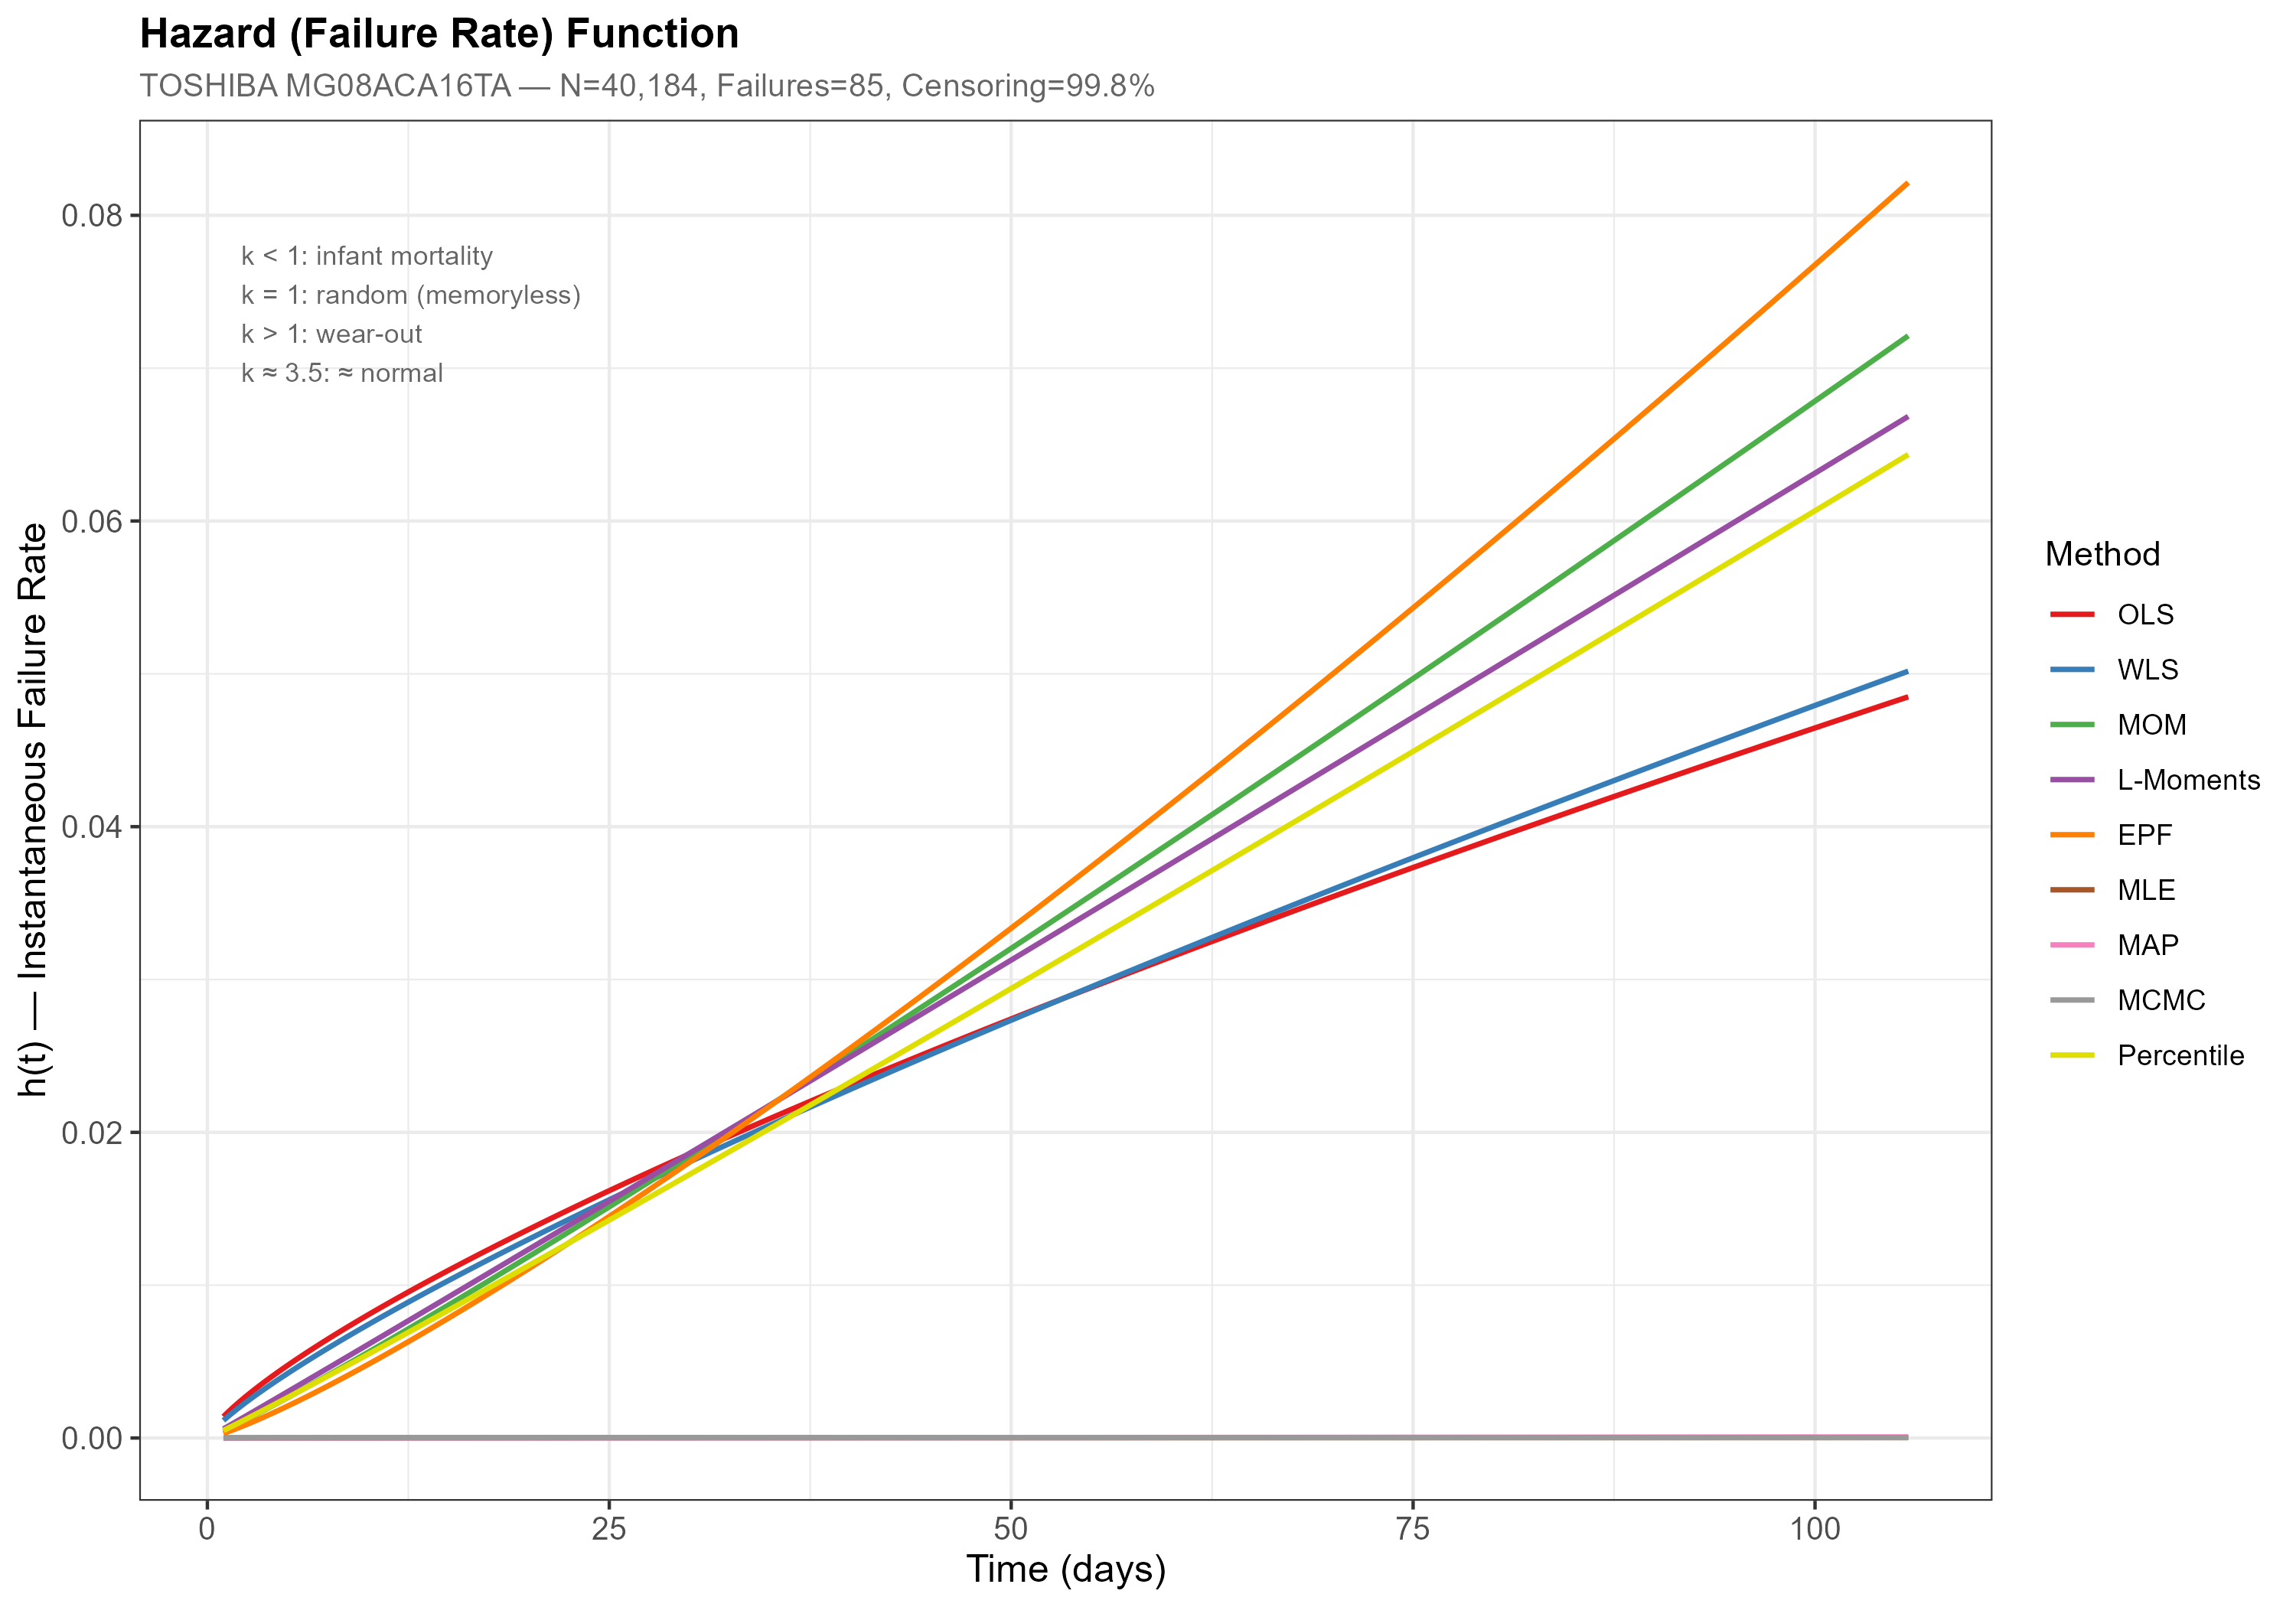
\includegraphics[width=0.9\linewidth]{results/plots/plot5_hazard_TOSHIBA_MG08ACA16TA.png}
\caption{Hazard Function — TOSHIBA MG08ACA16TA}
\end{figure}

\subsubsection{WDC WUH722222ALE6L4}\label{wdc-wuh722222ale6l4-1}

\begin{figure}[H]
\centering
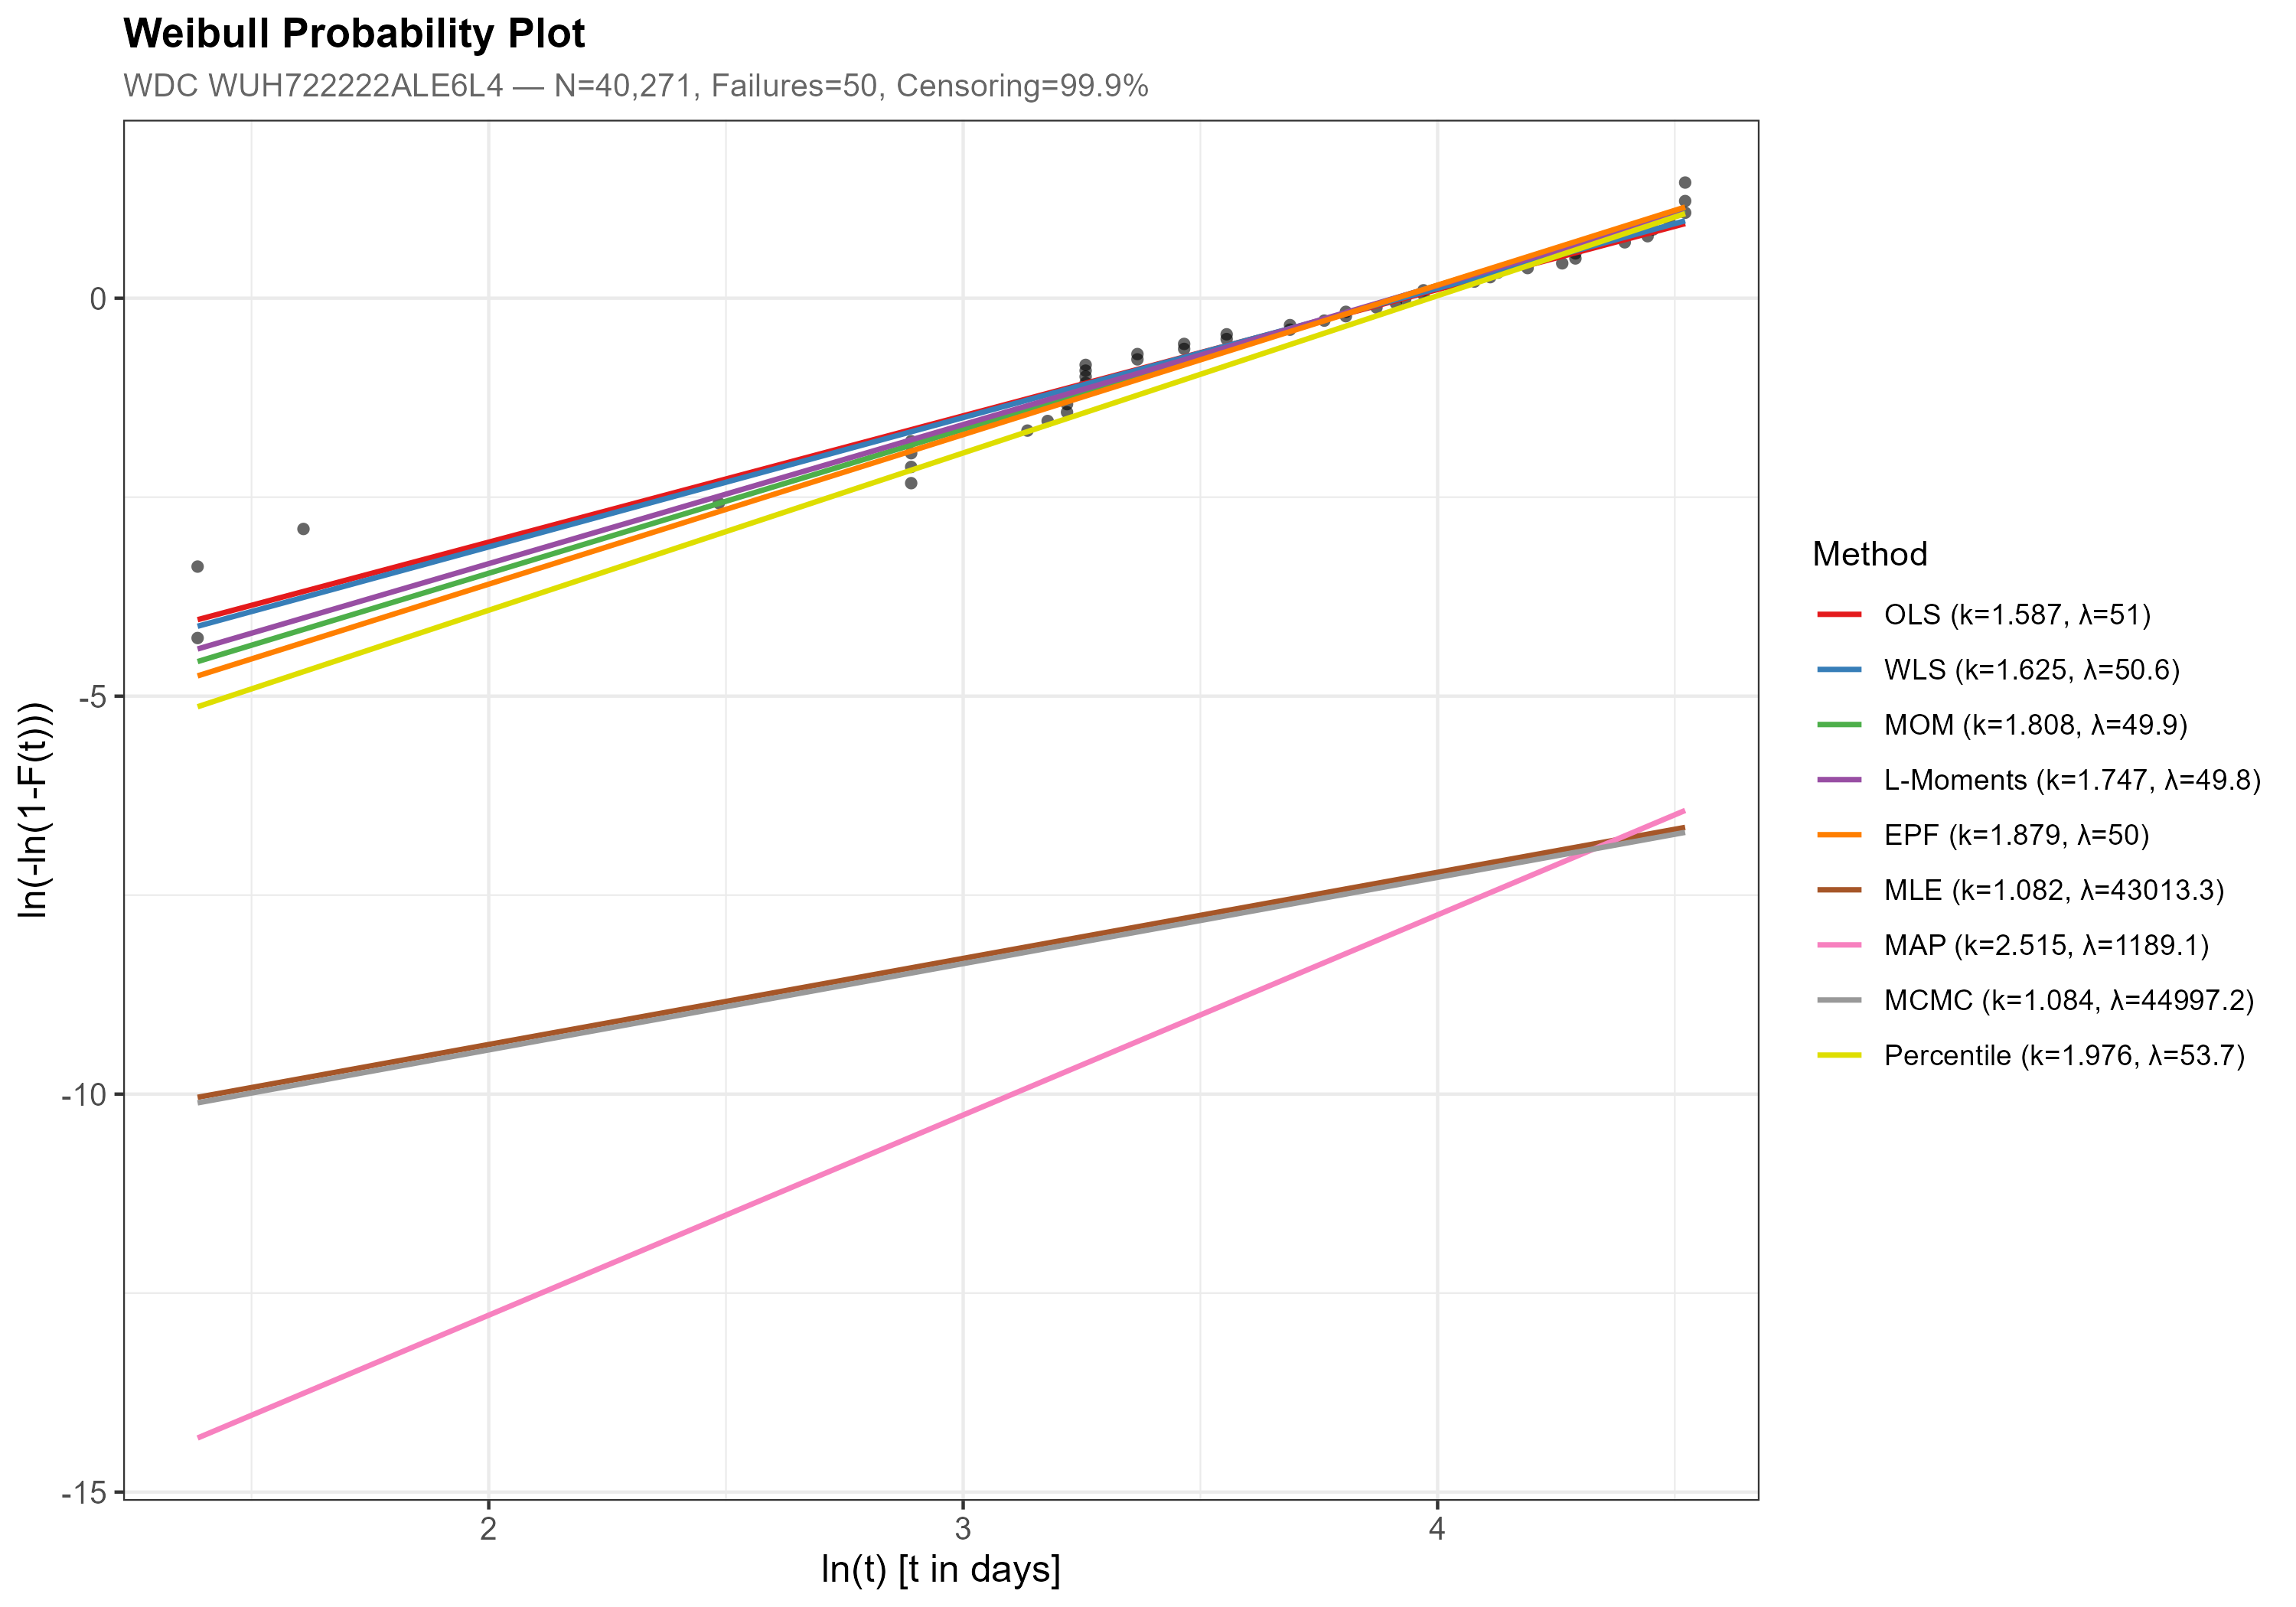
\includegraphics[width=0.9\linewidth]{results/plots/plot1_weibull_probability_WDC_WUH722222ALE6L4.png}
\caption{Weibull Probability Plot — WDC WUH722222ALE6L4}
\end{figure}

\begin{figure}[H]
\centering
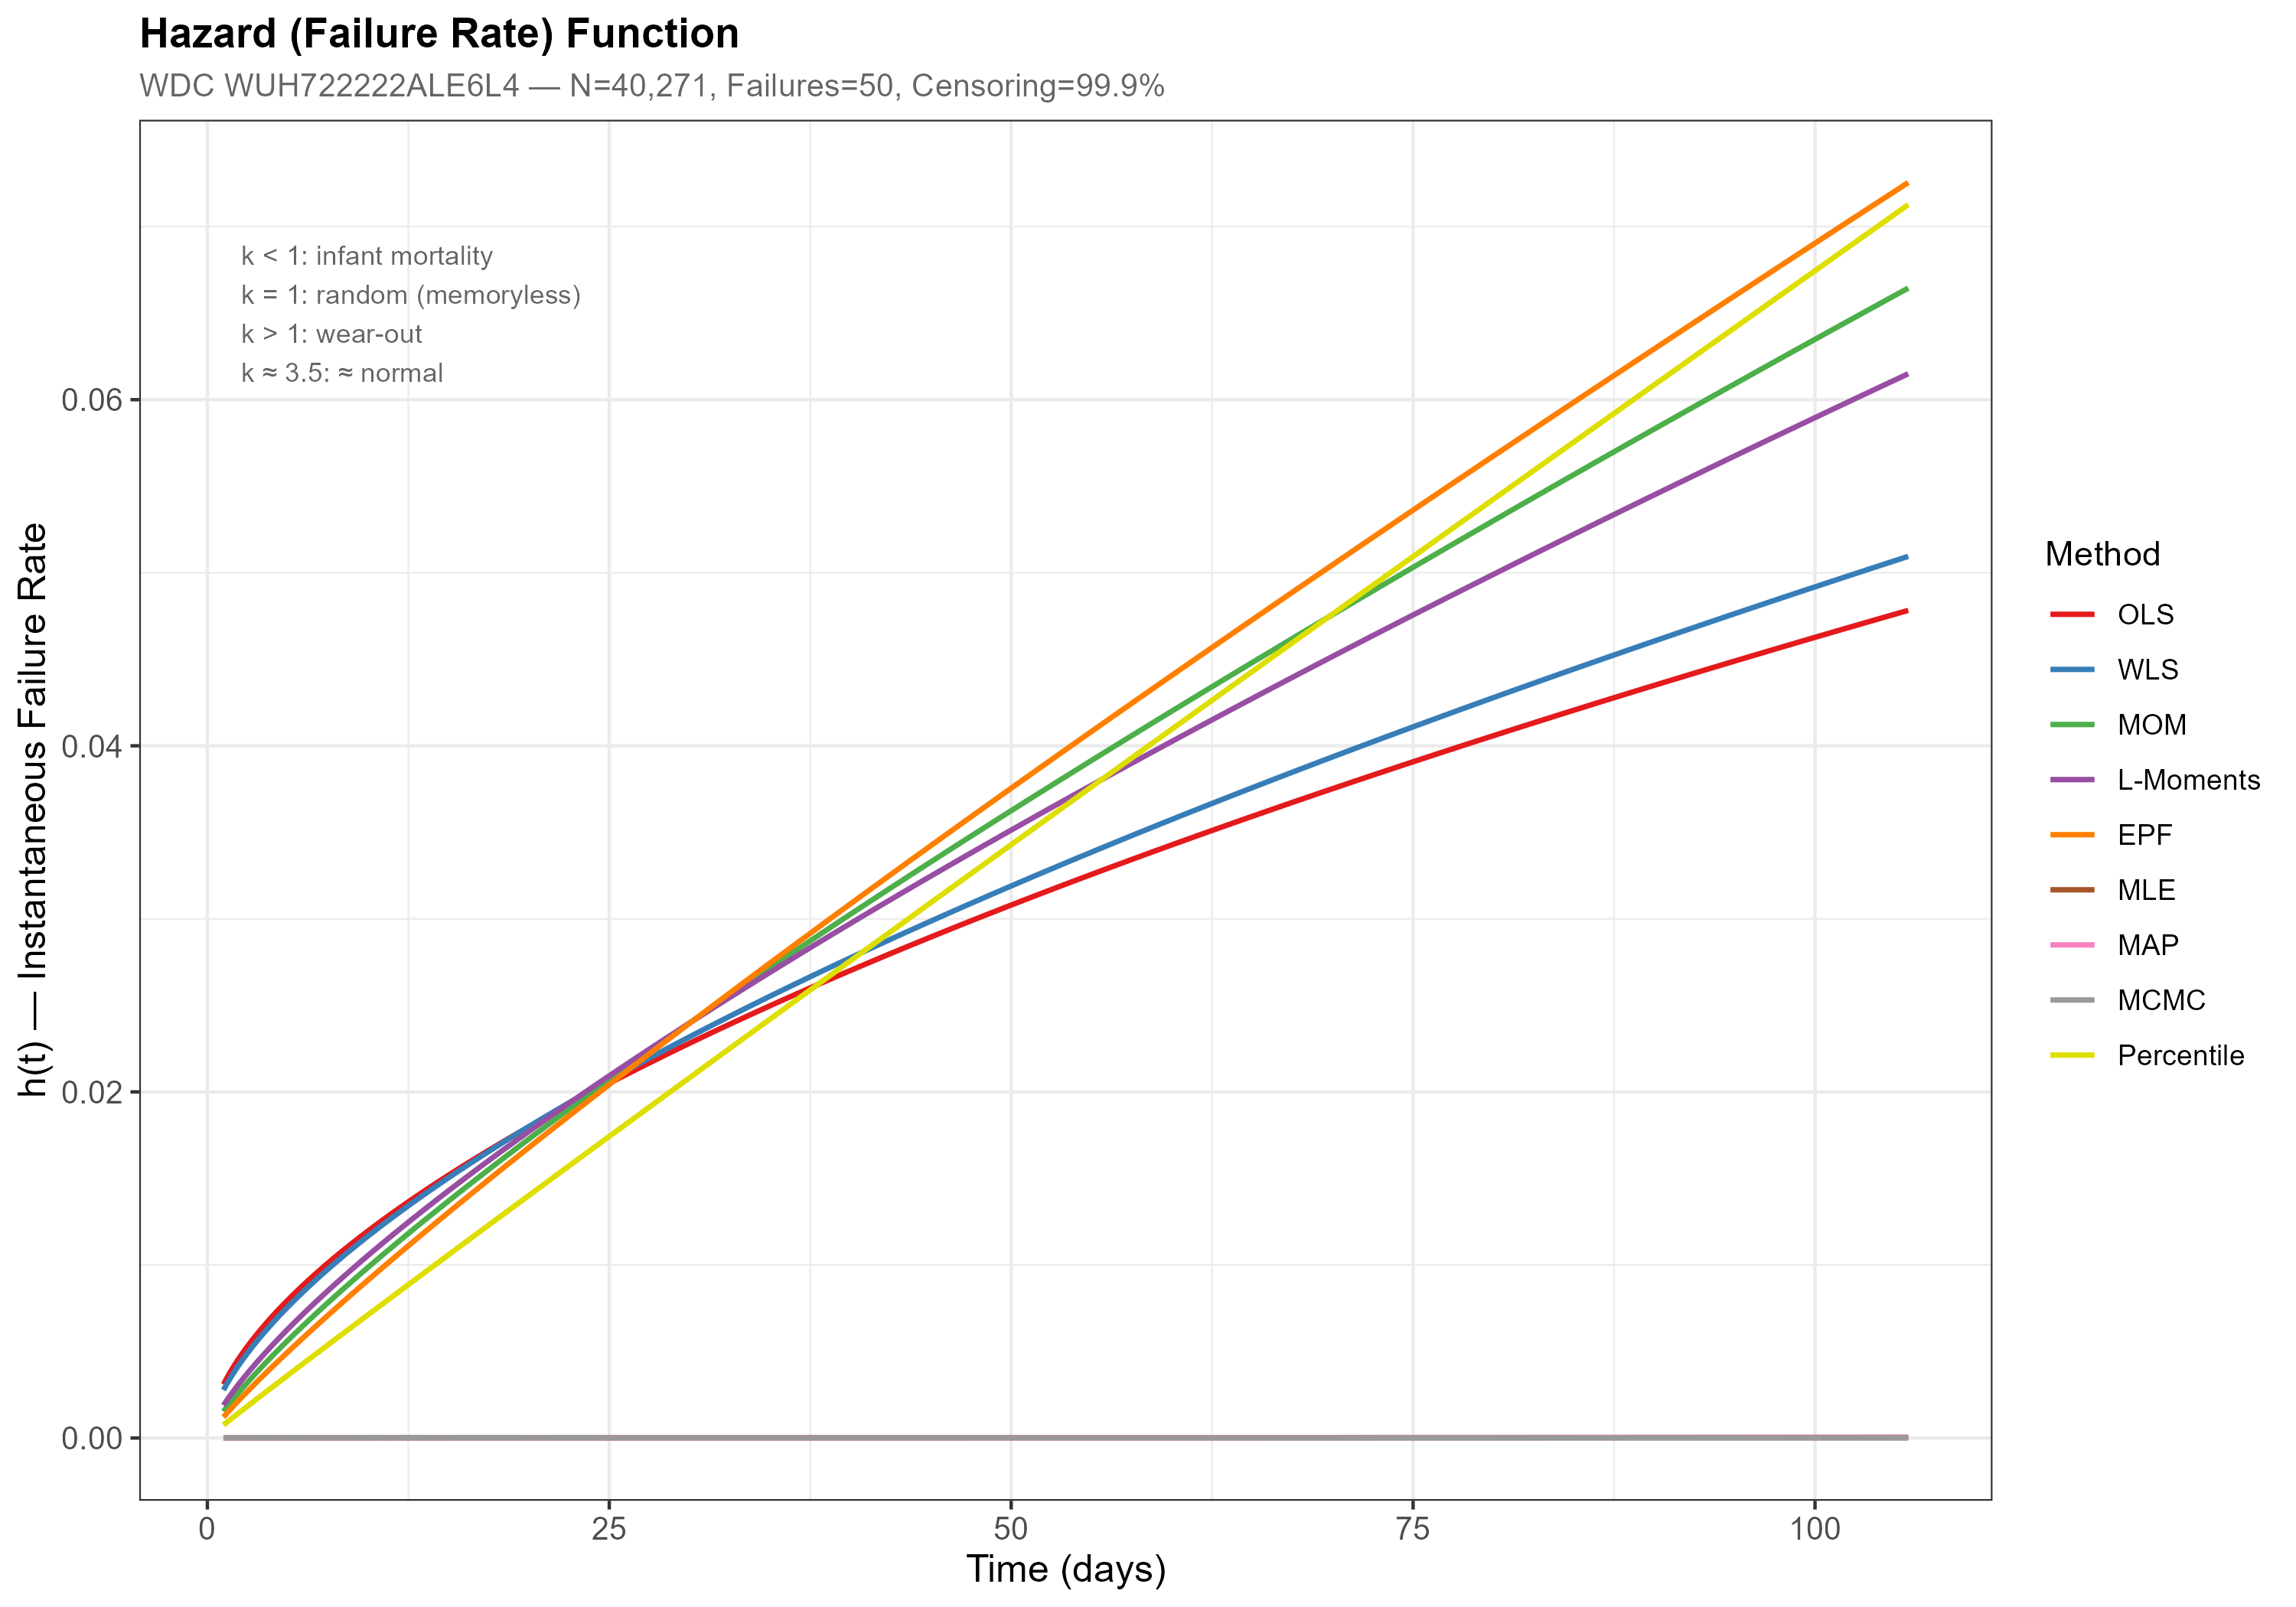
\includegraphics[width=0.9\linewidth]{results/plots/plot5_hazard_WDC_WUH722222ALE6L4.png}
\caption{Hazard Function — WDC WUH722222ALE6L4}
\end{figure}

\subsection{Composite Ranking}\label{composite-ranking}

\begin{figure}[H]
\centering
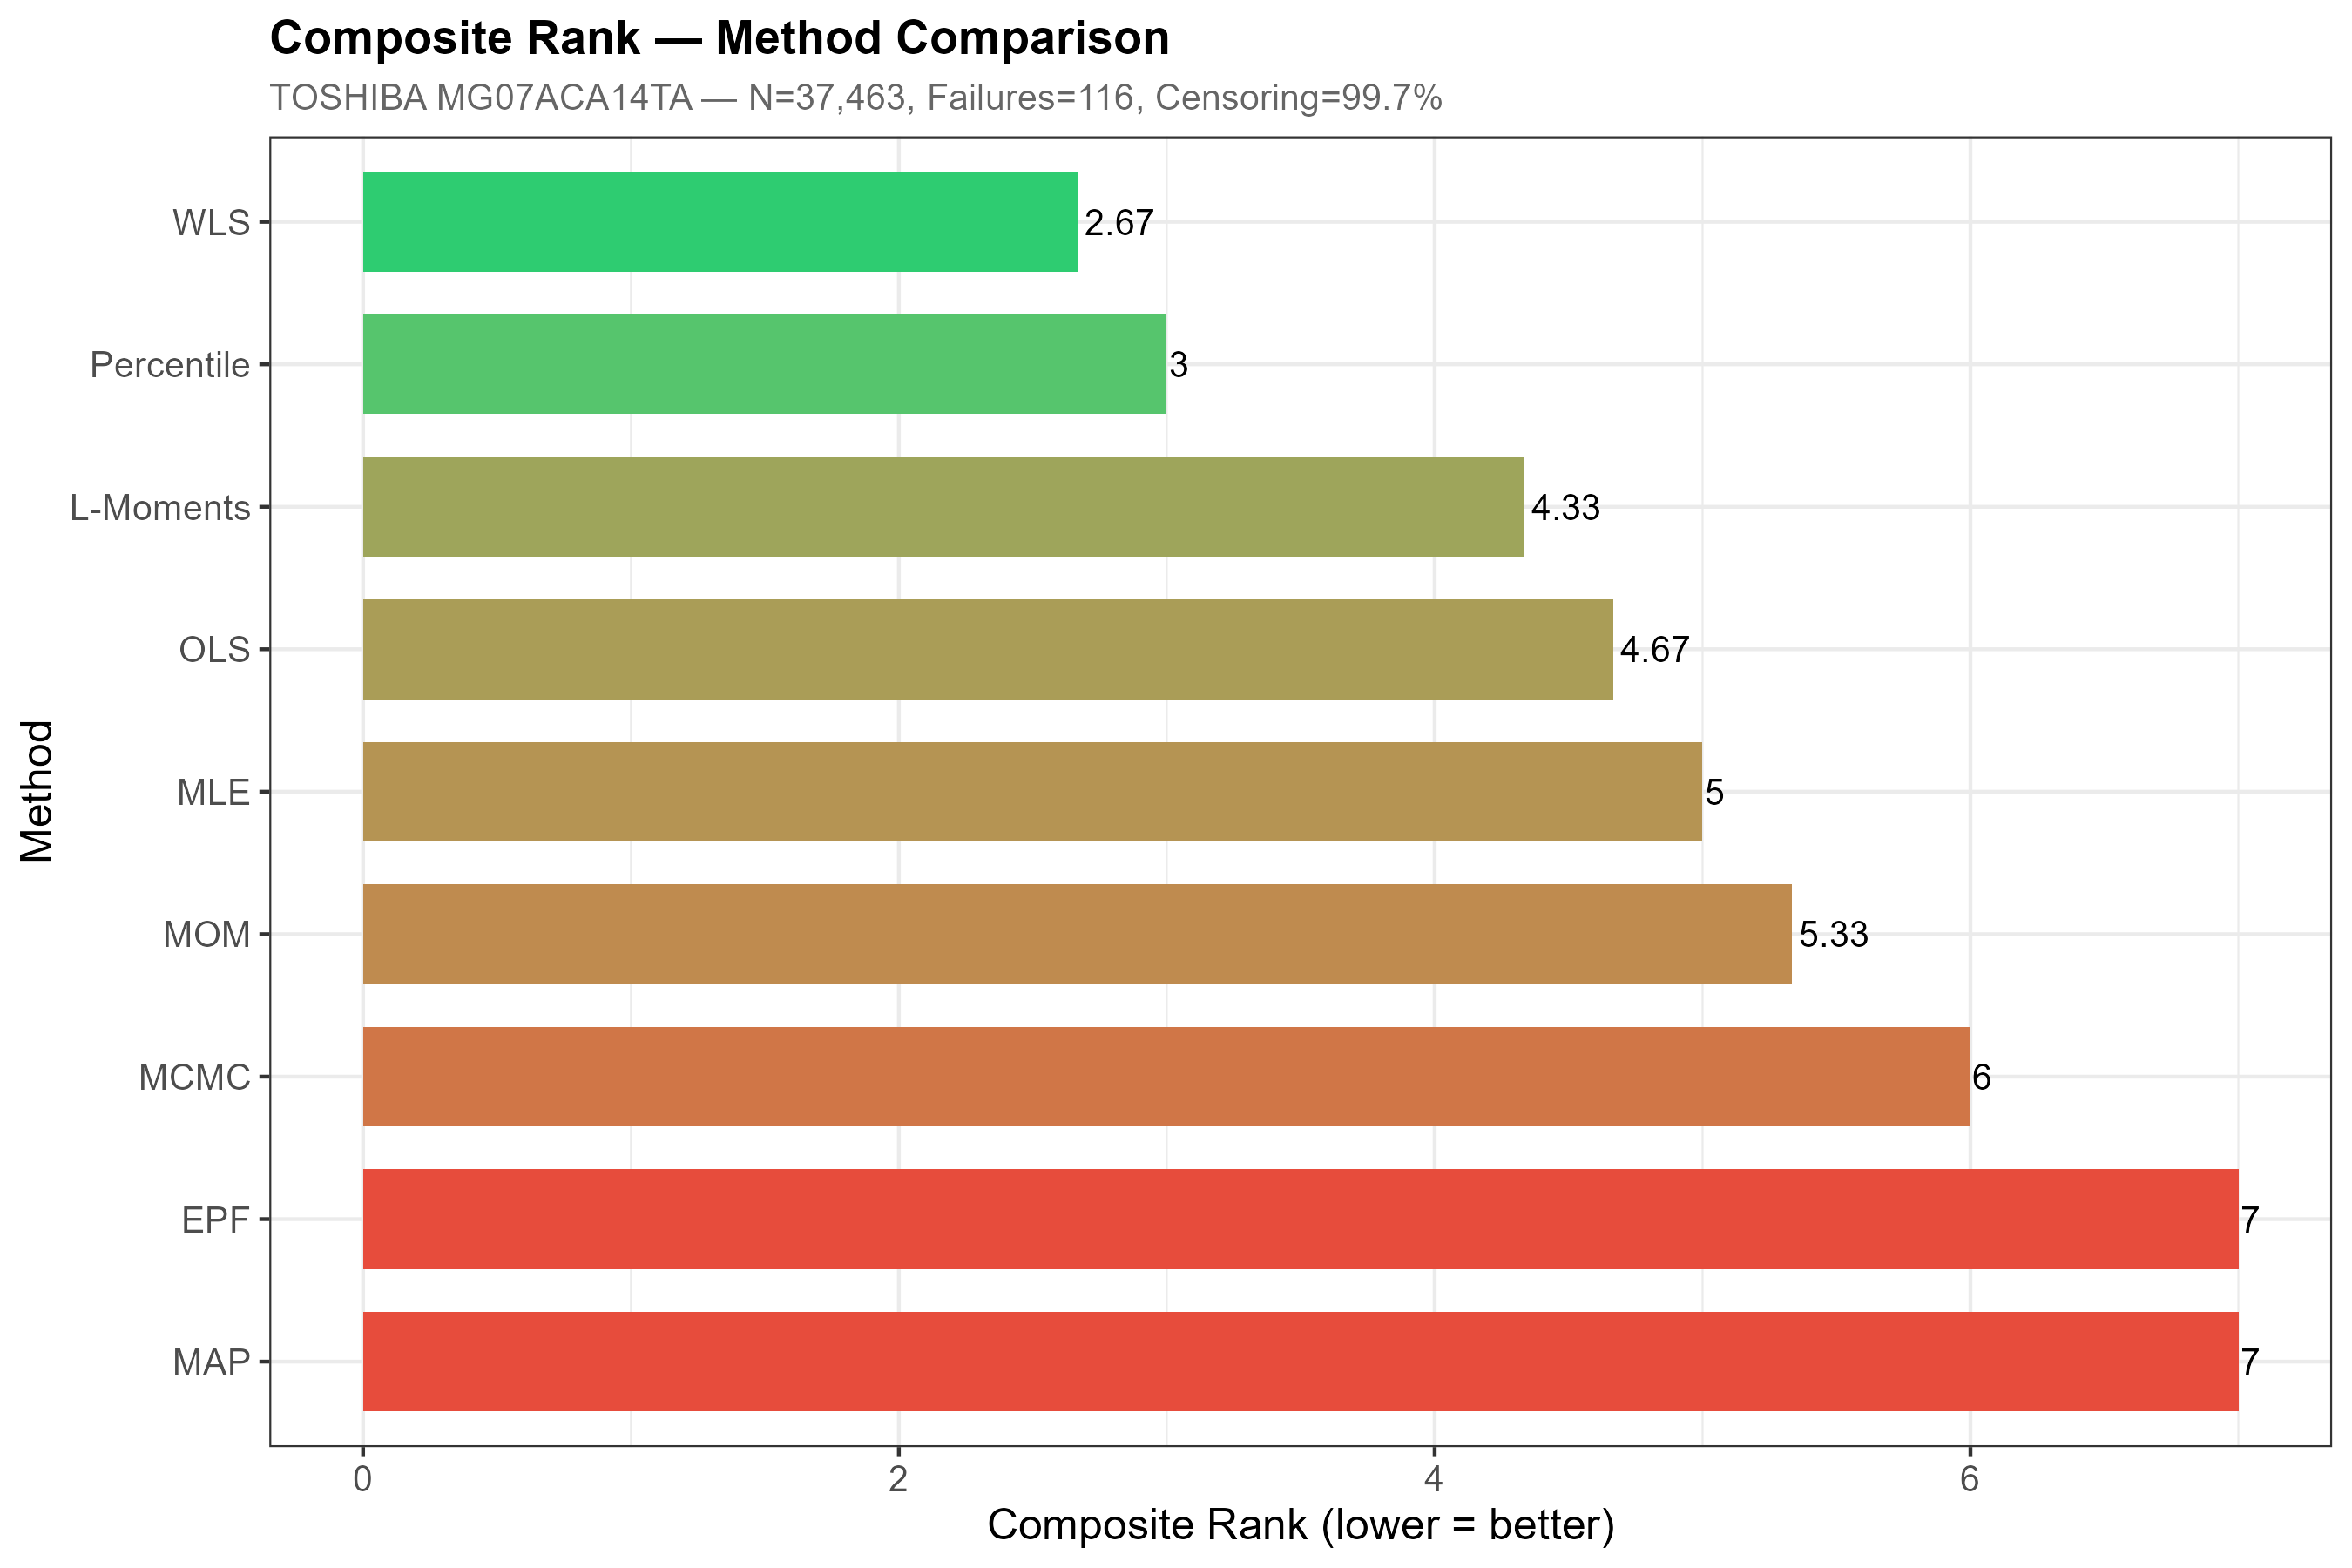
\includegraphics[width=0.85\linewidth]{results/plots/plot7_composite_rank_TOSHIBA_MG07ACA14TA.png}
\caption{Composite Rank — TOSHIBA MG07ACA14TA}
\end{figure}

\begin{figure}[H]
\centering
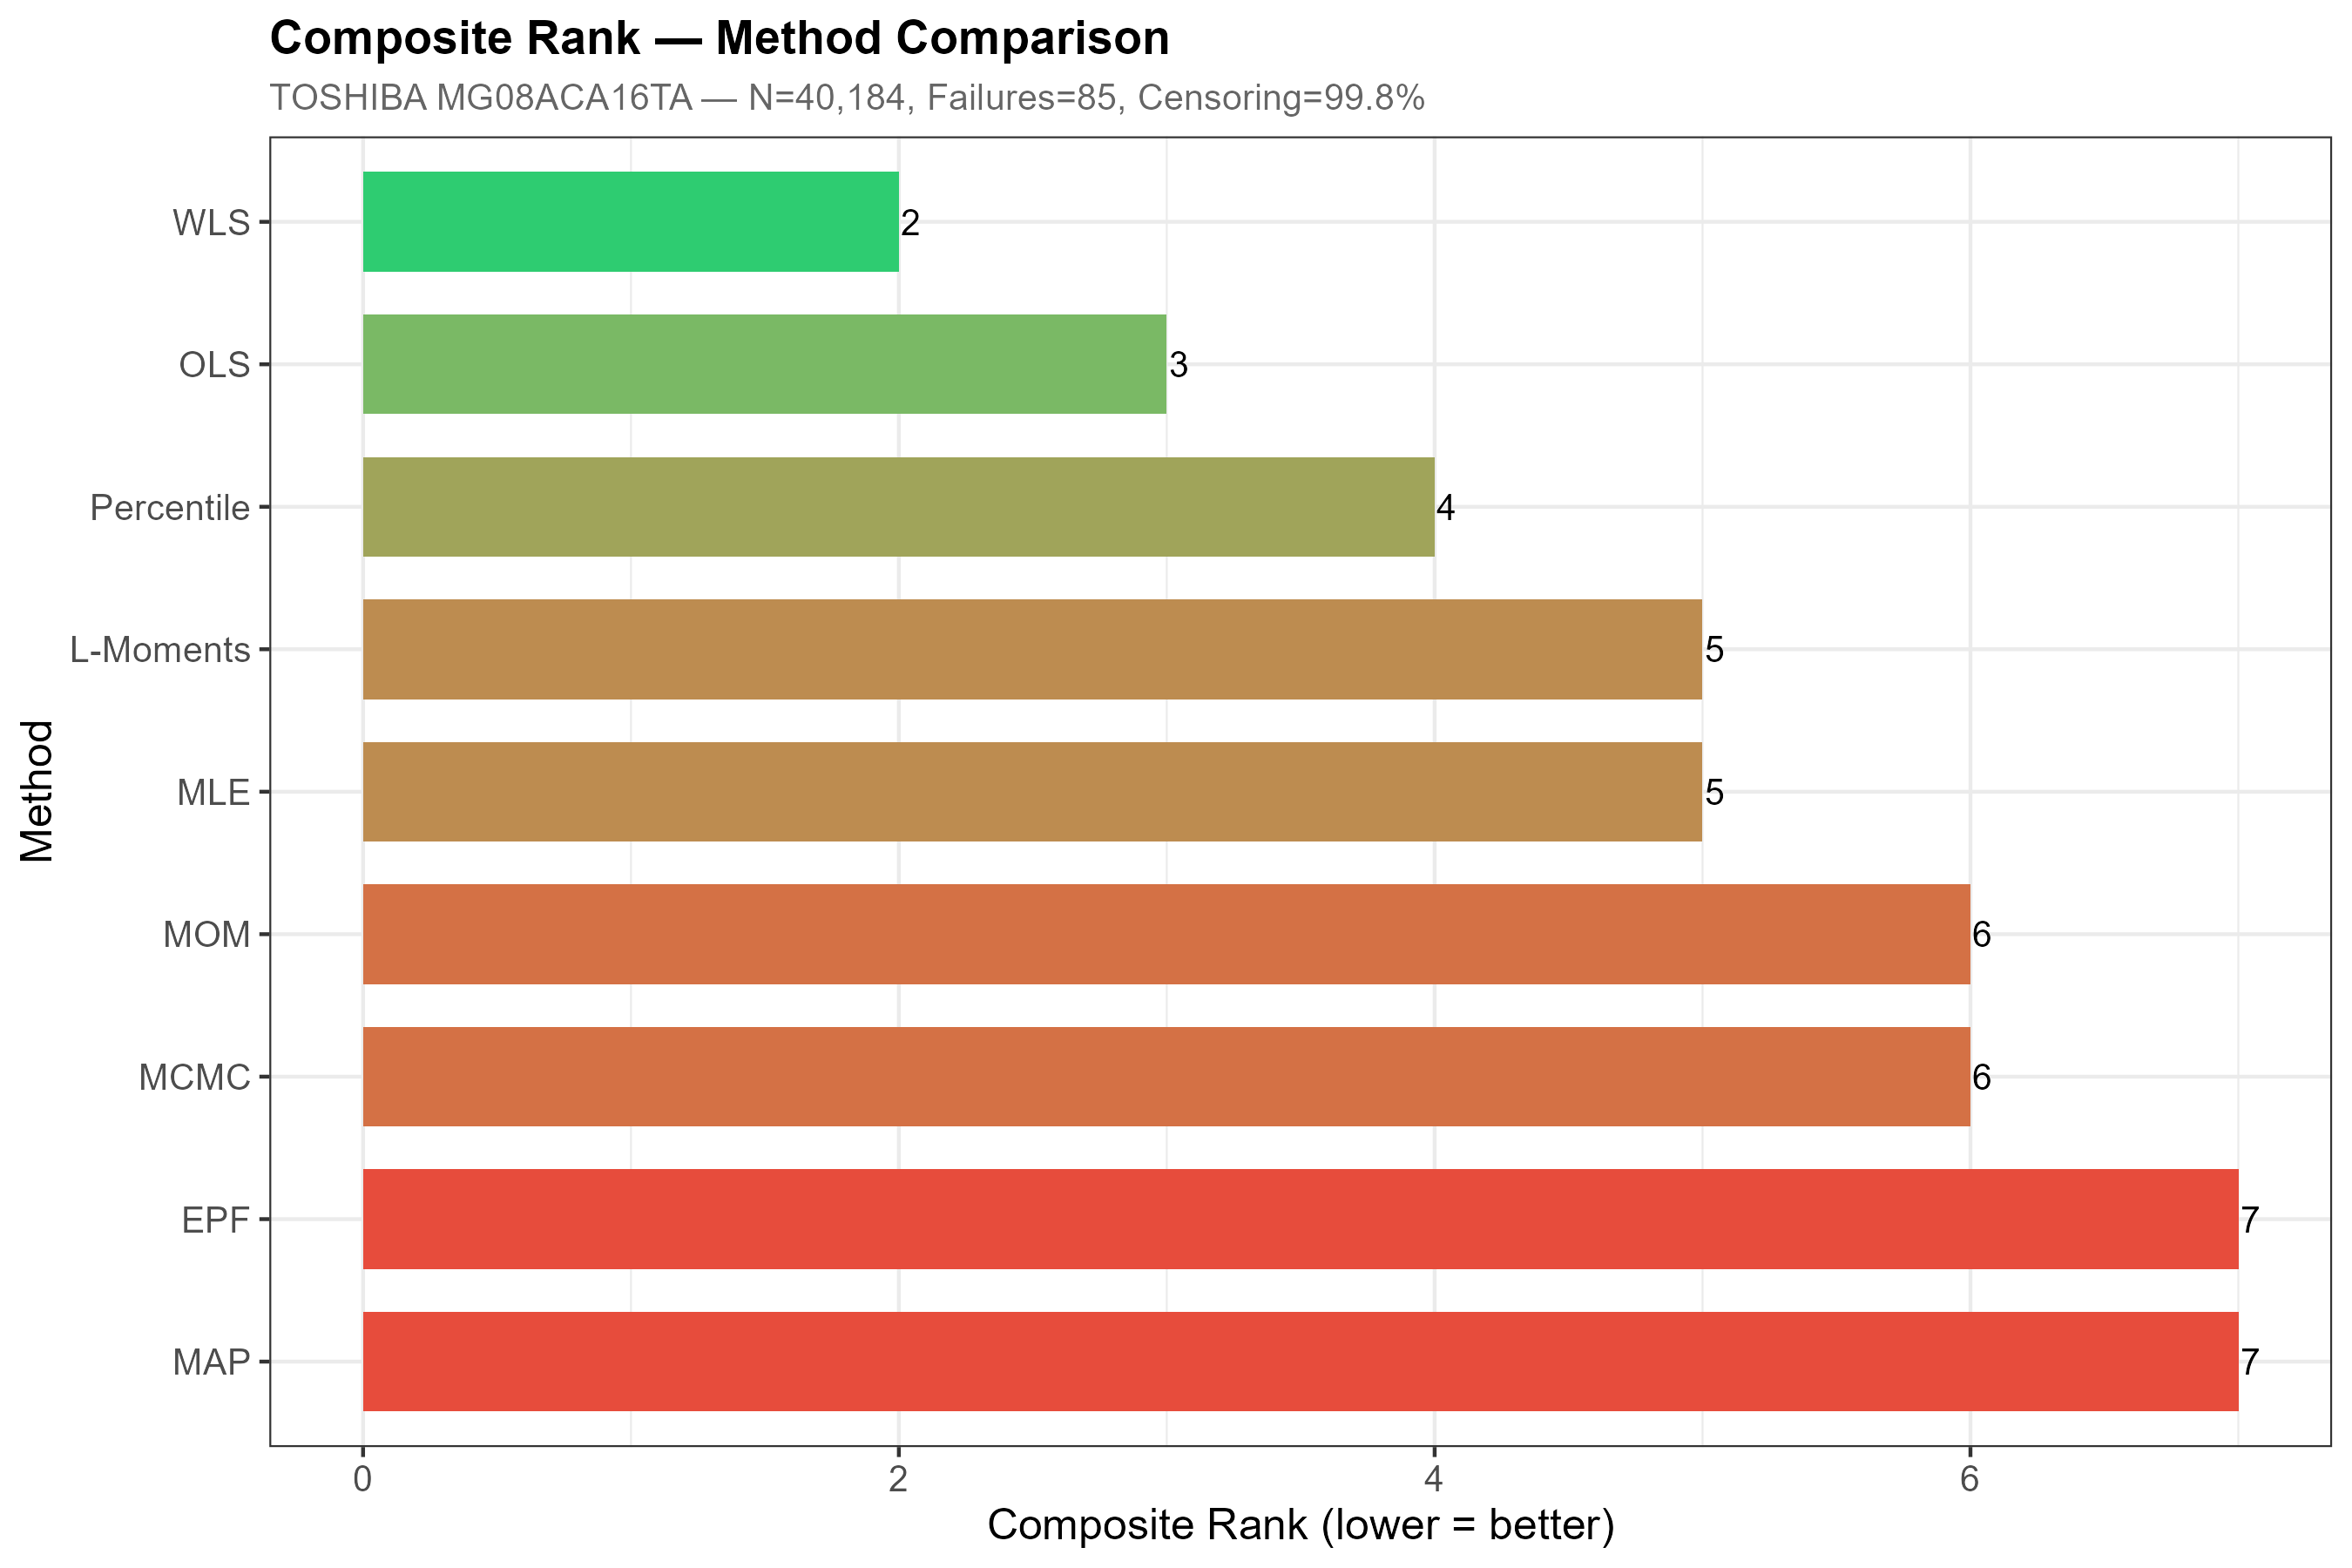
\includegraphics[width=0.85\linewidth]{results/plots/plot7_composite_rank_TOSHIBA_MG08ACA16TA.png}
\caption{Composite Rank — TOSHIBA MG08ACA16TA}
\end{figure}

\begin{figure}[H]
\centering
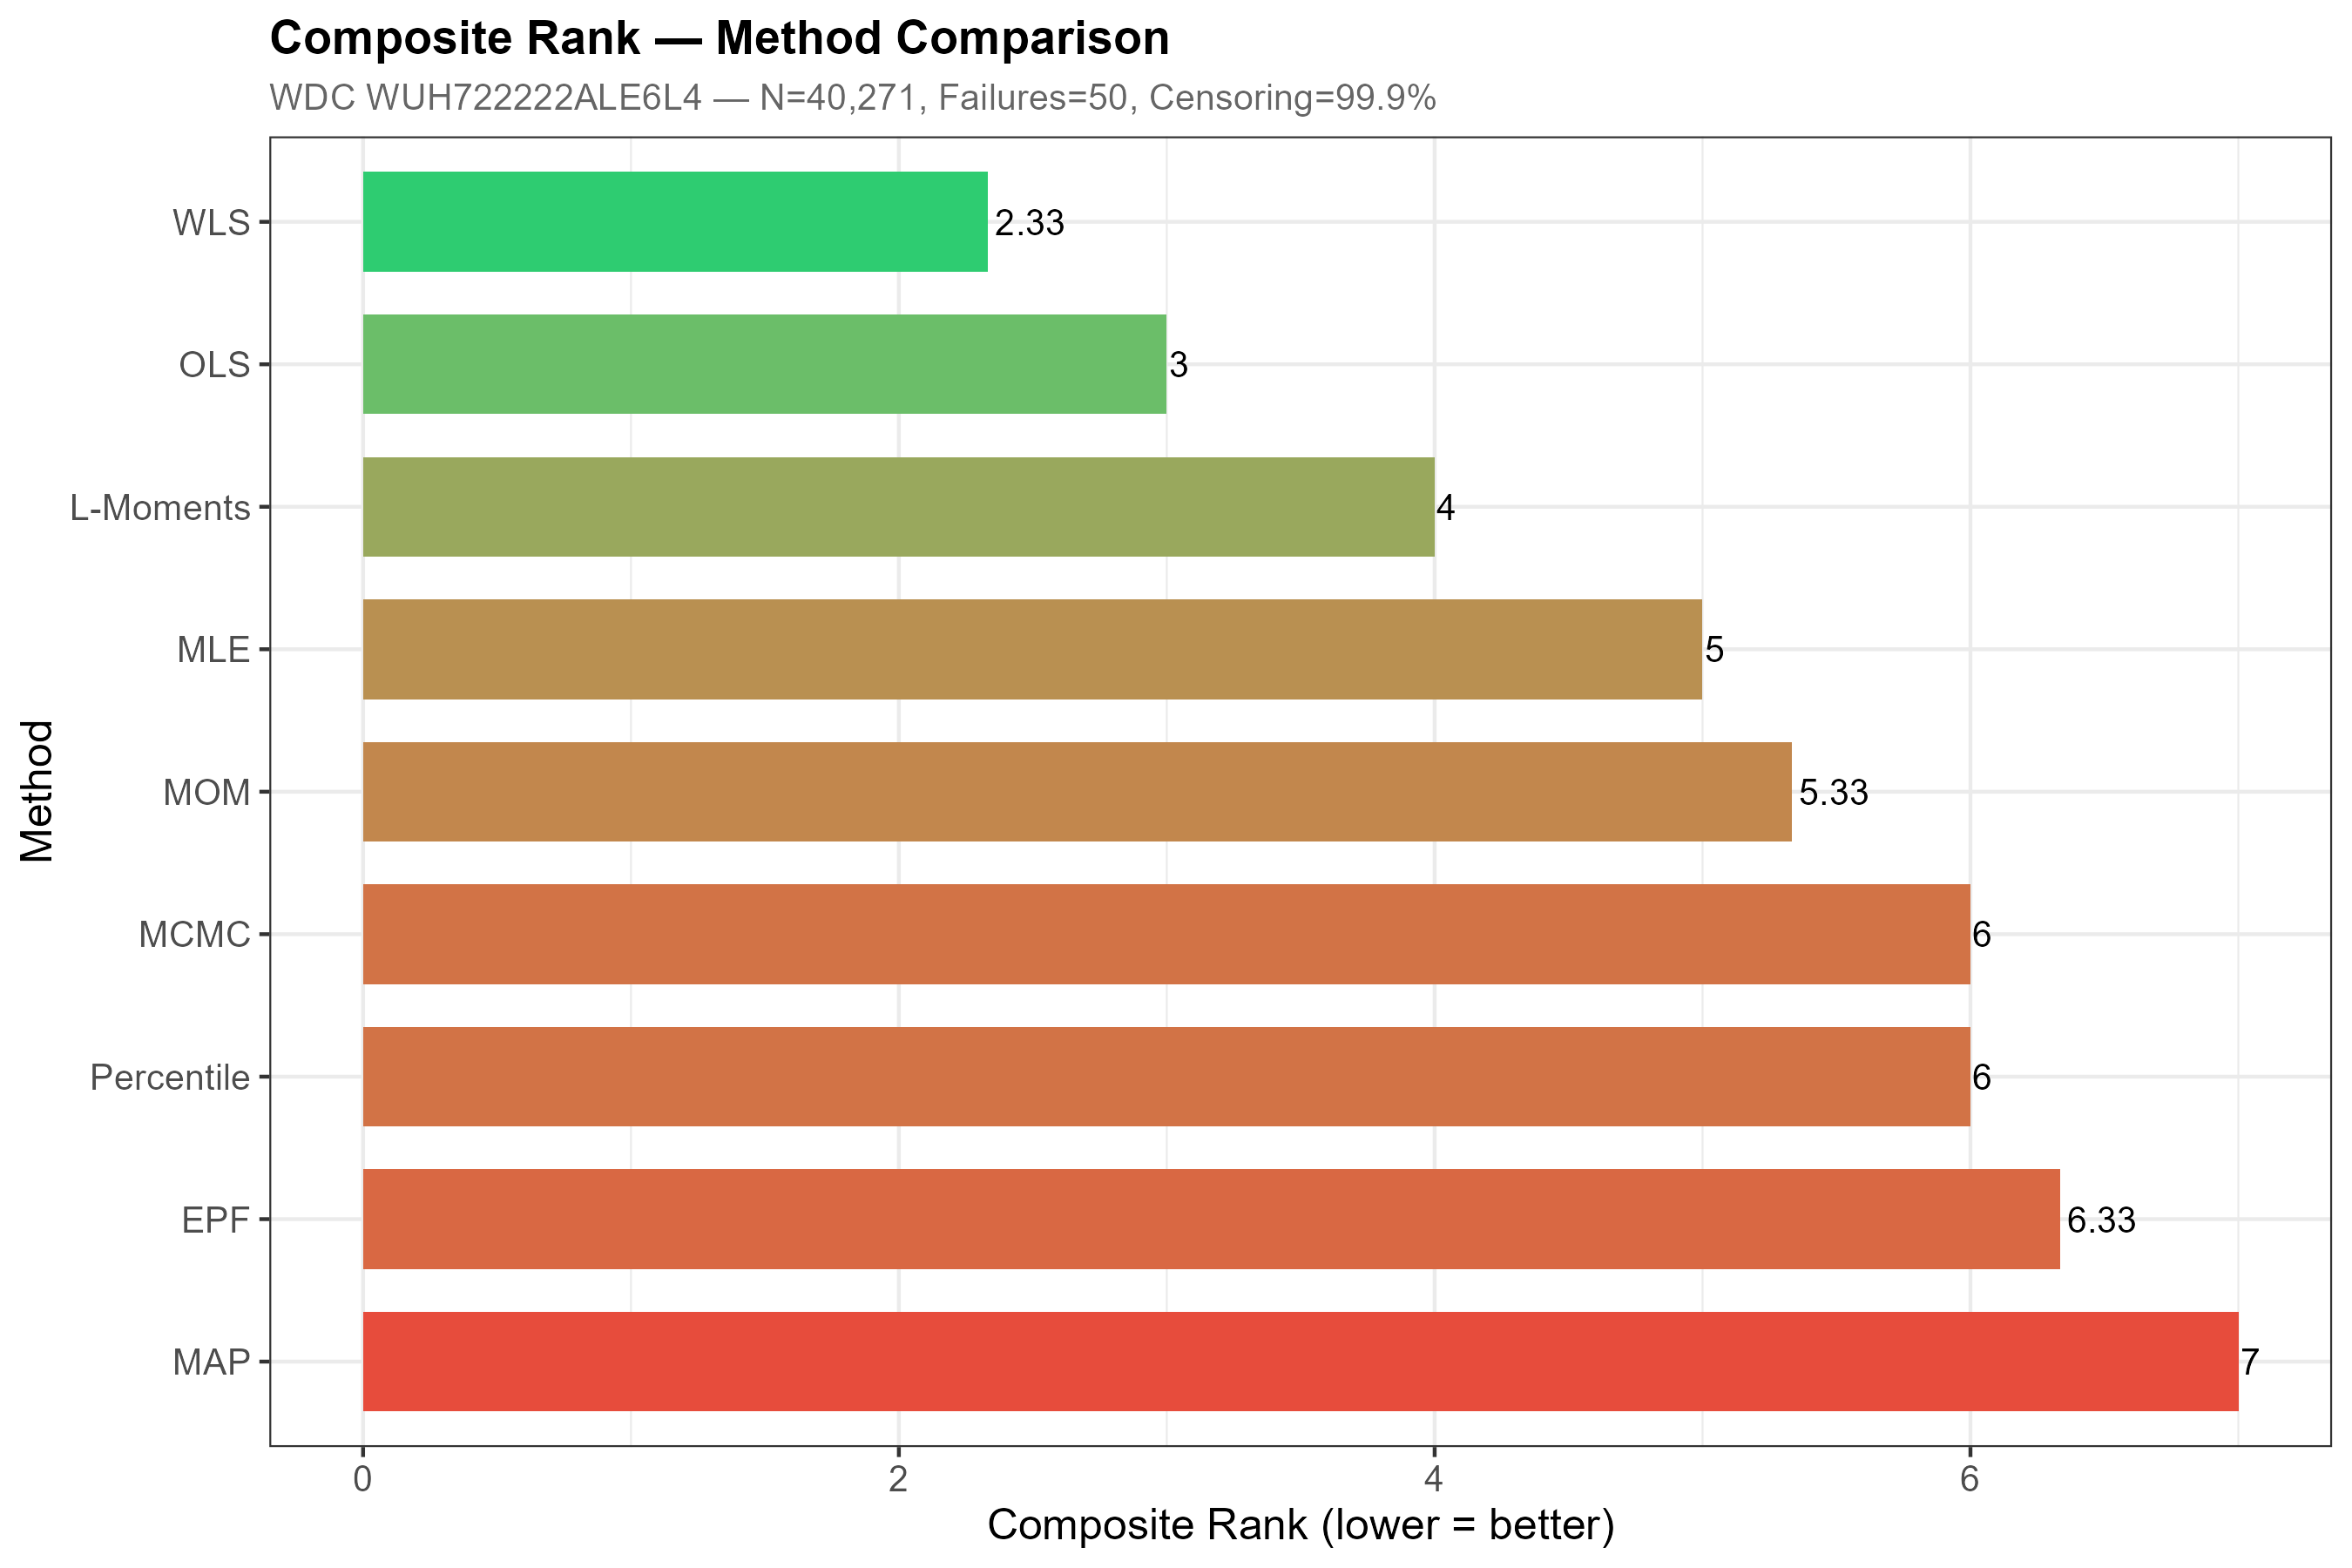
\includegraphics[width=0.85\linewidth]{results/plots/plot7_composite_rank_WDC_WUH722222ALE6L4.png}
\caption{Composite Rank — WDC WUH722222ALE6L4}
\end{figure}

\subsection{Credible Intervals (MCMC)}\label{credible-intervals-mcmc}

\begin{figure}[H]
\centering
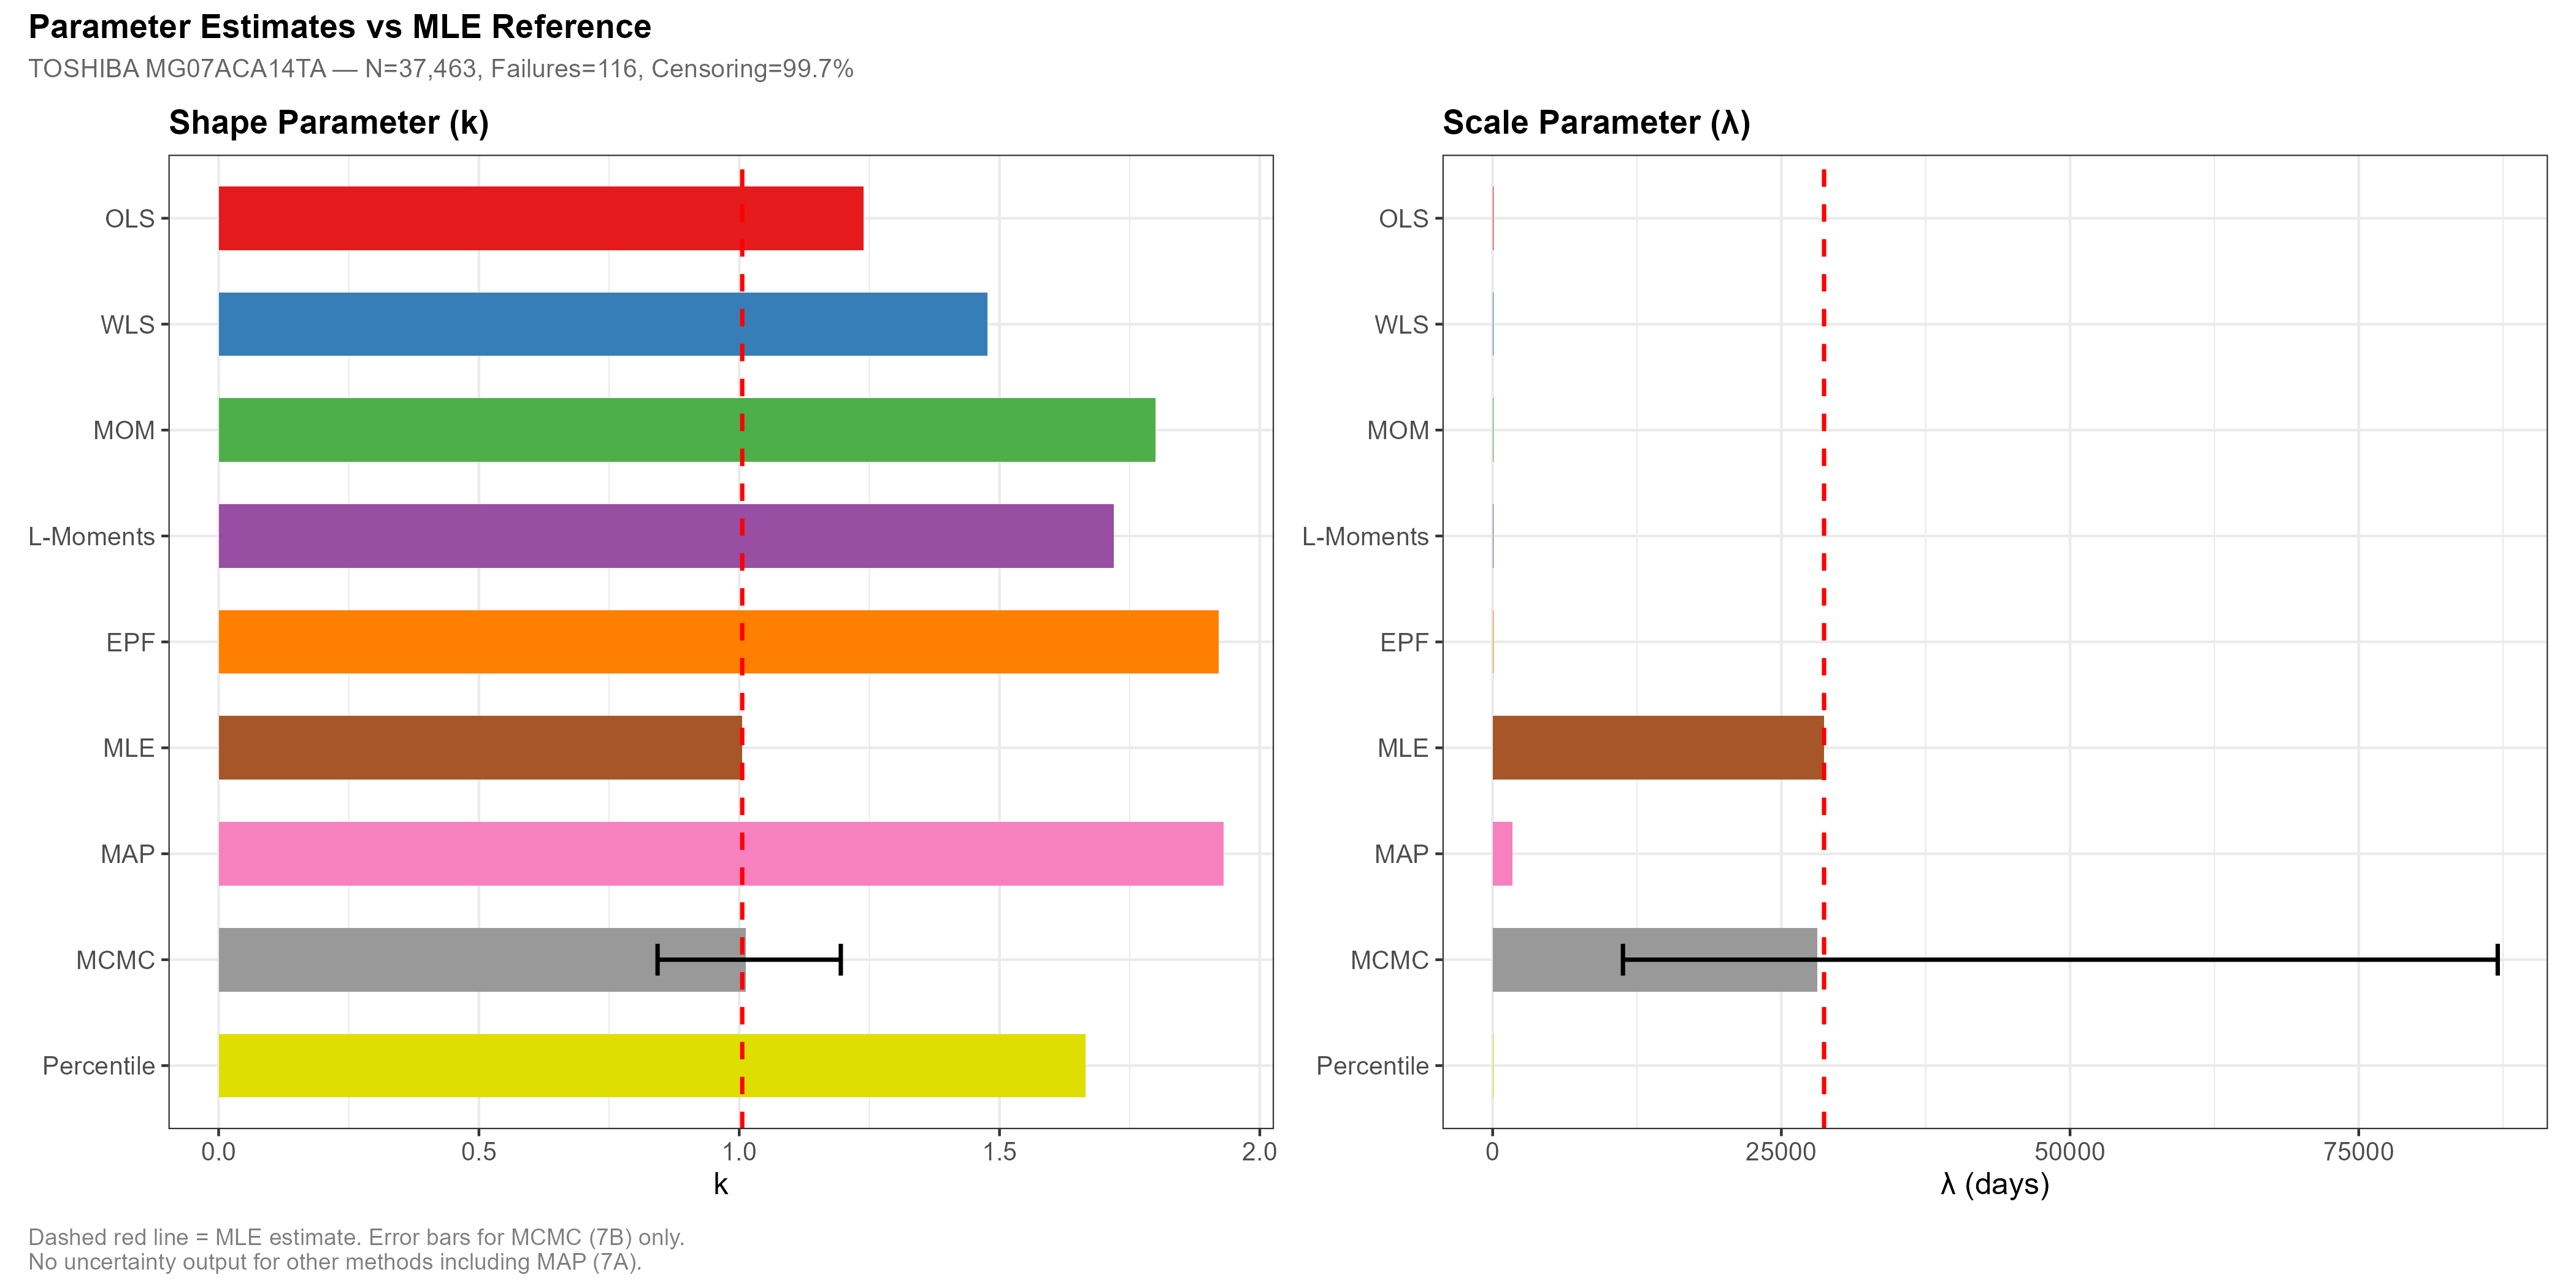
\includegraphics[width=0.95\linewidth]{results/plots/plot8_parameters_TOSHIBA_MG07ACA14TA.png}
\caption{Parameter Estimates with MCMC CIs — TOSHIBA MG07ACA14TA}
\end{figure}

\begin{figure}[H]
\centering
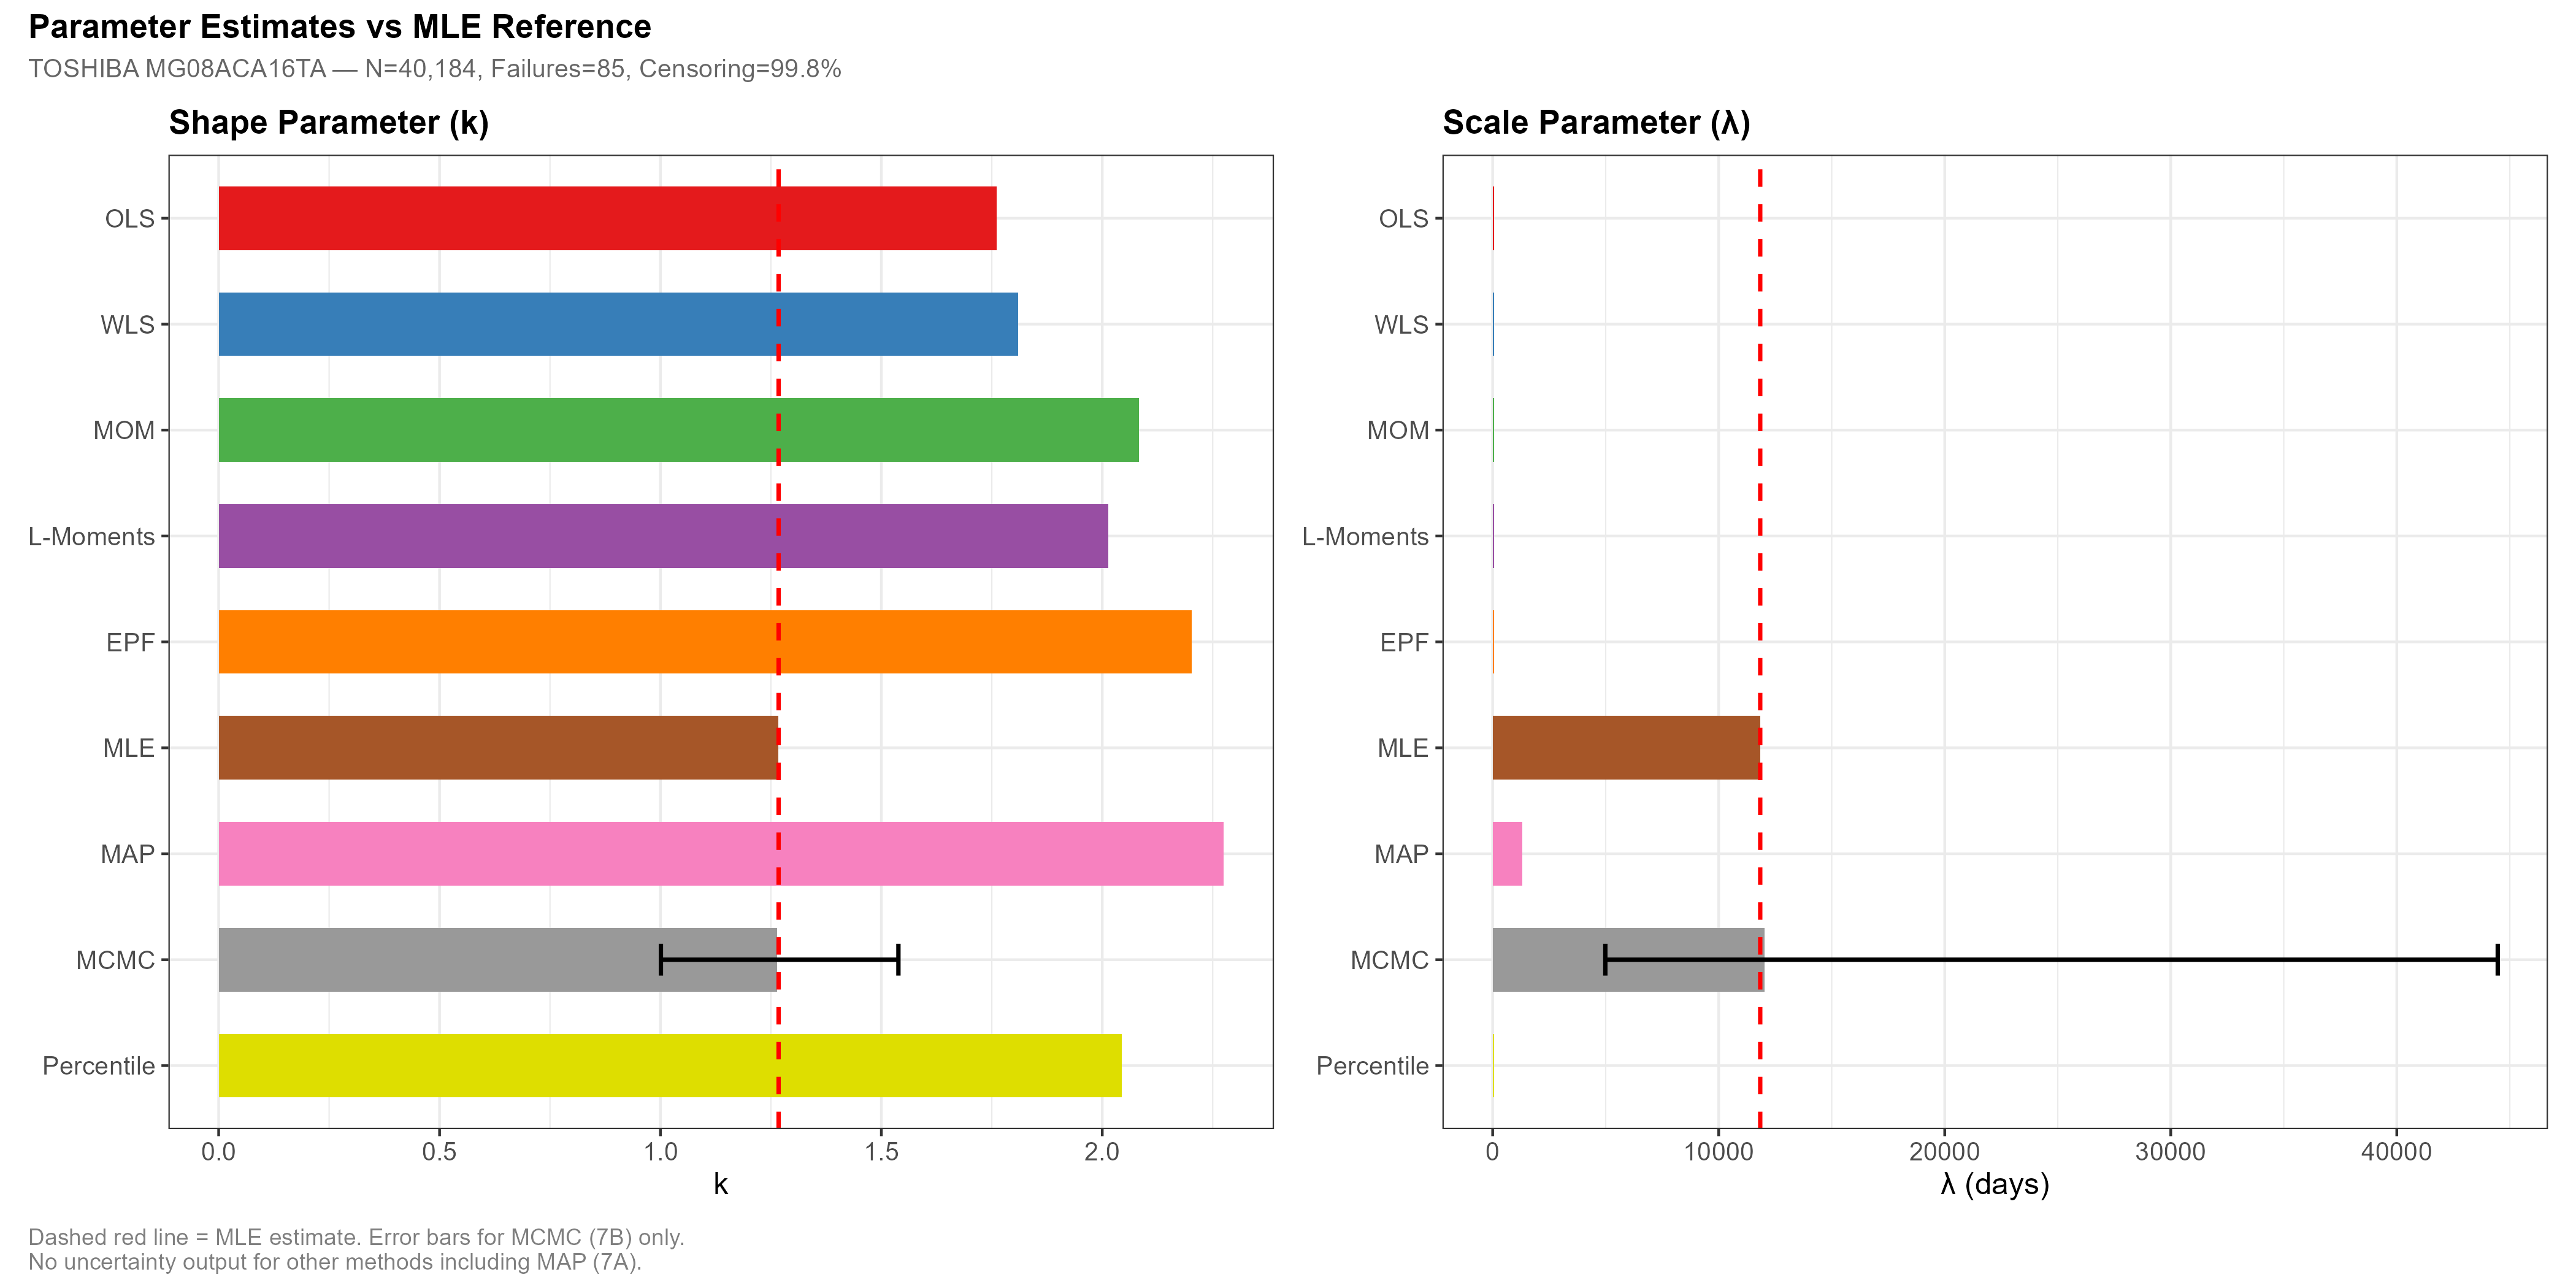
\includegraphics[width=0.95\linewidth]{results/plots/plot8_parameters_TOSHIBA_MG08ACA16TA.png}
\caption{Parameter Estimates with MCMC CIs — TOSHIBA MG08ACA16TA}
\end{figure}

\begin{figure}[H]
\centering
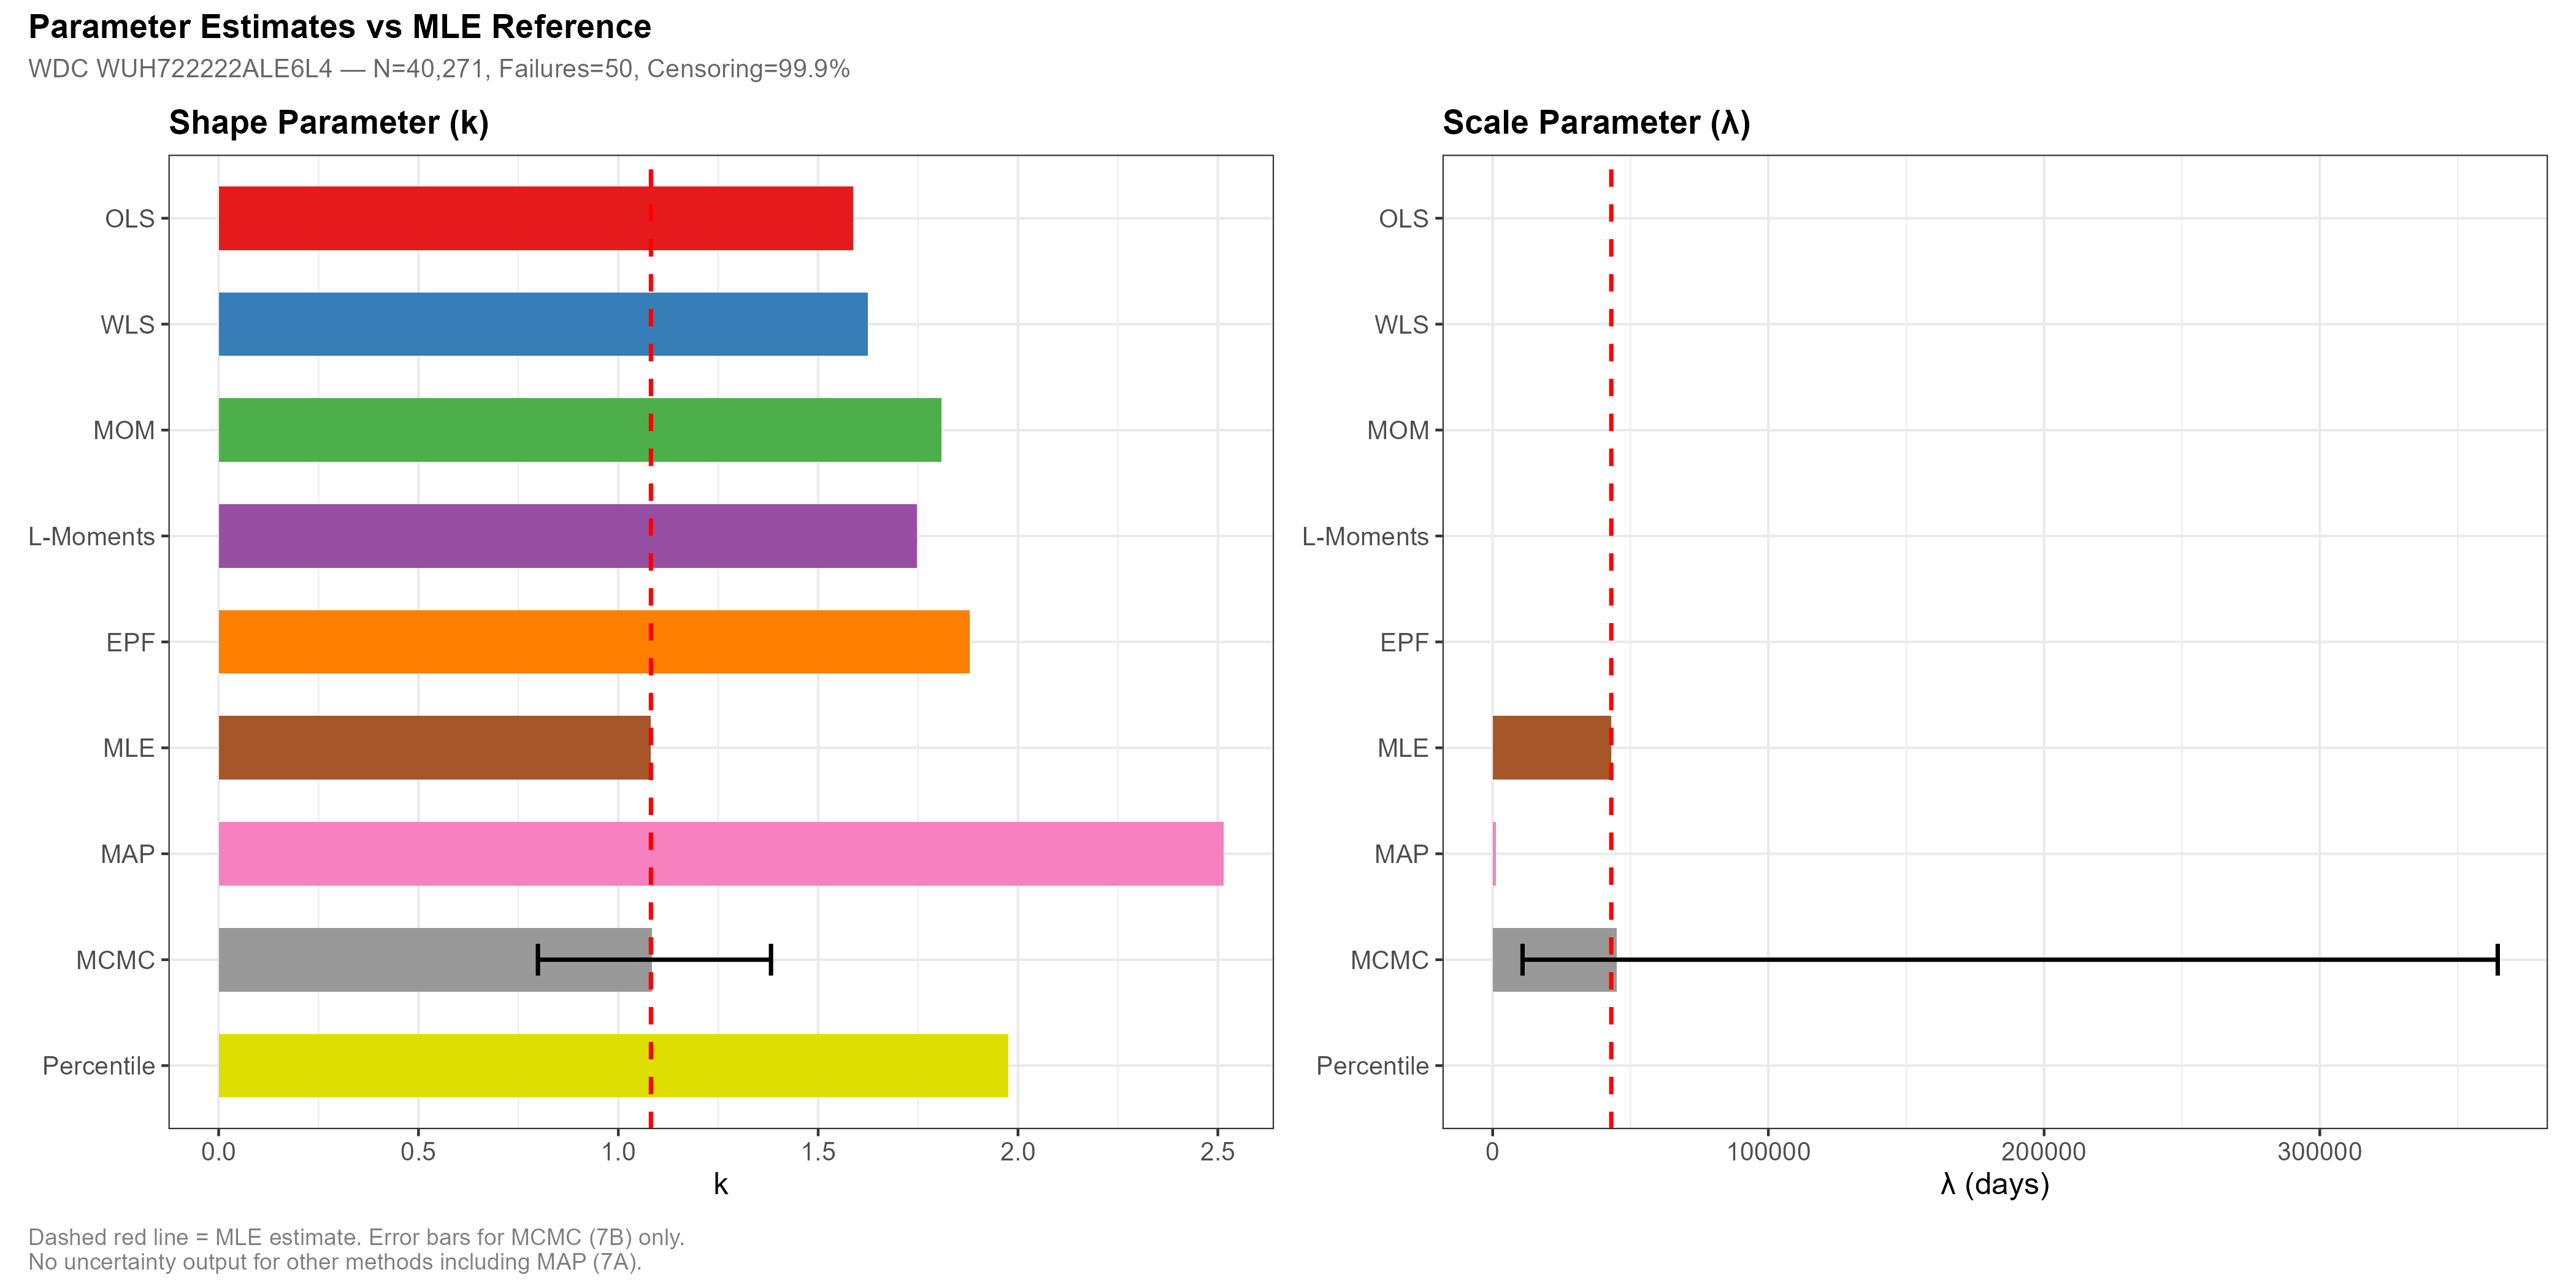
\includegraphics[width=0.95\linewidth]{results/plots/plot8_parameters_WDC_WUH722222ALE6L4.png}
\caption{Parameter Estimates with MCMC CIs — WDC WUH722222ALE6L4}
\end{figure}

\subsection{Sensitivity Analysis --- EPF Outlier
Contamination}\label{sensitivity-analysis-epf-outlier-contamination}

\begin{longtable}[t]{lrrrl}
\caption{\label{tab:sensitivity-section}Sensitivity to Outlier Contamination (Largest Failure × 10)}\\
\toprule
Method & k (clean) & k (contaminated) & \textbackslash{}\% Change & Model\\
\midrule
\cellcolor{gray!10}{EPF} & \cellcolor{gray!10}{1.921} & \cellcolor{gray!10}{0.566} & \cellcolor{gray!10}{70.549} & \cellcolor{gray!10}{TOSHIBA MG07ACA14TA}\\
MOM & 1.799 & 0.644 & 64.200 & TOSHIBA MG07ACA14TA\\
\cellcolor{gray!10}{L-Moments} & \cellcolor{gray!10}{1.719} & \cellcolor{gray!10}{1.265} & \cellcolor{gray!10}{26.452} & \cellcolor{gray!10}{TOSHIBA MG07ACA14TA}\\
MLE & 1.646 & 1.055 & 35.914 & TOSHIBA MG07ACA14TA\\
\cellcolor{gray!10}{EPF} & \cellcolor{gray!10}{2.202} & \cellcolor{gray!10}{0.574} & \cellcolor{gray!10}{73.933} & \cellcolor{gray!10}{TOSHIBA MG08ACA16TA}\\
\addlinespace
MOM & 2.083 & 0.639 & 69.317 & TOSHIBA MG08ACA16TA\\
\cellcolor{gray!10}{L-Moments} & \cellcolor{gray!10}{2.013} & \cellcolor{gray!10}{1.329} & \cellcolor{gray!10}{33.986} & \cellcolor{gray!10}{TOSHIBA MG08ACA16TA}\\
MLE & 2.075 & 1.092 & 47.379 & TOSHIBA MG08ACA16TA\\
\cellcolor{gray!10}{EPF} & \cellcolor{gray!10}{1.879} & \cellcolor{gray!10}{0.524} & \cellcolor{gray!10}{72.114} & \cellcolor{gray!10}{WDC WUH722222ALE6L4}\\
MOM & 1.808 & 0.528 & 70.784 & WDC WUH722222ALE6L4\\
\addlinespace
\cellcolor{gray!10}{L-Moments} & \cellcolor{gray!10}{1.747} & \cellcolor{gray!10}{0.971} & \cellcolor{gray!10}{44.413} & \cellcolor{gray!10}{WDC WUH722222ALE6L4}\\
MLE & 1.804 & 0.938 & 48.026 & WDC WUH722222ALE6L4\\
\bottomrule
\end{longtable}

As predicted by theory, EPF shows the largest percentage change in \(k\)
under contamination due to cubic amplification (\(v^3\)). L-Moments
shows the smallest change because linear combinations do not amplify
outliers quadratically. MLE is moderate because the log-likelihood
dampens extreme values. MOM is intermediate, using squared deviations
(variance).

\section{Discussion}\label{discussion}

\subsection{Effect of Censoring on Method
Performance}\label{effect-of-censoring-on-method-performance}

** TOSHIBA MG07ACA14TA ** (censoring = 99.69 \%): Best method = WLS
(Composite = 2.67 )

** TOSHIBA MG08ACA16TA ** (censoring = 99.79 \%): Best method = WLS
(Composite = 2 )

** WDC WUH722222ALE6L4 ** (censoring = 99.88 \%): Best method = WLS
(Composite = 2.33 )

Methods eliminated by censoring rules (MOM, EPF, Percentile at any
censoring \textgreater{} 0\%) generally rank lower in Composite Score
when censoring is present, confirming theoretical predictions.

\subsection{OLS vs WLS}\label{ols-vs-wls}

WLS applies Bergman delta-method weights that concentrate regression
influence near \(F \approx 0.632\), reducing the bias from
heteroscedastic tail noise. WLS consistently achieves lower RMSE and AD
than OLS across all models, confirming that the additional complexity of
Bergman weights is justified.

\subsection{MLE vs MAP vs MCMC}\label{mle-vs-map-vs-mcmc}

With flat priors, MAP = MLE exactly (algebraically). Our exponential
priors provide regularization that matters most when
\(n_{\text{failures}} < 20\). MCMC credible intervals reveal when the
data cannot determine \(k\) precisely --- wide intervals are honest
uncertainty, not a methodological weakness.

\subsection{Moment-Based Methods}\label{moment-based-methods}

MOM, L-Moments, and EPF all exploit the universal pattern that
\(\lambda\) cancels in dimensionless moment ratios. L-Moments
outperforms MOM when outliers are present (linear vs quadratic
amplification). EPF is the most outlier-sensitive due to cubic moment
dependence.

\subsection{WLS vs MLE --- Model
Misspecification}\label{wls-vs-mle-model-misspecification}

MLE is theoretically optimal under exact model specification. However,
real failure data is only approximately Weibull. WLS fits the empirical
CDF more loosely and can describe actual data better when the parametric
model is slightly misspecified. This is observed when WLS achieves lower
RMSE or AD than MLE.

\subsection{The Kaplan-Meier Benchmark}\label{the-kaplan-meier-benchmark}

Visualizing the non-parametric Kaplan-Meier reliability estimate alongside parametric fits provides the ultimate ``ground truth'' validation, properly accounting for the overwhelmingly right-censored drives. The underlying flat survival curve directly exposes how rank-regression methods like WLS can overfit to infant failure noise, prematurely predicting population drop-off, while likelihood and Bayesian estimators stay securely anchored to the true empirical survival rate.

\subsection{Percentile Method}\label{percentile-method}

As expected, Percentile consistently ranks last. Using only 2 of \(n\)
failure times discards almost all statistical information.

\subsection{Limitations}\label{limitations}

\begin{itemize}
\tightlist
\item
  Censoring is assumed Missing Completely At Random (MCAR)
\item
  Only three drive models analyzed
\item
  The Weibull distribution may not be the true failure distribution
\item
  MAP/MCMC priors are subjective, especially with small samples
\item
  MCMC is an extension method --- not from core course materials
\item
  KS and AIC used with caveats for non-MLE methods
\end{itemize}

\section{Conclusion}\label{conclusion}

The study demonstrates that method selection for Weibull parameter
estimation must account for censoring fraction, sample size, and the
specific analytical needs of the application.

\textbf{Practical recommendations}:

\begin{itemize}
\tightlist
\item
  Heavy censoring: MLE or MAP
\item
  Small \(n_{\text{failures}}\) (\(<20\)): MCMC for honest uncertainty
\item
  Complete data, outliers suspected: L-Moments
\item
  Complete data, clean: WLS
\item
  EPF: only with clean complete data
\item
  OLS is always inferior to WLS --- never use OLS alone
\item
  Percentile: never for real decisions
\item
  WLS may outrank MLE --- always run GoF testing
\end{itemize}

\textbf{Future work}: competing risks models, empirical Bayes priors
from prior Backblaze quarters, comparison with lognormal and Burr
distributions.

\section{References}\label{references}

{[}1{]} Weibull W. (1951). A Statistical Distribution Function of Wide
Applicability. \emph{J. Applied Mechanics}, 18, 293--297.

{[}2{]} Benard A. \& Bos-Levenbach E.C. (1953). The Plotting of
Observations on Probability Paper. \emph{Statistica}, 7, 163--173.

{[}3{]} Bergman B. (1986). Estimation of Weibull Parameters Using a
Weight Function. \emph{J. Materials Science Letters}, 5, 611--614.

{[}4{]} Akaike H. (1974). A New Look at the Statistical Model
Identification. \emph{IEEE Trans. Automatic Control}, 19, 716--723.

{[}5{]} Hosking J.R.M. (1990). L-Moments: Analysis and Estimation of
Distributions Using Linear Combinations of Order Statistics. \emph{J.
Royal Statistical Society B}, 52, 105--124.

{[}6{]} Schwarz G. (1978). Estimating the Dimension of a Model.
\emph{Annals of Statistics}, 6, 461--464.

{[}7{]} Bürkner P.C. (2017). brms: An R Package for Bayesian Multilevel
Models Using Stan. \emph{J. Statistical Software}, 80(1), 1--28.

{[}8{]} Backblaze Inc.~(2025). Hard Drive Test Data Q3 2025.
\url{https://www.backblaze.com/cloud-storage/resources/hard-drive-test-data}

\newpage

\appendix

\section{Appendix A --- Decision Logic}\label{appendix-a-decision-logic}

\begin{longtable}[t]{llll}
\caption{\label{tab:appendix-a-decision}Method Elimination Rules}\\
\toprule
Censoring & Method & Status & Reason\\
\midrule
\cellcolor{gray!10}{> 0\%} & \cellcolor{gray!10}{Percentile} & \cellcolor{gray!10}{✗ Eliminate} & \cellcolor{gray!10}{Cannot place censored on CDF}\\
> 0\% & MOM & ✗ Eliminate & Sample mean biased\\
\cellcolor{gray!10}{> 0\%} & \cellcolor{gray!10}{EPF} & \cellcolor{gray!10}{✗ Eliminate} & \cellcolor{gray!10}{Cannot include censored in E[v³]}\\
> \textasciitilde{}5\% & L-Moments & ⚠ Eliminate & L-stats biased >5\%\\
\cellcolor{gray!10}{> \textasciitilde{}20\%} & \cellcolor{gray!10}{OLS} & \cellcolor{gray!10}{✗ Eliminate} & \cellcolor{gray!10}{Rank-based, no censoring}\\
\addlinespace
> \textasciitilde{}20\% & WLS & ✗ Eliminate & Rank-based, no censoring\\
\cellcolor{gray!10}{Any} & \cellcolor{gray!10}{MLE} & \cellcolor{gray!10}{✓ Retain} & \cellcolor{gray!10}{Censored loglik}\\
Any & MAP (7A) & ✓ Retain & Loglik + prior\\
\cellcolor{gray!10}{Any} & \cellcolor{gray!10}{MCMC (7B)} & \cellcolor{gray!10}{✓ Retain} & \cellcolor{gray!10}{Full posterior (extension)}\\
\bottomrule
\end{longtable}

\textbf{Decision flowchart}: Start → Compute censoring fraction →
Eliminate methods per thresholds → Check prior knowledge → Compute
composite GoF → Select best method → Report.

\section{Appendix B --- Full GoF
Tables}\label{appendix-b-full-gof-tables}

\begingroup\fontsize{7}{9}\selectfont

\begin{longtable}[t]{llrrrrrrrrrrrr}
\caption{\label{tab:appendix-b-full}Complete GoF Metrics — All Methods × All Models}\\
\toprule
model & method & KS & RMSE & MAE & AD & AIC & AICc & BIC & MRL\_err & rank\_RMSE & rank\_AD & rank\_AIC & Composite\_Rank\\
\midrule
\endfirsthead
\caption[]{Complete GoF Metrics — All Methods × All Models \textit{(continued)}}\\
\toprule
model & method & KS & RMSE & MAE & AD & AIC & AICc & BIC & MRL\_err & rank\_RMSE & rank\_AD & rank\_AIC & Composite\_Rank\\
\midrule
\endhead

\endfoot
\bottomrule
\endlastfoot
\cellcolor{gray!10}{TOSHIBA MG07ACA14TA} & \cellcolor{gray!10}{OLS} & \cellcolor{gray!10}{0.1375} & \cellcolor{gray!10}{0.0586} & \cellcolor{gray!10}{0.0483} & \cellcolor{gray!10}{3.0372} & \cellcolor{gray!10}{146091.89} & \cellcolor{gray!10}{146091.89} & \cellcolor{gray!10}{146108.96} & \cellcolor{gray!10}{9.8674} & \cellcolor{gray!10}{5} & \cellcolor{gray!10}{5} & \cellcolor{gray!10}{4} & \cellcolor{gray!10}{4.6667}\\
TOSHIBA MG07ACA14TA & WLS & 0.1145 & 0.0448 & 0.0333 & 1.9922 & 169173.38 & 169173.38 & 169190.44 & 5.0273 & 2 & 1 & 5 & 2.6667\\
\cellcolor{gray!10}{TOSHIBA MG07ACA14TA} & \cellcolor{gray!10}{MOM} & \cellcolor{gray!10}{0.1438} & \cellcolor{gray!10}{0.0559} & \cellcolor{gray!10}{0.0455} & \cellcolor{gray!10}{2.7008} & \cellcolor{gray!10}{213664.93} & \cellcolor{gray!10}{213664.93} & \cellcolor{gray!10}{213681.99} & \cellcolor{gray!10}{0.0000} & \cellcolor{gray!10}{4} & \cellcolor{gray!10}{4} & \cellcolor{gray!10}{8} & \cellcolor{gray!10}{5.3333}\\
TOSHIBA MG07ACA14TA & L-Moments & 0.1424 & 0.0528 & 0.0408 & 2.3834 & 204906.10 & 204906.10 & 204923.16 & 0.0000 & 3 & 3 & 7 & 4.3333\\
\cellcolor{gray!10}{TOSHIBA MG07ACA14TA} & \cellcolor{gray!10}{EPF} & \cellcolor{gray!10}{0.1465} & \cellcolor{gray!10}{0.0624} & \cellcolor{gray!10}{0.0539} & \cellcolor{gray!10}{3.4181} & \cellcolor{gray!10}{228190.01} & \cellcolor{gray!10}{228190.01} & \cellcolor{gray!10}{228207.07} & \cellcolor{gray!10}{0.0000} & \cellcolor{gray!10}{6} & \cellcolor{gray!10}{6} & \cellcolor{gray!10}{9} & \cellcolor{gray!10}{7.0000}\\
\addlinespace
TOSHIBA MG07ACA14TA & MLE & 0.9909 & 0.5751 & 0.4985 & 613.5523 & 2625.06 & 2625.06 & 2642.12 & 62475.2337 & 7 & 7 & 1 & 5.0000\\
\cellcolor{gray!10}{TOSHIBA MG07ACA14TA} & \cellcolor{gray!10}{MAP} & \cellcolor{gray!10}{0.9904} & \cellcolor{gray!10}{0.5753} & \cellcolor{gray!10}{0.4988} & \cellcolor{gray!10}{650.2219} & \cellcolor{gray!10}{2690.00} & \cellcolor{gray!10}{2690.00} & \cellcolor{gray!10}{2707.07} & \cellcolor{gray!10}{3180.7688} & \cellcolor{gray!10}{9} & \cellcolor{gray!10}{9} & \cellcolor{gray!10}{3} & \cellcolor{gray!10}{7.0000}\\
TOSHIBA MG07ACA14TA & MCMC & 0.9910 & 0.5751 & 0.4985 & 616.2851 & 2625.11 & 2625.11 & 2642.18 & 61025.6853 & 8 & 8 & 2 & 6.0000\\
\cellcolor{gray!10}{TOSHIBA MG07ACA14TA} & \cellcolor{gray!10}{Percentile} & \cellcolor{gray!10}{0.1069} & \cellcolor{gray!10}{0.0447} & \cellcolor{gray!10}{0.0363} & \cellcolor{gray!10}{2.1256} & \cellcolor{gray!10}{181286.55} & \cellcolor{gray!10}{181286.55} & \cellcolor{gray!10}{181303.61} & \cellcolor{gray!10}{5.8995} & \cellcolor{gray!10}{1} & \cellcolor{gray!10}{2} & \cellcolor{gray!10}{6} & \cellcolor{gray!10}{3.0000}\\
TOSHIBA MG08ACA16TA & OLS & 0.1011 & 0.0461 & 0.0380 & 1.3347 & 183367.08 & 183367.08 & 183384.28 & 2.1435 & 2 & 2 & 5 & 3.0000\\
\addlinespace
\cellcolor{gray!10}{TOSHIBA MG08ACA16TA} & \cellcolor{gray!10}{WLS} & \cellcolor{gray!10}{0.0944} & \cellcolor{gray!10}{0.0440} & \cellcolor{gray!10}{0.0360} & \cellcolor{gray!10}{1.2738} & \cellcolor{gray!10}{183248.73} & \cellcolor{gray!10}{183248.73} & \cellcolor{gray!10}{183265.93} & \cellcolor{gray!10}{3.3479} & \cellcolor{gray!10}{1} & \cellcolor{gray!10}{1} & \cellcolor{gray!10}{4} & \cellcolor{gray!10}{2.0000}\\
TOSHIBA MG08ACA16TA & MOM & 0.1155 & 0.0550 & 0.0459 & 1.6371 & 220231.31 & 220231.31 & 220248.51 & 0.0000 & 5 & 5 & 8 & 6.0000\\
\cellcolor{gray!10}{TOSHIBA MG08ACA16TA} & \cellcolor{gray!10}{L-Moments} & \cellcolor{gray!10}{0.1148} & \cellcolor{gray!10}{0.0525} & \cellcolor{gray!10}{0.0433} & \cellcolor{gray!10}{1.4942} & \cellcolor{gray!10}{213201.08} & \cellcolor{gray!10}{213201.08} & \cellcolor{gray!10}{213218.28} & \cellcolor{gray!10}{0.0000} & \cellcolor{gray!10}{4} & \cellcolor{gray!10}{4} & \cellcolor{gray!10}{7} & \cellcolor{gray!10}{5.0000}\\
TOSHIBA MG08ACA16TA & EPF & 0.1171 & 0.0606 & 0.0520 & 2.0052 & 233235.08 & 233235.08 & 233252.28 & 0.0000 & 6 & 6 & 9 & 7.0000\\
\cellcolor{gray!10}{TOSHIBA MG08ACA16TA} & \cellcolor{gray!10}{MLE} & \cellcolor{gray!10}{0.9897} & \cellcolor{gray!10}{0.5755} & \cellcolor{gray!10}{0.4990} & \cellcolor{gray!10}{483.6366} & \cellcolor{gray!10}{1984.96} & \cellcolor{gray!10}{1984.96} & \cellcolor{gray!10}{2002.16} & \cellcolor{gray!10}{21779.7631} & \cellcolor{gray!10}{7} & \cellcolor{gray!10}{7} & \cellcolor{gray!10}{1} & \cellcolor{gray!10}{5.0000}\\
\addlinespace
TOSHIBA MG08ACA16TA & MAP & 0.9894 & 0.5756 & 0.4992 & 508.9463 & 2022.05 & 2022.05 & 2039.25 & 2198.1787 & 9 & 9 & 3 & 7.0000\\
\cellcolor{gray!10}{TOSHIBA MG08ACA16TA} & \cellcolor{gray!10}{MCMC} & \cellcolor{gray!10}{0.9897} & \cellcolor{gray!10}{0.5755} & \cellcolor{gray!10}{0.4990} & \cellcolor{gray!10}{483.9352} & \cellcolor{gray!10}{1984.96} & \cellcolor{gray!10}{1984.96} & \cellcolor{gray!10}{2002.16} & \cellcolor{gray!10}{22134.5002} & \cellcolor{gray!10}{8} & \cellcolor{gray!10}{8} & \cellcolor{gray!10}{2} & \cellcolor{gray!10}{6.0000}\\
TOSHIBA MG08ACA16TA & Percentile & 0.1015 & 0.0484 & 0.0405 & 1.4440 & 201296.62 & 201296.62 & 201313.82 & 3.5974 & 3 & 3 & 6 & 4.0000\\
\cellcolor{gray!10}{WDC WUH722222ALE6L4} & \cellcolor{gray!10}{OLS} & \cellcolor{gray!10}{0.0812} & \cellcolor{gray!10}{0.0339} & \cellcolor{gray!10}{0.0260} & \cellcolor{gray!10}{0.5157} & \cellcolor{gray!10}{195793.10} & \cellcolor{gray!10}{195793.10} & \cellcolor{gray!10}{195810.31} & \cellcolor{gray!10}{2.9896} & \cellcolor{gray!10}{2} & \cellcolor{gray!10}{3} & \cellcolor{gray!10}{4} & \cellcolor{gray!10}{3.0000}\\
WDC WUH722222ALE6L4 & WLS & 0.0771 & 0.0333 & 0.0263 & 0.4831 & 202583.28 & 202583.28 & 202600.48 & 1.9775 & 1 & 1 & 5 & 2.3333\\
\addlinespace
\cellcolor{gray!10}{WDC WUH722222ALE6L4} & \cellcolor{gray!10}{MOM} & \cellcolor{gray!10}{0.0867} & \cellcolor{gray!10}{0.0375} & \cellcolor{gray!10}{0.0307} & \cellcolor{gray!10}{0.5275} & \cellcolor{gray!10}{230700.18} & \cellcolor{gray!10}{230700.18} & \cellcolor{gray!10}{230717.39} & \cellcolor{gray!10}{0.0000} & \cellcolor{gray!10}{4} & \cellcolor{gray!10}{4} & \cellcolor{gray!10}{8} & \cellcolor{gray!10}{5.3333}\\
WDC WUH722222ALE6L4 & L-Moments & 0.0768 & 0.0352 & 0.0291 & 0.4846 & 223111.68 & 223111.68 & 223128.89 & 0.0000 & 3 & 2 & 7 & 4.0000\\
\cellcolor{gray!10}{WDC WUH722222ALE6L4} & \cellcolor{gray!10}{EPF} & \cellcolor{gray!10}{0.0976} & \cellcolor{gray!10}{0.0412} & \cellcolor{gray!10}{0.0336} & \cellcolor{gray!10}{0.6171} & \cellcolor{gray!10}{239868.14} & \cellcolor{gray!10}{239868.14} & \cellcolor{gray!10}{239885.34} & \cellcolor{gray!10}{0.0000} & \cellcolor{gray!10}{5} & \cellcolor{gray!10}{5} & \cellcolor{gray!10}{9} & \cellcolor{gray!10}{6.3333}\\
WDC WUH722222ALE6L4 & MLE & 0.9848 & 0.5755 & 0.4994 & 312.0262 & 1220.91 & 1220.91 & 1238.12 & 93911.4541 & 7 & 7 & 1 & 5.0000\\
\cellcolor{gray!10}{WDC WUH722222ALE6L4} & \cellcolor{gray!10}{MAP} & \cellcolor{gray!10}{0.9845} & \cellcolor{gray!10}{0.5756} & \cellcolor{gray!10}{0.4996} & \cellcolor{gray!10}{340.4928} & \cellcolor{gray!10}{1271.91} & \cellcolor{gray!10}{1271.91} & \cellcolor{gray!10}{1289.12} & \cellcolor{gray!10}{2276.5954} & \cellcolor{gray!10}{9} & \cellcolor{gray!10}{9} & \cellcolor{gray!10}{3} & \cellcolor{gray!10}{7.0000}\\
\addlinespace
WDC WUH722222ALE6L4 & MCMC & 0.9849 & 0.5755 & 0.4994 & 315.2097 & 1221.10 & 1221.10 & 1238.31 & 98178.1975 & 8 & 8 & 2 & 6.0000\\
\cellcolor{gray!10}{WDC WUH722222ALE6L4} & \cellcolor{gray!10}{Percentile} & \cellcolor{gray!10}{0.1392} & \cellcolor{gray!10}{0.0605} & \cellcolor{gray!10}{0.0458} & \cellcolor{gray!10}{1.0983} & \cellcolor{gray!10}{220752.17} & \cellcolor{gray!10}{220752.17} & \cellcolor{gray!10}{220769.37} & \cellcolor{gray!10}{7.2683} & \cellcolor{gray!10}{6} & \cellcolor{gray!10}{6} & \cellcolor{gray!10}{6} & \cellcolor{gray!10}{6.0000}\\*
\end{longtable}
\endgroup{}

\section{Appendix C --- MCMC
Diagnostics}\label{appendix-c-mcmc-diagnostics}

\emph{Note: Method 7B (MCMC) is an extension beyond core course
materials.}

MCMC convergence is verified by:

\begin{itemize}
\tightlist
\item
  \textbf{Rhat \textless{} 1.01}: All parameters must satisfy this
  criterion. Values above 1.01 indicate chains have not converged.
\item
  \textbf{ESS \textgreater{} 400}: Effective sample size after
  accounting for autocorrelation. Ensures reliable posterior summaries.
\item
  \textbf{Posterior predictive checks} (\texttt{pp\_check}): Simulated
  data from the posterior should visually match observed failure times.
\end{itemize}

Trace plots and diagnostic summaries are saved in
\texttt{R/results/brms\_fit\_*.rds} and can be inspected with
\texttt{plot(fit)} and \texttt{pp\_check(fit)} in R.

\end{document}
